\documentclass[xcolor=pdftex,dvipsnames,table]{beamer}
\usepackage{import}

\usepackage{enumerate}
%\usepackage[table]{xcolor}
\usepackage{graphics}
\usepackage{graphicx}
\usepackage{mathrsfs}
\usepackage{multirow}
\usepackage{longtable}
\usepackage{booktabs}       % professional-quality tables
\usepackage{hhline}
\usepackage{pbox}
\usepackage{hyperref}
%\usepackage[backend=bibtex,style=authoryear,natbib=true]{biblatex} % Use the bibtex backend 
\usepackage[scaled]{helvet}
\usepackage[round]{natbib}
%\newcommand{\newblock}{}

\usepackage{fancyhdr}
\usepackage{amsmath,amssymb,amsthm,esint}
\usepackage{longtable}
\usepackage{tikz}
\usepackage{pgfplots}
\tikzset{>=latex} % for LaTeX arrow head

\usetikzlibrary{fadings}
\usetikzlibrary{arrows.meta}
\tikzset{arl/.style={line width=4pt, {-Latex[left]}, #1}}
\tikzset{arr/.style={line width=4pt, {-Latex[right]}, #1}}

\colorlet{veccol}{green!70!black}
\colorlet{vcol}{green!70!black}
\colorlet{xcol}{blue!85!black}
\colorlet{projcol}{xcol!60}
\colorlet{unitcol}{xcol!60!black!85}
\colorlet{myblue}{blue!70!black}
\colorlet{myred}{red!90!black}
\colorlet{ntk}{red!90!white}
\colorlet{dpk}{blue!70!white}
\colorlet{epkt}{green!40!black}
\colorlet{diffpk}{orange}
\colorlet{epk}{black!70!gray}
\colorlet{mypurple}{blue!50!red!80!black!80}
\tikzstyle{vector}=[->,line width=0.65mm, xcol]
\usetikzlibrary{intersections, pgfplots.fillbetween}
\newcounter{remcounter}
%\setcounter{remcounter}{-1}
\newcommand*{\remlabel}[1]{\refstepcounter{remcounter}\theremcounter\label{#1}}
\newcommand*{\remref}[1]{\ref{#1}}

\usepgfplotslibrary{fillbetween}

\usepackage{float}

\usepackage{caption}
\usepackage{subcaption}
\usepackage{empheq}
\usepackage{indentfirst}
\usepackage{algorithm}
\usepackage{algpseudocode}

\usepackage[many]{tcolorbox}
\usepackage[T1]{fontenc}
\usepackage[utf8]{inputenc}
%\usepackage{lmodern}
\usepackage[english]{babel}
\newcommand{\wto}{\rightharpoonup}

\usepackage{makeidx}

%\newtheorem{theorem}{Theorem}[section] 
\newtheorem{acknowledgement}[theorem]{Acknowledgement}
%\newtheorem{algorithm}[theorem]{Algorithm}
\newtheorem{axiom}[theorem]{Axiom}
\newtheorem{case}[theorem]{Case}
\newtheorem{claim}[theorem]{Claim}
\newtheorem{conclusion}[theorem]{Conclusion}
\newtheorem{condition}[theorem]{Condition}
\newtheorem{conjecture}[theorem]{Conjecture}
%\newtheorem{corollary}[theorem]{Corollary}
\newtheorem{criterion}[theorem]{Criterion}
\newtheorem{conditions}[theorem]{Conditions}
%\newtheorem{definition}[theorem]{Definition}
%\newtheorem{example}[theorem]{Example}
\newtheorem{exercise}{Exercise}
%\newtheorem{lemma}[theorem]{Lemma}
\DeclareMathOperator*{\argmax}{arg\,max}
\DeclareMathOperator*{\argmin}{arg\,min}
\DeclarePairedDelimiter{\ceil}{\lceil}{\rceil}
\DeclarePairedDelimiter\floor{\lfloor}{\rfloor}
%%%%%%%%%%%%%%%% My Commands/Shorthand %%%%%%%%%%%%%%%%
%\newcommand{\qed}{\hfill\ensuremath{\Box}}
\newcommand{\qedb}{\hfill \blacksquare}
\newcommand{\wrt}{w.r.t}
\newcommand{\rml}{\multicolumn{1}{c}{}}
\newcommand{\tbf}[1]{\textbf{#1}}
\newcommand{\ib}[1]{\item \textbf{#1}}
\newcommand{\B}{\mathcal{B}}
\newcommand{\R}{\mathbb{R}}
\usepackage{bbm}
\newcommand{\re}{\text{Re}}
%\newcommand{\Z}{\mathbb{Z}}
\newcommand{\TT}{\mathbb{T}}
\newcommand{\T}{\mathcal{T}}
%\newcommand{\S}{\mathcal{S}}
\newcommand{\N}{\mathbb{N}}
\newcommand{\X}{\mathcal{X}}
\newcommand{\M}{\mathcal{M}}
\newcommand{\MO}{\mathcal{O}}
\newcommand{\prob}{\text{Prob}}
\newcommand{\var}{\text{Var}}
\newcommand{\Q}{\mathbb{Q}}
\newcommand{\C}{\mathbb{C}}
\newcommand{\CC}{\mathcal{C}}
\newcommand{\fl}{\text{fl}}
\newcommand{\sign}{\text{sign}}
\newcommand{\relu}{\text{ReLU}}
\newcommand{\norm}[1]{\left\lvert #1 \right\rvert}
\newcommand{\Norm}[1]{\left\lVert #1 \right\rVert}
\newcommand{\ip}[1]{\left\langle #1 \right\rangle}
\def\tesst{https://chrome.google.com/webstore/detail/slack-bot-filter/blephhkggdennbfmdcjmlfimedknghfc}
\def\lvector#1{\underline{#1}}
\def\lmatrix#1{\underline{\underline{#1}}}
\def\ltensor#1{\underline{\underline{\underline{#1}}}}
\DeclareMathOperator\vol{\text{vol}}
\newcommand{\e}{\varepsilon}

%\usepackage{mathabx}


%%%%%%%%%%%%%%%% TIKZ stuff %%%%%%%%%%%%%%%%
    \pgfplotsset{compat=newest}
    \usetikzlibrary{shapes,arrows,matrix,positioning,intersections}
    \usetikzlibrary{calc}
%    \usetikzlibrary{decorations.pathreplacing}
    \usetikzlibrary{decorations} %fancier tikz abilities
    \pgfdeclarelayer{bg}
    \pgfsetlayers{bg,main}
		% Define block styles
    \tikzstyle{decision} = [diamond, draw, fill=blue!20, 
        text width=3cm, text badly centered, node distance=3cm, inner sep=0pt]
    \tikzstyle{block} = [rectangle, draw, fill=blue!20, 
        text width=3cm, text centered, rounded corners, minimum height=2em]
    \tikzstyle{line} = [draw, -latex']
    \tikzstyle{cloud} = [draw, ellipse,fill=red!20, node distance=3cm,
        minimum height=2em]

\usetikzlibrary{decorations.text,arrows.meta}
\usetikzlibrary{decorations.pathmorphing}
\usetikzlibrary{decorations.markings} %hopefully give arrows

\tikzset{
  % style to apply some styles to each segment of a path
  on each segment/.style={
    decorate,
    decoration={
      show path construction,
      moveto code={},
      lineto code={
        \path [#1]
        (\tikzinputsegmentfirst) -- (\tikzinputsegmentlast);
      },
      curveto code={
        \path [#1] (\tikzinputsegmentfirst)
        .. controls
        (\tikzinputsegmentsupporta) and (\tikzinputsegmentsupportb)
        ..
        (\tikzinputsegmentlast);
      },
      closepath code={
        \path [#1]
        (\tikzinputsegmentfirst) -- (\tikzinputsegmentlast);
      },
    },
  },
  % style to add an arrow in the middle of a path
  mid arrow/.style={postaction={decorate,decoration={
        markings,
        mark=at position .5 with {\arrow[#1]{stealth}}
      }}},
}

%%%%%%%%%%%%%%%% Table of Contents Stuff %%%%%%%%%%%%%%%%
%\setcounter{secnumdepth}{3} % if set to -1 only chapter and sections will be numbered
%\setcounter{tocdepth}{4}

%%%%%%%%%%%%%%%% Hyper Ref Stuff %%%%%%%%%%%%%%%%
		% set up reference style
\hypersetup{
    linktoc=all,		% build toc with internal links
    unicode=false,         	% non-Latin chars in Acrobat bookmarks
    pdftoolbar=true,       	% show Acrobats toolbar?
    pdfmenubar=true,       	% show Acrobats menu?
    pdffitwindow=false,    	% window fit to page when opened
    pdfstartview={FitH},   	% fits width of page to the window
    pdftitle={My title},   	% title
    pdfauthor={Author},    	% author
    pdfsubject={Subject},  	% subject of the document
    pdfcreator={Creator},  	% creator of the document
    pdfproducer={Producer},	% producer of the document
    pdfkeywords={keyword1} {key2} {key3}, % list of keywords
    pdfnewwindow=true,      	% links in new window
    colorlinks=true,       	% false: boxed links; true: colore links
    linkcolor=blue,          	% color of internal links (change box
				% color with linkbordercolor)
    citecolor=green,        	% color of links to bibliography
    filecolor=magenta,      	% color of file links
    urlcolor=cyan           	% color of external links
}

%%%%%%%%%%%%%%%% My Commands/Shorthand %%%%%%%%%%%%%%%%
% \newcommand{\qed}{\hfill\ensuremath{\Box}}

% \newcommand{\qedb}{\hfill \blacksquare}
% \newcommand{\LIM}{\text{LIM}}
% \newcommand{\wrt}{w.r.t}
% \newcommand{\rml}{\multicolumn{1}{c}{}}
% \newcommand{\tbf}[1]{\textbf{#1}}
% \newcommand{\ib}[1]{\item \textbf{#1}}
% \newcommand{\B}{\mathcal{B}}
%\newcommand{\R}{\mathbb{R}}

% \newcommand{\K}{\mathbb{K}}
% \newcommand{\F}{\mathbb{F}}
% \newcommand{\re}{\text{Re}}
% %\newcommand{\Z}{\mathbb{Z}}
% \newcommand{\TT}{\mathbb{T}}
% \newcommand{\T}{\mathcal{T}}
% %\newcommand{\S}{\mathcal{S}}
% \newcommand{\N}{\mathbb{N}}
% \newcommand{\M}{\mathcal{M}}
% \newcommand{\MO}{\mathcal{O}}
% \newcommand{\prob}{\text{Prob}}
% \newcommand{\var}{\text{Var}}
% \newcommand{\Q}{\mathbb{Q}}
% \newcommand{\C}{\mathbb{C}}
% \newcommand{\E}{\mathcal{E}}
% \newcommand{\fl}{\text{fl}}
% \newcommand{\sign}{\text{sign}}
% \newcommand{\norm}[1]{\left\lvert #1 \right\rvert}
% \newcommand{\Norm}[1]{\left\lVert #1 \right\rVert}


% \newcommand*\circled[1]{\tikz[baseline=(char.base)]{
%             \node[shape=circle,draw,inner sep=2pt] (char) {#1};}}

% \newcommand{\nifty}{\textbf{NIFTY}}




\tcbset{breakable,
skin=bicolor,
colback=black!15!white,
colbacklower=white,
colframe=black!25!white,
coltitle=black,
fonttitle=\bfseries,
boxrule=1pt,
boxsep=3.0pt,
left=0.0pt,
right=0.0pt,
top=0.0pt,
bottom=0.0pt,
middle = 1.0pt,
arc = 0.0pt,
outer arc = 0.0pt,
frame style={top color=white,
bottom color=white,draw=black},
interior style={left color=black!0!white,right color=black!0!white},
segmentation style={right color=white,left color=white}
}

\DeclareMathOperator{\Tr}{Tr}


\author{Brian Bell : University of Arizona}
\date{\today}
\title{A Geometric Framework for Adversarial Vulnerability in
  Machine Learning}

\def\layersep{2.0cm}


%\documentclass{beamer}

\mode<presentation>
{
  \usetheme{Boadilla}
  % possiblities Singapore, Malmoe, Dresden 
  %\setbeamercovered{transparent}
}

 
%\setbeamertemplate{navigation symbols}{} 
% removes the navigation symbols

%color setting more or less matching U of A colors
\setbeamercolor*{palette secondary}{use=structure,fg=white,bg=structure.fg!55!black}
\setbeamercolor*{palette tertiary}{use=structure,fg=white,bg=red!50!black}



\setbeamertemplate{bibliography item}{\insertbiblabel}

\setbeamertemplate{background}{
\tikz[overlay,remember picture]
\node[opacity=0.02,anchor=south east, fill=white, inner sep=10pt] (a) at (current
       page.south
       east){
\includegraphics[width=.5in,]{university_of_arizona-eps-converted-to.pdf}};  }
% \fill[width=1in, white] (a.south west) rectangle (a.north east);}



% Delete this, if you do not want the table of contents to pop up at
% the beginning of each section:
\AtBeginSection[]
{
  \begin{frame}<beamer>
    \frametitle{Contents}
    {
    \tableofcontents[currentsection]
        }
  \end{frame}
}

% If you wish to uncover everything in a step-wise fashion, uncomment
% the following command: 
%\beamerdefaultoverlayspecification{<+->}
\defbeamertemplate*{title page}{customized}[1][]
{
  \centering
  \usebeamerfont{title}\usebeamercolor[fg]{title}\Large\inserttitle\par
  \usebeamerfont{subtitle}\usebeamercolor[fg]{subtitle}\insertsubtitle\par
  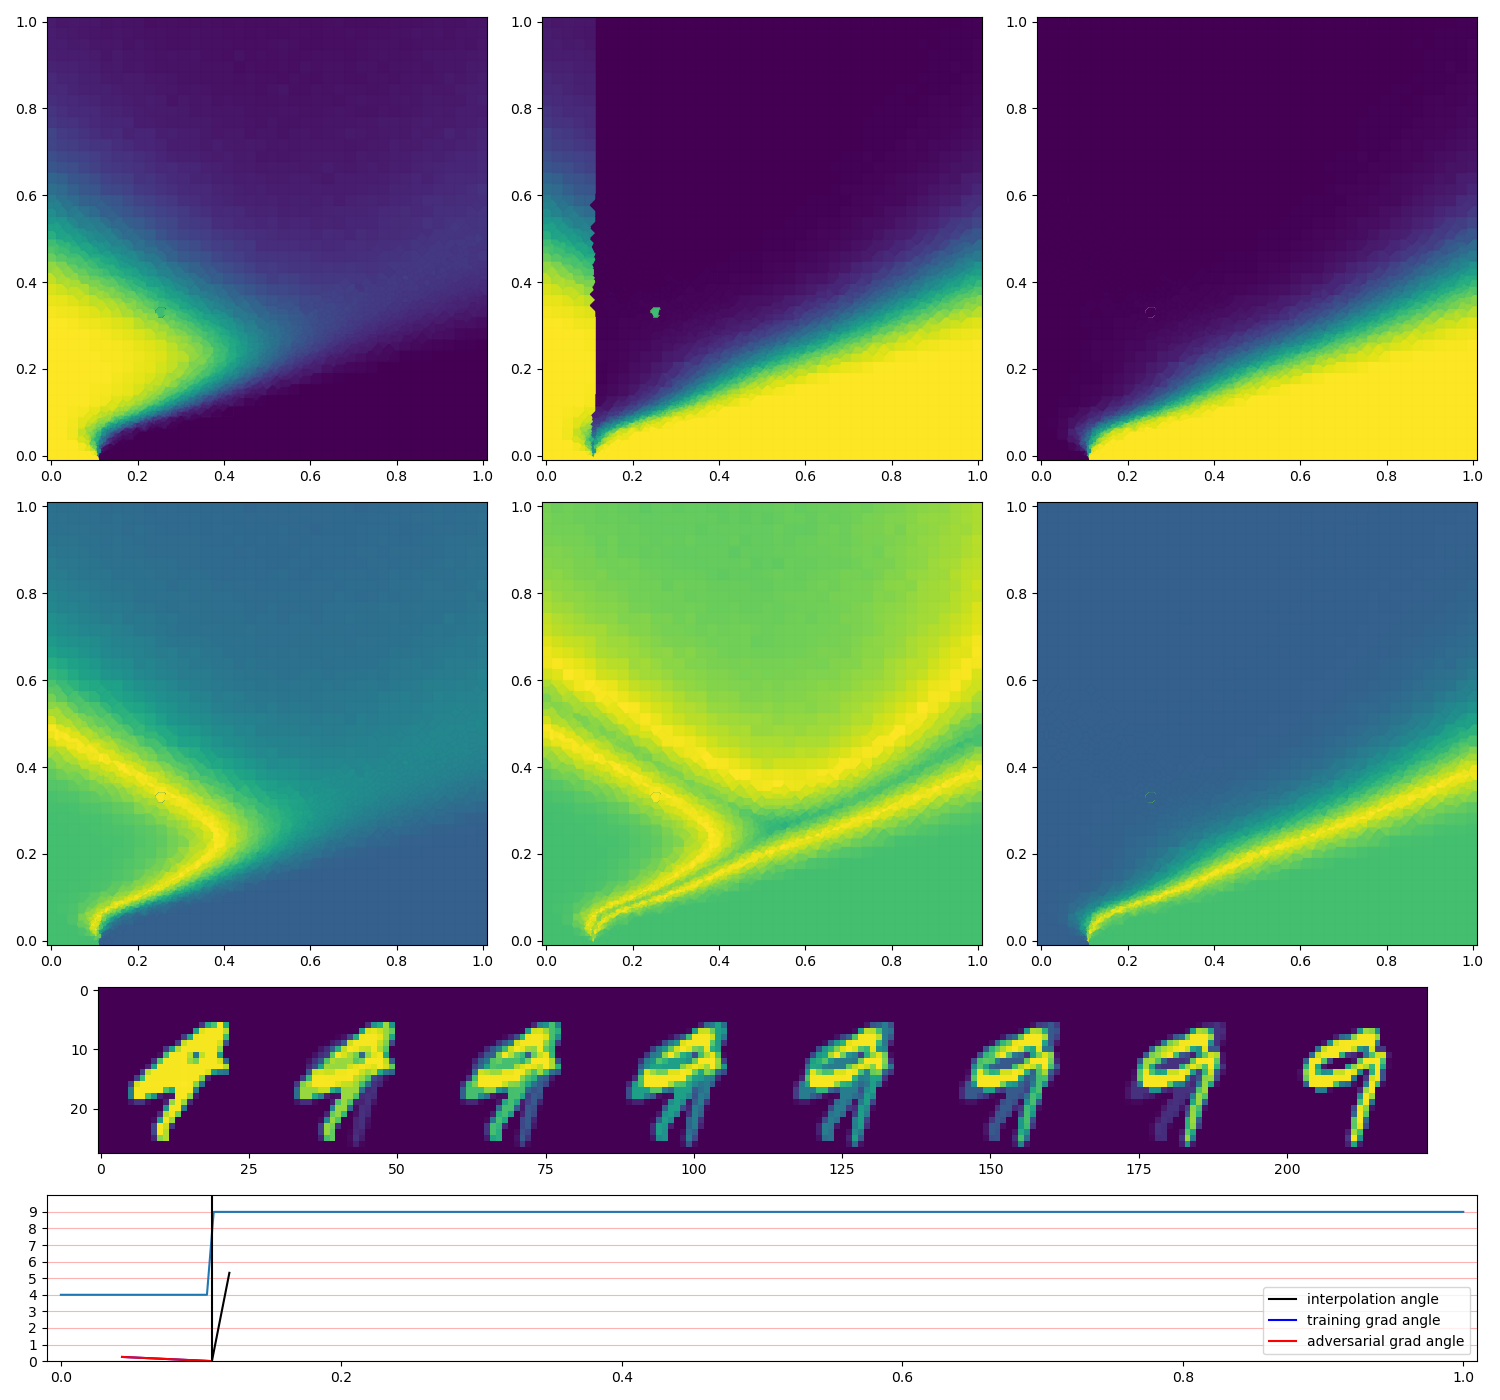
\includegraphics[width=0.42\textwidth]{stab-mnist-C32-50-50-10-0.001-eval-1e-06-none-4-9-db_interp-stability-51.png}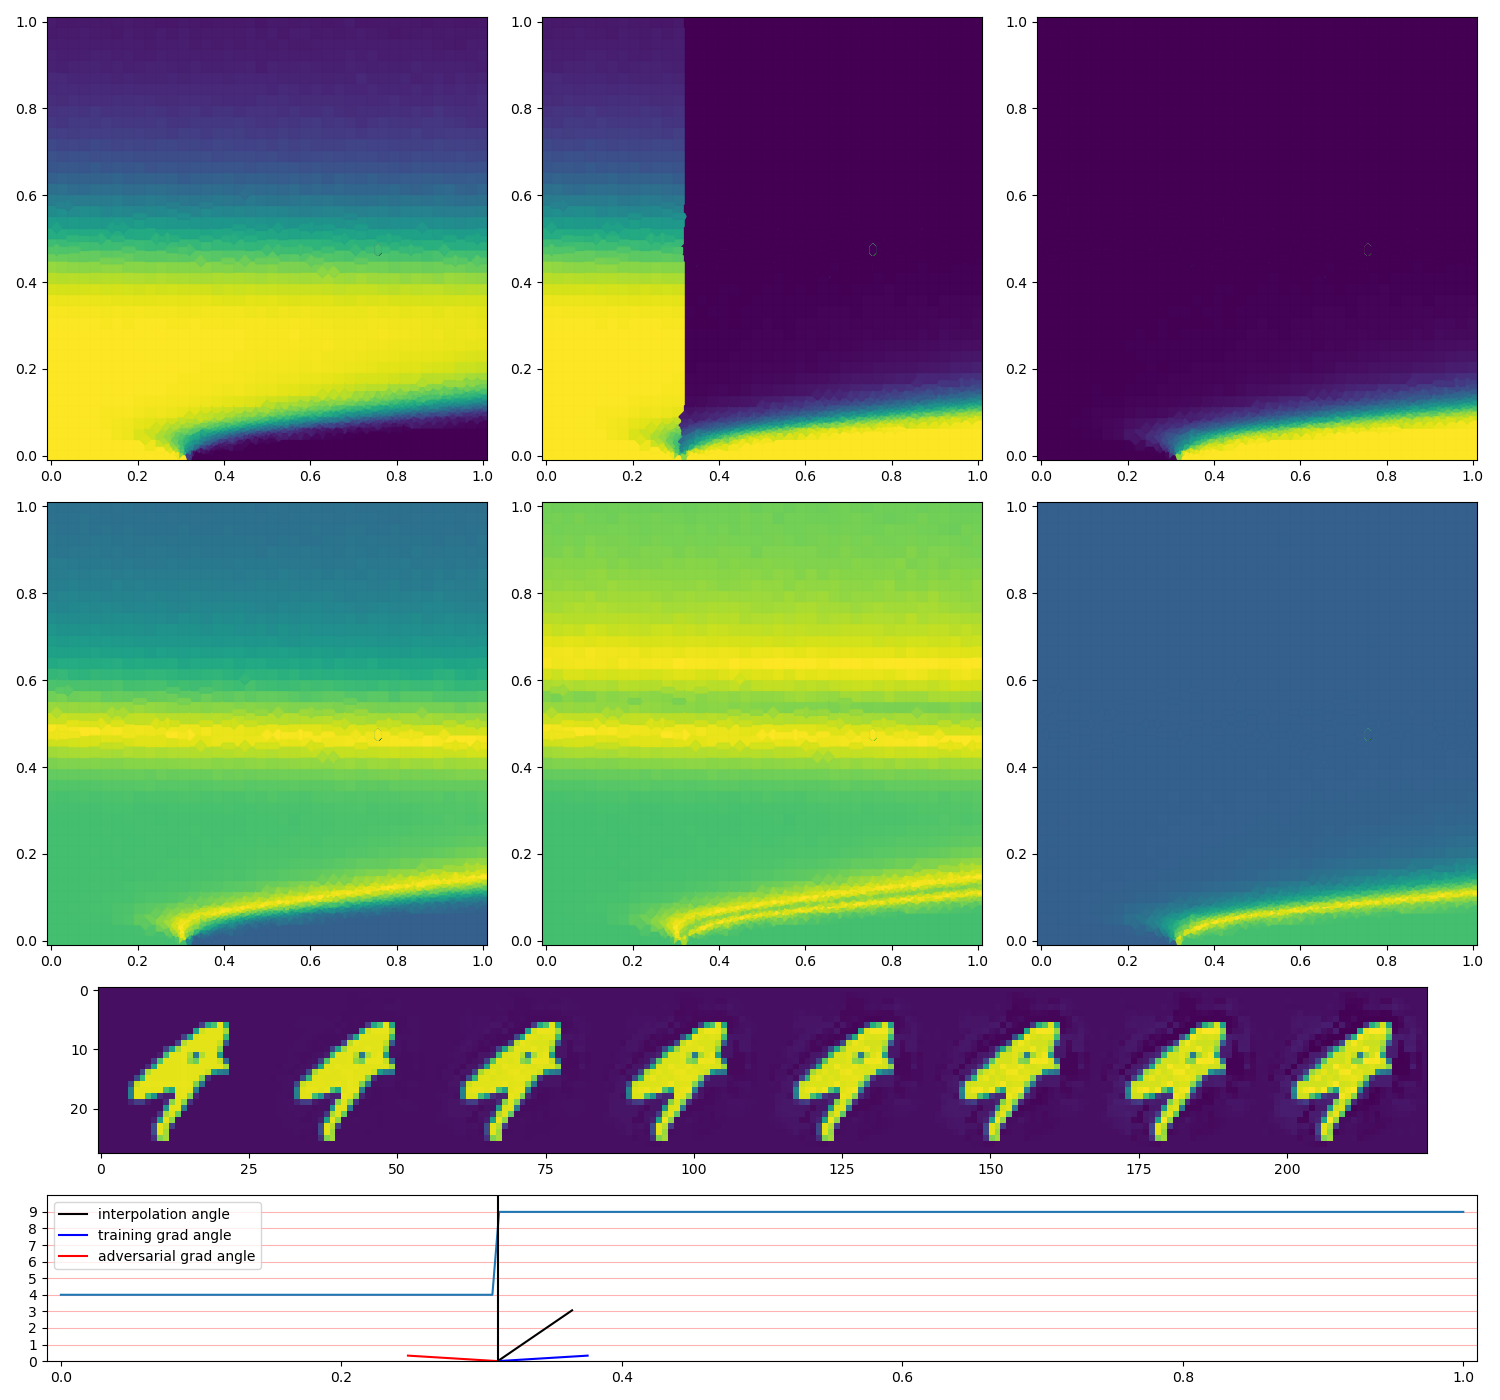
\includegraphics[width=0.42\textwidth]{stab-mnist-C32-50-50-10-0.001-eval-1e-06-pgd-4-9-db_interp-stability-51.png} 
  
  \usebeamerfont{author}\usebeamercolor[fg]{black}\insertauthor\par
  \usebeamerfont{institute}\insertinstitute\par
  \usebeamerfont{date}\normalsize\insertdate\par
  \usebeamercolor[fg]{titlegraphic}\inserttitlegraphic
}


\begin{document}

\begin{frame}
  \titlepage
\centering

\end{frame}

% Introduction
% historical timeline
% reference some explanatory pictures
% introduce some notation
% main takeaways the mathematical elements are simple but notation is
%a limitation.
% Introduction
% historical timeline
% reference some explanatory pictures
% introduce some notation
% main takeaways the mathematical elements are simple but notation is
%a limitation.
\part{Introduction} % Main chapter title
\label{Chapter1} % For referencing the chapter elsewhere, use \ref{Chapter1} 

% \begin{frame}[fragile]
% \frametitle{Neural Network}

% \scalebox{.9}{
% \begin{frame}[fragile]
% \frametitle{Neural Network}

% \scalebox{.9}{
% }
% \end{frame}

%%%%%%%%%%%%%%%%%%%%%%%%%%%%%%%%%%%%%%%%%(1)
\begin{frame}
  \frametitle{Goals}
  \begin{itemize}
      % \item<1-> Describe brief history of machine-learning. 
      \item<1-> Understand (mathematically) what Artificial Neural
        Networks (ANNs) are and how they are being used. 
      \item<2-> Define a geometric approach to interpreting neural
        network classifiers. 
      \item<3-> Connect geometric approach with concept of 
        robustness. 
      \item<4-> Define a kernel based representation which allows application
        of kernel based tools to ANNs
      \item<5-> Leverage our kernel based representation and these
        tools to get some useful results!
      \item<6-> Lay out further work which will connect representation
        approach to the geometric properties observed earlier. 
  \end{itemize}
\end{frame}

% transition from task specific models to foundation models --
% Models are starting to have a "general" geometric understanding of
% the data. 
\section{Background}

\begin{frame}
  \frametitle{History : Beginnings in Theory of Cognition}
  \begin{itemize}
     \item<1->  The mechanics of cognition are described in the context of
      computation by ~\citet{mcculloch1943logical}. 
      \item<2-> The perceptron $f(x) = A(w \cdot x + b)$, the
        most granular element of a neural network, is proposed by
        ~\citet{rosenblatt1958perceptron}. 
      \item<3->  Perceptrons are assembled into multilevel (deep)
        networks ($A_n \circ f_n \circ
        \cdots \circ f_3 \circ A_2 \circ f_2 \circ
        A_1 \cdots f_1$) by ~\citet{ivakhnenko1965cybernetic}
      \item<5->  ~\citet{minsky1969perceptrons} present a proof that
        basic perceptrons could not encode exclusive-or. 
      \item<6->  Neural Networks become disassociated from Cognitive
        Science and Computational Limitations curtail industrial
        applications. 
      \item<7-> Interest in Neural Networks wanes. 
  \end{itemize}
\end{frame}

\begin{frame}
  \frametitle{History : Revolution}
  \begin{itemize}
      \item<1-> ~\citet{linnainmaa1970representation} proposes
        a computation for gradients of large-scale multi-parameter
 models in his masters thesis. Back-Propagation is born!
      \item<2->  A Harvard student,  ~\citep{werbos1974beyond},
        applies this technique to ANNs. 
      \item<3->  ~\citet{mcclelland1986parallel} propose distributed
        processing in the context of cognition allowing tree-like
        computations to be processed in separate computing threads. 
      \item<4-> Finally, these pieces are brought together by
        ~\citet{lecun1989backpropagation}. 
      \item<5->  ~\citep{lecun1995convolutional} invent convolutional
        neural networks which are more capable and scale more
        cheaply.
        \item <6-> This completed tools is applied to the
        lucrative task of handwriting recognition
        ~\citep{lecun1998gradient} and the commercial viability of
        ANNs is established. 

  \end{itemize}
\end{frame}

\begin{frame}
  \frametitle{History : Explosion}
  \begin{itemize}
     \item<1-> Neural Networks' industrial success fuels a new wave of
       serious research and development including the now famous
       PyTorch ~\citep{Collobert2002TorchAM} 
       
     \item<2-> Geoffrey Hinton is among the first to comprehensively understand
       how to scale ``deep'' learning models
       ~\citep{hinton2006reducing, hinton2006fast} along with Samy
       Bengio ~\citep{bengio2009learning}. 

       % \item<3-> Recurrent networks, applying  earlier work on
       %   Long-Short-Term-Memory (LSTM) networks
       %   ~\citep{hochreiter1997long} to overcome vanishing gradients, are implemented
       %   ~\citep{mikolov2010recurrent}. 

       \item<3-> Recurrent ANNs are applied to natural
language processing ~\citep{collobert2011natural}
       \item<4-> ~\citet{szegedy2013} discover easily scalable
         adversarial attacks against neural networks!

      \item<5-> Networks trained on Google's ImageNet database (>14M
        images, >20K categories) outperform humans on classification
        tasks \citep{SCHMIDHUBER201585}
      \visible<4>{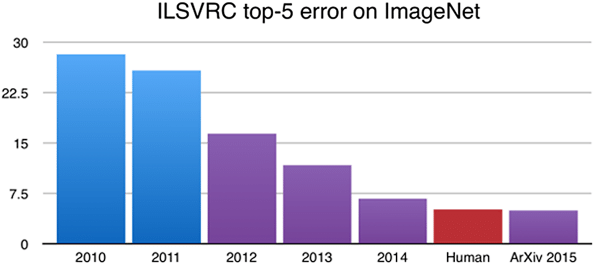
\includegraphics[width=7cm]{imnet_progress.png}}
  \end{itemize}
\end{frame}


\subsection{Structure}
% In this subsection we give a mathematical description of artificial neural networks. 

% %TODO: change this definition to something very vague and general -- use wikipedia 
% \begin{definition}{A \textbf{Neuron} is  }
%    a nonlinear operator that takes input in $\R^n$ to $\R$, historically designed to emulate the activation characteristics of an organic neuron.
%    \end{definition}

% \begin{frame}
%   \frametitle{Definitions : ANN}
% \begin{definition}{A \textbf{Neuron} is  } a nonlinear operator that
%   takes input in $\R^n$ to $\R$, historically designed to emulate the
%   activation characteristics of an organic neuron. A collection of
%   neurons that are connected via a (usually directed) graph structure
%   are known as an \emph{Artificial Neural Network (ANN)}.
% \end{definition}


% \end{frame}
\begin{frame}
  \frametitle{Definitions : Building Blocks}

The fundamental building blocks of most ANNs are artificial neurons which we will refer to as \emph{perceptrons}.

\begin{definition}{A \textbf{Perceptron} is  }
\label{perceptron}
a function $P_{\vec w}: \R^n \to \R$ which has \emph{weights} $\vec
w \in \R^n$ corresponding with each element of an input vector $\vec
x\in \R^n$ and a bias $b \in \R$:
\[P_{\vec w}(\vec x) = f(\left(\ip{\vec w,\vec x} + b\right)\]
\[P_{\vec w}(\vec x) = f\left(b + \sum_{i = 1}^n w_i x_i\right)\]
where $f: \R \to \R$ is continuous. The function $f$ is called the \textbf{activation function} for $P$. 
\end{definition}

\end{frame}

\begin{frame}
  \frametitle{Definitions : Perceptron}
  Perceptrons have a few notable properties
  \begin{itemize}
  \item $w \cdot x + b$ is linear.
    \item The activation function $f$ must contain all non-linearity
      needed for universal function approximation.
      \item In order to approximate arbitrary nonlinear functions, $f$ must
        not be linear ~\citep{attali1997approximations}.
        \item Arbitrarily many perceptrons can be connected in a
          tree-structure.
\end{itemize}
\end{frame}
      

\begin{frame}
 \frametitle{Definitions : ReLU}
\begin{definition}{The Rectified Linear Unit (ReLU) function is}
\label{relu}
   \[\relu(x) = \begin{cases} 0, & x \leq 0;\\
       x, & x > 0,\end{cases}\]
 \end{definition}

\begin{itemize}
    \item ~\citet{glorot2011deep} showed that
      Rectified Linear Units (ReLU) can out-perform smoother
      activation functions e.g. sigmoids.
    \item ReLU Networks even converge faster according to
      ~\citet{nair_rectified_nodate}!
    \item  ~\citet{petersen2018optimal} demonstrated that this single
      nonlinearity of this activation function
at $x = 0$ is sufficient to guarantee existence of $\epsilon$ approximation of smooth functions
\end{itemize}
\end{frame}





% In general ANNs 
% must not be cyclic and, for convenience, are often arranged into
% independent layers. An early roadblock for neural networks was a proof
% by ~\citet{minsky1969perceptrons} that single layers of perceptrons
% could not encode exclusive-or. ~\citet{kak1993training} demonstrated
% that depth, the number of layers in a neural network, is a key factor in its ability to approximate complicated functions including exclusive-or . For this reason, modern ANNs are usually composed of many layers (3-100). The most common instance of a neural network model is a fully connected \emph{feed forward (FF)} configuration. In this configuration data enters as an input layer which is fed into each of the nodes in the first layer of neurons. Output of the first layer is fed into each of the nodes in the second layer, and so on until the output of the final layer is fed into an output filter which generates the final result of the neural network. 



\begin{frame}
  \frametitle{Example : Fully Connected Feed Forward Network}
% In this example of a FF network, an input vector in $\R^7$ is mapped to a
% an output in $\R^3$ which is fed into a classifier. Each blue circle
% represents a perceptron with the ReLU activation function. 
\centering
\scalebox{.9}{
\begin{tikzpicture}[shorten >=1pt,->,draw=black!50, node distance=\layersep]
    \tikzstyle{every pin edge}=[<-,shorten <=1pt]
    \tikzstyle{neuron}=[circle,fill=black!25,minimum size=9pt,inner sep=0pt]
    \tikzstyle{input neuron}=[neuron, fill=green!50];
    \tikzstyle{output neuron}=[neuron, fill=red!50];
    \tikzstyle{hidden neuron}=[neuron, fill=blue!50];
    \tikzstyle{annot} = [text width=4em, text centered]

    % Draw the input layer nodes
    \foreach \name / \y in {1,...,7}
    % This is the same as writing \foreach \name / \y in {1/1,2/2,3/3,4/4}
        \node[input neuron] (I-\name) at (0,-\y) {};
%pin=left:Input \#\y
    % Draw the hidden layer nodes
    \foreach \name / \y in {1,...,6}
        \path[yshift=-0.5cm]
            node[hidden neuron] (H-\name) at (\layersep,-\y cm) {};

    \foreach \name / \y in {1,...,4}
        \path[yshift=-1.5cm,xshift=2.0cm]
            node[hidden neuron] (HH-\name) at (\layersep,-\y cm) {};

    \foreach \name / \y in {1,...,3}
        \path[yshift=-2cm,xshift=4.0cm]
            node[output neuron] (O-\name) at (\layersep,-\y cm) {};

    % Draw the output layer node
%   \foreach \name / \y in {1,...,3}
%        \path[yshift=-1.5cm,xshift=4.0cm]
%            \node[output neuron] (O-\name) at (\layersep,-\y cm) {};


    % Connect every node in the input layer with every node in the
    % hidden layer.
    \foreach \source in {1,...,7}
        \foreach \dest in {1,...,6}
            \path (I-\source) edge (H-\dest);

    \foreach \source in {1,...,6}
        \foreach \dest in {1,...,4}
            \path (H-\source) edge (HH-\dest);

    % Connect every node in the hidden layer with the output layer
    \foreach \source in {1,...,4}
        \foreach \dest in {1,...,3}
            \path (HH-\source) edge (O-\dest);

    % Annotate the layers
  \node [rectangle, draw, minimum height=6.2cm, text width=.8cm, text
  centered, left =.8cm of I-4] (mm) {Data};

    \foreach \source in {1,...,7}
        \path [line] (mm.east|-I-\source) -- (I-\source);

    \node[annot,above of=H-1, node distance=2cm] (hl) {Layer 1};
    \node[annot,left of=hl] {Input };
    \node[annot,right of=hl] (h3) {Layer 2} ;
    \node[annot,right of=h3] {Output Layer};
  \node [rectangle, draw, minimum height=5cm, text width=1.6cm, text
  centered, right =6.8cm of I-4] (mc) {Classifier};
    \foreach \source in {1,...,3}
        \path [line] (O-\source) -- (mc.west|-O-\source);


\end{tikzpicture}
}
\end{frame}


% The output of this ANN is fed into a classifier. To complete this
% example, we can define the most common classifier, Softmax:

\begin{frame}
  \frametitle{Definition : Softmax Classifier}
\begin{definition}{Softmax (or the normalized exponential) is the function given by}
\[s : \R^n \to [0,1]^n\]
\[s_j(\vec x) = \frac{e^{x_j}}{\sum_{k = 1}^n e^{x_k}}\]
\end{definition}

\begin{definition}{We can define a classifier which picks the class corresponding with the largest output element from Softmax: }
\[\text{(Output Classification)  }   c_s(\vec x) = \text{argmax}_{i} s_i(\vec{x})\]
\end{definition}
\end{frame}

% % It is important that the classifier admit a directed error function
% During training, the output $y \in \R^n$ from a network can thus be
% compressed using softmax into $[0,1]^n$ as a surrogate for probability
% for each possible class or directly into the classes which we can
% represent as the simplex for the vertices of $[0,1]^n$
% \citep{Bishop:2006:PRM:1162264}. 

% \subsubsection{Convolutional Neural Networks (CNNs)}\label{cnn}

\begin{frame}
  \frametitle{Example : Other Network Structures}
  \begin{itemize}
    \item \textbf{Convolutional Neural Networks} (CNNs) arrange nodes
      spatially and convolve kernels across this spatially producing
      output with multiple channels (corresponding with each
      individual kernel used) and preserving spatial adjacency.
    \item \textbf{Recurrent Neural Networks} (RNNs) admit prior
      network activations as inputs during computation allowing 
      limited ``memory'' while working on time-varying data.
\end{itemize}
\end{frame}
      

\begin{frame}
  \frametitle{Training ANNs}
  \begin{enumerate}
  \item Pick a Training Set
  \item Pick a loss function
     One commonly used loss function for classification is known as Cross-Entropy Loss:
 \begin{definition}{The Cross-Entropy Loss comparing two possible outputs is}
 $L(y,\hat y) = -\sum_i y_i \log \hat y_i$.
 \end{definition}
(Other commonly used loss functions include $L^1$ loss (also referred
to as Mean Absolute Error (MAE)), $L^2$ loss (often referred to as
Mean-Squared-Error (MSE)), and Hinge Loss (also known as SVM loss). )
\item Pick a first-order optimization scheme (ODE solver).
  \end{enumerate}
\end{frame}



\begin{frame}
  \frametitle{Training : Optimization}
  
 To set up the optimization, the loss for each training example must be aggregated. Generally, ANN training is conducted via Empirical Risk Minimization where Empirical Risk is defined for a given loss function $L$ as follows:
 \begin{definition}{Given a loss function $L$, the Empirical Risk over a training dataset $(X,Y)$ of size $N$ is }
 \[R_{\text{emp}}(P_{\vec w}(x) = \dfrac{1}{N} \sum_{(x,y) \in (X,Y)} L(P_{\vec w}(x)), y).\]
 \end{definition}
 We seek parameters $\vec w$ which will minimize $R_{\text{emp}}(P_{w}(x))$. This will be done with gradient-based optimization. 
\end{frame}

\begin{frame}
\frametitle{Computation of Gradient via Backpropagation}

\scalebox{.9}{
\begin{tikzpicture}[shorten >=1pt,->,draw=black!50, node distance=\layersep]

\node[circle, minimum size=19pt, fill=black!25, inner sep=0pt] (n11) at (0,2) {$a^1_1$};
\node[circle, minimum size=19pt, fill=black!25, inner sep=0pt] (n12) at (0,0) {$a^1_2$};
\node[circle, minimum size=19pt, fill=black!25, inner sep=0pt] (n21) at (4,2) {$a^2_1$};
\node[circle, minimum size=19pt, fill=black!25, inner sep=0pt] (n22) at (4,0) {$a^2_2$};
\node[circle, minimum size=19pt, fill=black!25, inner sep=0pt] (n31) at (8,2) {$a^3_1$};
\node[circle, minimum size=19pt, fill=black!25, inner sep=0pt] (n32) at (8,0) {$a^3_2$};

\node (av1) at (0,2.9) {$\Bar{a}^1$};
\node (av2) at (4,2.9) {$\Bar{a}^2$};
\node (av3) at (8,2.9) {$\Bar{a}^3$};

\node (ai1) at (0,3.9) {Index: $i$};
\node (ai2) at (4,3.9) {Index: $\alpha$};
\node (ai3) at (8,3.9) {Index: $\lambda$};

\node (w2) at (2.6,2.9) {$W^2$};
\node (w3) at (6.6,2.9) {$W^3$};


\draw[- triangle 45] (n11)  -- node[rotate=0,shift={(0.3,0.3)}] {$w^2_{1,1}$} (n21);
\draw[- triangle 45] (n11)  -- node[rotate=0,shift={(0.6,0.65)}] {$w^2_{1,2}$} (n22);
\draw[- triangle 45] (n12)  -- node[rotate=0,shift={(0.3,-0.65)}] {$w^2_{2,1}$} (n21);
\draw[- triangle 45] (n12)  -- node[rotate=0,shift={(0.6,-0.3)}] {$w^2_{2,2}$} (n22);

\draw[- triangle 45] (n21)  -- node[rotate=0,shift={(0.3,0.3)}]  {$w^3_{1,1}$} (n31);
\draw[- triangle 45] (n21)  -- node[rotate=0,shift={(0.6,0.65)}] {$w^3_{1,2}$} (n32);
\draw[- triangle 45] (n22)  -- node[rotate=0,shift={(0.3,-0.65)}]  {$w^3_{2,1}$} (n31);
\draw[- triangle 45] (n22)  -- node[rotate=0,shift={(0.6,-0.3)}]  {$w^3_{2,2}$} (n32);
\end{tikzpicture}
}
Where $x^{\text{[layer]}}_{\text{[node in layer], [node in previous
    layer]}}$

Recursively, we will define
\begin{equation}
    a^n_\lambda = A^n(\sum_\alpha w^n_{\alpha, \lambda} a^{n-1}_\alpha)
\end{equation}
\end{frame}

\begin{frame}
  \frametitle{Computation of Gradient via Backpropagation}
Given a loss function $L = \sum_{i} \ell_i(a^n_i)$ where each $\ell_i$ is a loss function on the $i^{\text{th}}$ element of the output, we wish to compute the derivatives $\dfrac{\partial L}{\partial_{w^l_{i,j}}}$ for every $l, i,$ and $j$ which compose the gradient $\nabla L$. Using the diagram above, we can compute this directly for each weight using chain rule:
\begin{align*}
    \dfrac{\partial L}{\partial w^3_{\lambda,\alpha}} &= \dfrac{\partial L}{\partial a^3_{\lambda}} \dfrac{\partial a^3_{\lambda}}{\partial w^3_{\lambda,\alpha}} = \sum_{\lambda=1}^n \ell'_\lambda( a^3_\lambda) A'^3 (\sum_{\alpha=1}^n w^3_{\alpha, \lambda} a_\alpha^2) a^2_\alpha\\    
    %\dfrac{\partial L}{\partial w^2_{\alpha,i} } &= \sum_{\lambda} \dfrac{\partial L}{\partial a^3_{\lambda}} \dfrac{\partial a^3_{\lambda} }{\partial w^3_{\lambda,\alpha}} \dfrac{\partial a^2_\alpha }{ w^2_{\alpha,i}}\\
\end{align*}
Many of the terms of this gradient (e.g. the activations $a^n_i$ and the sums $\sum_{i} w^n_{i,j} a_i$) are computed during forward propagation when using the network to generate output. 

\end{frame}

\begin{frame}
  \frametitle{Computation of Gradient via Backpropagation}
We can see that all of the partials will be of the form 
$\dfrac{\partial L}{\partial w^l_{n, i}} = \delta^l_n a^l_i$ where
$\delta^l_n$  will contain terms which are either pre-computed or can
be computed analytically. We will write this recursively in matrix form: 
% \[
% \delta^l_n = A'^l (a^l_{n}) \sum_{i = 1}^n w^{l+1}_{i, n} \delta^{l+1}_i
% \]
% In matrix form, we have
\[\bar \delta^l = \bar A'^l(W^l \bar a^l) \odot ((W^{l+1})^T \bar \delta^{l+1}\]
Where $\odot$ signifies element-wise multiplication. 

Then we can write the gradient with respect to each layer's matrix $W^l$: 
\[\nabla_{W^l} L = \bar \delta^l \bar a^{(l-1)T}\]
Since this recursion for layer $n$ only requires information from layer $n+1$, this allows us to propagate the error signals that we compute backwards through the network. 

\end{frame}

\begin{frame}{Optimizing Weights}
\begin{definition}{Stochastic Gradient Descent (SGD)}

Given an ANN $N: \R^n \to C$, an initial set of weights for this network $\vec w_0$ (usually a small random perturbation from 0), a set of training data $X$ with labels $Y$, and a learning rate $\eta$, the algorithm is as follows: 

\begin{algorithm}[H]
\caption*{Batch Stochastic Gradient Descent}\label{sgd}
\begin{algorithmic}[H]
\State $w = w_0$
\While{$E(\hat Y, P_w(X))$ (cumulative loss) is still improving} \Comment{ (the stopping condition may require that the weight change by less than $\e$ for some number of iterations or could be a fixed number of steps)}
\State Randomly shuffle $(X,Y)$
\State Draw a small batch $(\hat X, \hat Y) \subset (X, Y)$
\State $w \leftarrow w - \eta \left(\sum_{(x,y) \in (\hat X, \hat Y)}  \nabla L(P_w(\hat x), \hat y)\right)$
\EndWhile
\end{algorithmic}
\end{algorithm}
\end{definition}
\end{frame}

  
% Adversarial Attacks
% introduce attacks
% picture attacks
% get some intuition on transferrence and adversarial robustness
% main takeaways all (most networks) have these vulnerabilities)
%      and adversraial examples are hard to define (separate
%adversarial from perplexing (other term?))
% Chapter Template
\section{Adversarial Attacks}

\label{Chapter2} % Change X to a consecutive number; for referencing this chapter 

%\section{Adversarial Attacks}

\begin{frame}
  \frametitle{Intriguing Properties of Neural Networks \cite{Szegedy2013}}
\begin{figure}[H]
    \centering
\includegraphics[width=5.5cm]{szegedy/negative1.png}\includegraphics[width=5.5cm]{szegedy/negative2.png}
    \caption{Natural Images are in columns 1 and 4, Adversarial images are in columns 3 and 6, and the difference between them (magnified by a factor of 10) is in columns 2 and 5. All images in columns 3 and 6 are classified by AlexNet as "Ostrich" \cite{Szegedy2013}}
    \label{fig:my_label}
\end{figure}
\end{frame}



%%%%%%%%%%%%%%%%%%%%%%%%%%%%%%%%%%%%%%%%%%%(2)
% 2. define classifier
\begin{frame}
\frametitle{Attacks : L-BFGS}
Let $f : \R^m \to \{1,...,k\}$ be a classifier and assume $f$ has an associated continuous loss function denoted by loss$_f : \R^m \times \{1,...,k\} \to \R^+$ and $l$ a target adversarial . \\
\textbf{ Minimize} $\Norm{r}_2$ subject to:
\begin{enumerate}[1.]
\item $f(x + r) = l$
\item $x + r \in [0,1]^m$
\end{enumerate}

The solution is approximated with L-BFGS as implemented in Pytorch or Keras. This technique yields examples that are close to their original counterparts in the $L^2$ sense.
\end{frame}
\begin{frame}{Attacks : L-BFGS : MNIST}
    \begin{figure}[H]
\label{lbfgsa}
\includegraphics[trim=200 185 100 200, clip, width=6cm]{2019-04-10-adverse/mnist_examples/FC200-200-10-2448-O8-A0-attack_summary.png}\includegraphics[trim=200 185 100 200, clip,width=6cm]{2019-04-10-adverse/mnist_examples/FC200-200-10-2448-O8-A1-attack_summary.png}
\includegraphics[trim=200 185 100 200, clip,width=6cm]{2019-04-10-adverse/mnist_examples/FC200-200-10-2448-O8-A2-attack_summary.png}\includegraphics[trim=200 185 100 200, clip,width=6cm]{2019-04-10-adverse/mnist_examples/FC200-200-10-2448-O8-A3-attack_summary.png}
\includegraphics[trim=200 185 100 200, clip,width=6cm]{2019-04-10-adverse/mnist_examples/FC200-200-10-2448-O8-A4-attack_summary.png}\includegraphics[trim=200 185 100 200, clip,width=6cm]{2019-04-10-adverse/mnist_examples/FC200-200-10-2448-O8-A5-attack_summary.png}
\caption{Original images on the left, Perturbation is in the middle, Adversarial Image (total of Original with Perturbation) is on the right. Column 1 shows an original 8 being perturbed to adversarial classes 0, 2, and 4. Column 2 shows adversarial classes 1, 3, and 5}
\end{figure}
\end{frame}
\begin{frame}{Attacks : Distortion}
    Borrowing a metric from Szegedy et al to compare the magnitude of these distortions, we will define
\begin{definition}{Distortion is the $L^2$ norm of the difference between an original image and a perturbed image, divided by the square root of the number of pixels in the image: }
\[\sqrt{\dfrac{\sum_i \hat (x_i - x_i)^2}{n}}\]
\end{definition}
Distortion is $L^2$ magnitude normalized by the square-root of the number of dimensions so that values can be compared for modeling problems with differing numbers of dimensions. 
\end{frame}

\begin{frame}{Attacks : L-BFGS : MNIST}
    \begin{figure}[H]
\label{lbfgsh}
\includegraphics[trim=200 80 100 100, clip, width=12cm]{2019-04-10-adverse/mnist_examples/FC200-200-10-distortion_hist.png}
\caption{A histogram of the distortion measured for each of 900 adversarial examples generated using L-BFGS against the FC-200-200-10 network on Mnist. Mean distortion is 0.089.}
\end{figure}
\end{frame}
%%%%%%%%%%%%%%%%%%%%%%%%%%%%%%%%%%%%%%%%%%%%%%%%%%%%%%%(3)

\begin{frame}{Attacks : L-BFGS : ImageNet}
 \begin{figure}[H]
\label{lbfgsis}
\includegraphics[trim=200 185 100 200, clip, width=6cm]{2019-04-10-adverse/imnet_examples/vgg16-ILSVRC2012_val_00039098-O722-A965-attack_summary.png}\includegraphics[trim=200 185 100 200, clip, width=6cm]{2019-04-10-adverse/imnet_examples/vgg16-ILSVRC2012_val_00027142-O52-A347-attack_summary.png}
\includegraphics[trim=200 185 100 200, clip, width=6cm]{2019-04-10-adverse/imnet_examples/vgg16-ILSVRC2012_val_00029901-O425-A468-attack_summary.png}\includegraphics[trim=200 185 100 200, clip, width=6cm]{2019-04-10-adverse/imnet_examples/ILSVRC2012_val_00001375-Otensor([42])-A694-attack_summary.png}
% \includegraphics[width=7cm]{2019-04-10-adverse/imnet_examples/vgg16-ILSVRC2012_val_00035978-O803-A353-attack_summary.png}
% \includegraphics[width=7cm]{2019-04-10-adverse/imnet_examples/ILSVRC2012_val_00000886-Otensor([940])-A684-attack_summary.png}
\caption{Original images on the left, Perturbation (magnified by a factor of 100) by is in the middle, Adversarial Image (total of Original with Perturbation) is on the right. Adversarial classes are Burrito, Bison, Taxi, and Paddle Wheel (Top Left, Top Right, Bottom Left, Bottom Right)}
\end{figure}   
\end{frame}

\begin{frame}{Attacks : L-BFGS : ImageNet}
    \begin{figure}[H]
\label{lbfgsi}
\includegraphics[trim=200 80 100 100, clip,width=12cm]{2019-04-10-adverse/imnet_examples/distortion_hist.png}
\caption{A histogram of the distortion measured for each of 112 adversarial examples generated using L-BFGS against the VGG16 network on ImageNet images with mean distortion 0.0107}
\end{figure}
\end{frame}

% 3. discuss solving neural networks, i.e. tuning weights. (gradient and
%    back propagation passes error through the network)
% 4. discus doing this computationally with torch or other
%    multi-threading tools
%%%%%%%%%%%%%%%%%%%%%%%%%%%%%%%%%%%%%%%%%%%%%%%%%%%%%%%%%%%%%%(2)
\begin{frame}
\frametitle{Attacks : FGSM}
A single step attack process using the gradient of the loss function $L$ with respect to an image to find the adversarial perturbation \cite{goodfellow_explaining_2014}. for given $\e$, the modified image $\hat x$ is computed as
\begin{equation}
\hat{x} = x + \epsilon \text{sign} (\nabla L (P_w(x),x))
\end{equation}

This method is simpler and much faster to compute than the L-BFGS technique described above, but produces adversarial examples less reliably and with generally larger distortion.

\end{frame}

\begin{frame}
\frametitle{Attacks : IGSM}
In \cite{kurakin_adversarial_2016}
  an iterative application of FGSM was proposed. After each
  iteration, the image is clipped to a $\e L_\infty$ neighborhood of the original. Let $x'_0 = x$, then after $m$ iterations, the adversarial image obtained is:
\begin{equation}
x_{m+1}' = \text{Clip}_{x,\epsilon} \Bigl\{x_m' + \alpha \times \text{sign}(\nabla \ell (F(x'_m),x'_m))  \Bigr\} 
\label{igsm}
\end{equation}
This method is faster than L-BFGS and more reliable than FGSM but still produces examples with greater distortion than L-BFGS. 
\end{frame}

\begin{frame}{Attacks : IGSM : ImageNet}
    \begin{figure}[H]
  \centering
\includegraphics[trim=200 780 1200 212, clip,width=4cm]{2019-04-10-adverse/ILSVRC2012_val_00002900summary_plot.png}\includegraphics[trim=900 780 500 212, clip,width=4cm]{2019-04-10-adverse/ILSVRC2012_val_00002900summary_plot.png}
%\includegraphics[width=12cm]{2019-04-10-adverse/ILSVRC2012_val_00048234summary_plot.png}
\caption{adversarial example generated against VGG16 (ImageNet) with IGSM. Original Image (Rose Hip) on the left, adversarial image (Baseball) on the right. }
\label{fgsmhip}
\end{figure}
\end{frame}


%\section{Introduction}
%%%%%%%%%%%%%%%%%%%%%%%%%%%%%%%%%%%%%%%%%%%%%%%%%%%%%%%%%%%%%%(2)

% Deep Neural Networks (DNNs) and their variants are core to the success
% of modern machine learning as summarized by ~\citet{prakash2018}. They
% have dominated competitions in image processing, optical character
% recognition, object detection, video classification, natural language
% processing, and many other fields ~\citet{SCHMIDHUBER201585}. Ten years
% ago, along the explosion of applications, an interesting property of
% such networks was observed by ~\citet{szegedy2013}. Their approach was to define a loss function
% relating the output of the ANN for a given initial image to a target adversarial 
% output plus the $L^2$-norm of the input and use backpropagation to
% compute gradients -- not on the weights of the neural network, but on
% just the input layer to the network. The solution to this optimization
% problem, efficiently approximated by a gradient-based optimizer, would
% be a slightly perturbed natural input with a highly perturbed
% output. Their experimental results are striking which we can see in
% Figure.~\ref{fig:szegedy}.  More mysteriously, these examples
% are often transferable -- an attack generated against one
% model may succeed against a totally different model. With the
% incredible expansion of the application of universal function
% approximators in machine-learning, their reliability has come to have
% real-world significance. The ability of an image processing vehicle to
% distinguish speed limit versus stop-signs ~\citep{DBLP:journals/corr/EvtimovEFKLPRS17},
% optimization based models are increasingly relied upon by the defense
% intelligence apparatus ~\citep{hutchins2011intelligence}, search
% engines use ML increasingly to
% determine which sources will receive attention when we ask questions
% and even our personal information security may rely on the robustness
% of machine-learning models against adversarial perturbations. In order
% to wisely use these tools, it is crucial that we carefully understand
% their limitations. It is for this reason that mathematical study and
% formulation of the Adversarial problem is critical. 


% Adversarial examples occur when natural data can be perturbed in small
% ways in order to produce a similar input which receives a
% significantly different model output. ``Small'' in this context may
% refer to small in a particular metric or sometimes is referred to in
% the context of human perception. It is important to note that Adversarial
% examples are not just a peculiarity, but seem to occur for most, if
% not all, DNN  classifiers. For example, ~\citet{inevitable2018} used
% isoperimetric inequalities on high dimensional spheres and hypercubes
% to conclude that there is a reasonably high probability that each
% correctly classified data point has a nearby adversarial
% example. ~\citet{ilyas2019adversarial} argued that optimized models use
% some subtle features for classification which are neither intuitive to
% humans nor robust to perturbation. In particular, that ML models can
% efficiently extract features from training data, but that they do not
% connect these features robustly across scales. The prevalence of these
% features is illustrated by ~\citet{madry2018towards} with the simple experiment of adding vast
% quantities of adversarially perturbed data during training
% . Although this method increases
% adversarial robustness at a cost to prediction accuracy ~\citep{tsipras2018robustness}, it does not
% do so very significantly, and leaves behind vulnerabilities that can
% still be reduced to non-robust features ~\citep{inevitable2018}. 

% %There are now a wide variety of attacks which produce adversarial examples and defenses which try to detect them. \todo{[DG]: not sure this is necessary. [K]: This paragraph is incomplete. Do you think there shouldn't be such a paragraph at all? [DG]: Not sure it is needed. If so, it maybe should probably come right at the beginning before the shafahi/are adversarial examples inevitable.}

% For this work, we will take a geometric approach to analyzing 
% robustness, both in terms of the models' understanding of underlying
% data geometry and by carefully defining the decision boundary of a
% model and studying its properties. In this vein, there have been many
% attempts to identify adversarial examples using properties of the
% decision boundary.  ~\citet{Fawzi2018empirical} found that decision
% boundaries tend to have highly curved regions, and these regions tend
% to favor negative curvature, indicating that regions that define
% classes are highly nonconvex. These were found for a variety of DNNs
% and classification  tasks. 
% %They also suggest exploiting this curvature discrepancy to identify when a data point is a natural image and when it is adversarial. 
% A related idea is that adversarial examples often arise within cones, outside of which images are classified in the original class, as observed by ~\citet{roth19aodds}. Many theoretical models of adversarial examples, for instance the dimple model developed by ~\citet{shamir2021}, have high curvature and/or sharp corners as an essential piece of why adversarial examples can exists very close to natural examples.


% \begin{figure}[H]
%     \centering
% \includegraphics[width=7.3cm]{c1_figures/negative1.png}\includegraphics[width=7.3cm]{c1_figures/negative2.png}
%     \caption{Natural Images are in columns 1 and 4, Adversarial images are in columns 3 and 6, and the difference between them (magnified by a factor of 10) is in columns 2 and 5. All images in columns 3 and 6 are classified by AlexNet as "Ostrich" ~\citep{szegedy2013}.}
%     \label{fig:szegedy}
% \end{figure}

% \section{Common Datasets}

% The first step in all machine-learning and in our endeavor to
% understand adversarial attacks is to understand the data on which
% neural networks are built. We will limit our investigation mostly to
% classic image classification problems, although several of our results
% will hold more generally. The Dataset used above in
% Figure.~\ref{fig:szegedy} is known as ImageNet -- a large set of
% labeled images varying in size originally compiled for the ImageNet
% Large Scale Visual Recognition Challenge (ILSVRC ~\citet{ILSVRC15}). This
% dataset and its many subsets has become a standard for image
% classification and feature identification experiments. In the
% experiments that follow, ImageNet will be featured alongside the
% Modified National Institute of Standards and Technology dataset (MNIST ~\citet{MNIST}) which is a database of hand written digits often used to develop image processing and character recognition systems. This dataset is much lower resolution than ImageNet and is therefore experiments run much more quickly on it and require less complex input/output.  

% \section{Common Attack Techniques}
% % TODO : Add massive carlini toolkit reference
% Adversarial attacks are generally produced by introducing an objective
% function which balances the adversarial objective, e.g. \emph{cross-entropy
% loss} defined by ~\citet{good1963maximum} of the source image as a positive
% value to be minimized or with a specific target combined with a
% regularization term in image space (e.g. the $L^2$ norm) which
% penalizes the generated adversary for being too far from its starting
% point. This loss function is combined with an optimization algorithm
% in order to produce an attack. 


% \subsection{L-BFGS minimizing distortion}\label{lbfgs}

% The original attack used by ~\citet{szegedy2013} took advantage of the
% tools they had on  hand for training neural networks to set up a
% box-constrained optimization problem whose approximated solution
% generates these targeted mis-classifications. We will write this
% precisely according to their formulation: \\

% Let $f : \R^m \to \{1,...,k\}$ be a classifier and assume $f$ has an associated continuous loss function denoted by loss$_f : \R^m \times \{1,...,k\} \to \R^+$ and $l$ a target adversarial . \\
% \textbf{ Minimize} $\Norm{r}_2$ subject to:
% \begin{enumerate}[1.]
% \item $f(x + r) = l$
% \item $x + r \in [0,1]^m$
% \end{enumerate}

% The solution is approximated with L-BFGS (see Appendix \ref{appa}) as
% implemented in Pytorch or Keras. This technique yields examples that
% are close to their original counterparts in the $L^2$ sense, but are
% predicted to be another class by the model with high confidence .  \\

% %Find the minimum $c > 0$ for which the minimizer $r$ of the following satisfies $f(x+r) = l$\\

% %minimize $c|r| + $loss$_f(x+r,l)$ subject to $x + r \in [0,1]^m$.

% \paragraph{L-BFGS: Mnist}
% The following examples are prepared by implementing the above technique via pytorch on images from the Mnist dataset with FC200-200-10, a neural network with 2 hidden layers with 200 nodes each:
% \begin{figure}[H]
% \label{lbfgsa}
% \includegraphics[trim=200 185 100 200, clip, width=7cm]{c1_figures/FC200-200-10-2448-O8-A0-attack_summary.png}\includegraphics[trim=200 185 100 200, clip,width=7cm]{c1_figures/FC200-200-10-2448-O8-A1-attack_summary.png}
% \includegraphics[trim=200 185 100 200, clip,width=7cm]{c1_figures/FC200-200-10-2448-O8-A2-attack_summary.png}\includegraphics[trim=200 185 100 200, clip,width=7cm]{c1_figures/FC200-200-10-2448-O8-A3-attack_summary.png}
% \includegraphics[trim=200 185 100 200, clip,width=7cm]{c1_figures/FC200-200-10-2448-O8-A4-attack_summary.png}\includegraphics[trim=200 185 100 200, clip,width=7cm]{c1_figures/FC200-200-10-2448-O8-A5-attack_summary.png}
% \caption{Original images on the left, Perturbation is in the middle, Adversarial Image (total of Original with Perturbation) is on the right. Column 1 shows an original 8 being perturbed to adversarial classes 0, 2, and 4. Column 2 shows adversarial classes 1, 3, and 5}
% \end{figure}
% Borrowing a metric from Szegedy et al to compare the magnitude of these distortions, we will define
% \begin{definition}{Distortion is the $L^2$ norm of the difference between an original image and a perturbed image, divided by the square root of the number of pixels in the image: }
% \[\sqrt{\dfrac{\sum_i \hat (x_i - x_i)^2}{n}}\]
% \end{definition}
% Distortion is $L^2$ magnitude normalized by the square-root of the number of dimensions so that values can be compared for modeling problems with differing numbers of dimensions. 

% The 900 examples generated for the network above had an average distortion of 0.089 with the following distribution of distortions, given in figure 3.

% \begin{figure}[H]
% \label{lbfgsh}
% \includegraphics[trim=200 80 100 100, clip, width=16cm]{c1_figures/FC200-200-10-distortion_hist.png}
% \caption{A histogram of the distortion measured for each of 900 adversarial examples generated using L-BFGS against the FC-200-200-10 network on Mnist. Mean distortion is 0.089.}
% \end{figure}

% \paragraph{L-BFGS: ImageNet}
% \label{lbfgs-s}
% We also tried to replicate the results of ~\citet{szegedy2013} on ImageNet. Attacking VGG16, a well known model from the ILSVRC-2014 competition ~\citep{simonyan2014very}, on ImageNet images with the same technique generates the examples in figure 4: 

% \begin{figure}[H]
% \label{lbfgsis}
% \includegraphics[trim=200 185 100 200, clip, width=8cm]{c1_figures/vgg16-ILSVRC2012_val_00039098-O722-A965-attack_summary.png}\includegraphics[trim=200 185 100 200, clip, width=8cm]{c1_figures/vgg16-ILSVRC2012_val_00027142-O52-A347-attack_summary.png}
% \includegraphics[trim=200 185 100 200, clip, width=8cm]{c1_figures/vgg16-ILSVRC2012_val_00029901-O425-A468-attack_summary.png}\includegraphics[trim=200 185 100 200, clip, width=8cm]{c1_figures/ILSVRC2012_val_00001375-Otensor([42])-A694-attack_summary.png}
% % \includegraphics[width=7cm]{c1_figures/vgg16-ILSVRC2012_val_00035978-O803-A353-attack_summary.png}
% % \includegraphics[width=7cm]{c1_figures/ILSVRC2012_val_00000886-Otensor([940])-A684-attack_summary.png}
% \caption{Original images on the left, Perturbation (magnified by a factor of 100) by is in the middle, Adversarial Image (total of Original with Perturbation) is on the right. }
% \end{figure}

% %The average distortion was 0.01 distributed as seen in figure \ref{lbfgsi}. 

% \begin{figure}[H]
% \label{lbfgsi}
% \includegraphics[trim=200 80 100 100, clip,width=14cm]{c1_figures/distortion_hist.png}
% \caption{A histogram of the distortion measured for each of 112 adversarial examples generated using L-BFGS against the VGG16 network on ImageNet images with mean distortion 0.0107}
% \end{figure}

% \paragraph{Fast Gradient Sign Method (FGSM)} 

% As the study of adversarial examples has expanded, it has become known
% that often very simple single-step attacks are successful and
% sufficiently subtle. ~\citet{goodfellow_explaining_2014} proposed one
% such attack which we have also implemented. This is a single step
% attack process which uses the sign of the gradient of the loss
% function $L$  with respect to the image to find the adversarial
% perturbation . For given $\e$, the modified  image $\hat x$ is
% computed as 
% \begin{equation}
% \hat{x} = x + \epsilon \text{sign} (\nabla L (P_w(x),x))
% \end{equation}

% This method is simpler and much faster to compute than the L-BFGS technique described above, but produces adversarial examples less reliably and with generally larger distortion. Performance was similar but inferior to the Iterative Gradient Sign Method summarized below.  
% %\[\hat x = x + \e \sign(\Delta \ell(F(x'_m),x'_m))\]

% \paragraph{Iterative Gradient Sign Method (IGSM)}
% \label{igsm-s}
% In work by ~\citet{kurakin_adversarial_2016}
%   an iterative application of FGSM was proposed. After each
%   iteration, the image is clipped to a $\e L_\infty$ neighborhood of the original. Let $x'_0 = x$, then after $m$ iterations, the adversarial image obtained is:
% \begin{equation}
% x_{m+1}' = \text{Clip}_{x,\epsilon} \Bigl\{x_m' + \alpha \times \text{sign}(\nabla \ell (F(x'_m),x'_m))  \Bigr\} 
% \label{igsm}
% \end{equation}
% This method is faster than L-BFGS and more reliable than FGSM but still produces examples with greater distortion than L-BFGS. 
% %  \[x'_{m + 1} = \text{Clip}_{x,\e} \{ x'_m + \alpha \times
% %  \sign(\Delta \ell(F(x'_m),x'_m))\] 
% \begin{figure}[H]
%   \centering
% \includegraphics[trim=200 110 1200 102, clip,width=4cm]{c1_figures/ILSVRC2012_val_00002900summary_plot.png}\includegraphics[trim=900 110 500 102, clip,width=4cm]{c1_figures/ILSVRC2012_val_00002900summary_plot.png}
% %\includegraphics[width=12cm]{c1_figures/ILSVRC2012_val_00048234summary_plot.png}
% \label{fgsmhip}
% \caption{adversarial example generated against VGG16 (ImageNet) with IGSM. Original Image on the left, adversarial image and added noise (ratio of variance adversarial noise/original image: 0.0000999) on the right. }
% \end{figure}

% %The attacks contained in figure ~\ref{fgsmhip} were generated with IGSM against VGG16


% \subsection{Other Attacks}
% The following attack techniques are also prevalent in the literature 

% \paragraph{Jacobian-based Saliency Map Attack (JSMA)} Another attack noted by  ~\citet{papernot_limitations_2015}
%   estimates the \emph{saliency map}, a rating for each of the input features (e.g. each pixel) on how influential it is for causing the model to predict a particular class with respect to the model output ~\citep{wiyatno2018saliency}. This attack modifies the pixels that are most salient. This is a targeted attack, and saliency is designed to find the pixel which increases the classifier's output for the target class while tending to decrease the output for other classes.

% \paragraph{Deep Fool (DFool)} A technique proposed by ~\citet{moosavi-dezfooli_deepfool:_2015}
%   to generate an un-targeted iterative attack. 
% This method approximates the classifier as a linear decision boundary and then finds the smallest perturbation needed to cross that boundary.
% This attack minimizes $L_2$ norm with respect to  to the original image.

% \paragraph{Carlini \& Wagner (C\&W)} In work by ~\citet{carlini_towards_2016}
%   an adversarial attack is proposed which updates the loss function such that it jointly minimizes $L_p$ and a custom differentiable loss function based on un-normalized outputs of the classifier (\textit{logits}). 
% Let $Z_k$ denote the logits of a model for a given class $k$, and $\kappa$ a margin parameter. Then C\&W tries to minimize:
% \begin{equation}
% || x - \hat{x} ||_p + c* max\left(Z_k(\hat{x}_y) - max\{Z_k(\hat{x}) : k \neq y\},-\kappa\right)
% \end{equation}

% \subsection{Attack Standards and Toolbox}

% Since adversarial robustness has expanded as a field, many papers have
% been released pushing various methods for defending against
% adversarial attacks. While initially this approach -- producing a
% defense that fit a narrow context and releasing it to the community
% for evaluation was seen as useful. However, most such approaches would
% inevitably face simple rebuttals by small modification of the attack
% techniques used. Carlini and their group gained a particular
% reputation for brief rebuttals ~\citep{carlini_towards_2016, papernot_cleverhans_2016} of such methods, to the prolific extent
% that it has now become a de facto standard. These approaches were
% finally codified by ~\citet{tramer2020adaptive} in the form of a set of
% guidelines that should be used to attack any proposed defense before
% releasing it to the community. This high bar has greatly reduced the
% number of low quality defenses which gain attention, but it has also
% demonstrated the incredible difficulty of producing successful general
% defenses against adversarial attacks. Ironically despite its poor
% performance, the strategy of adversarial training proposed by
% ~\citet{tramer2019adversarial} is one of the few
% defenses which have maintained any advantage under the Tramer/Carlini
% adaptive framework. 


% \section{Theory of Adversarial Examples}

% Despite the prevalence of studies developing and analyzing adversarial
% attacks, the field is characterized by a plethora of definitions for
% what it means to be ``adversarial''. We will analyze a few of these in
% order to develop our own precise definitions. Indeed, defining an
% adversarial example is intimately related with the task of
% identification, which leaves a paradox of sorts: If we can precisely
% define an adversarial example and that definition allows us to
% identify them, then that definition constitutes a perfect defense. In
% practice, however, we know this is at least not trivial. 
% % summarize:
% % odds are odd
% % features not bugs (and rebuttal?)
% % dimpled manifolds

%\section{Defining ``Adversarial''}

% ~\citet{roth19aodds} proposed a statistical method to identify adversarial examples from natural data. Their main idea was to consider how the last layer in the neural network (the logit layer) would behave on small perturbations of a natural example. %, i.e., on $x+\varepsilon n$ where $x$ is a natural example, $\varepsilon>0$ is small, and $n \sim N(0,I)$.  
% This is then compared to the behavior of a potential adversarial example. If it differs by a predetermined threshold, the example is flagged as adversarial. Successfully flagging adversarial examples in this way works best when adversarial examples tend to perturb toward the original class from which the adversarial example was perturbed. However, this is not always the case.
% It was shown by ~\citet{hosseini2019odds} that it is possible to produce adversarial examples, for instance using a logit mimicry attack, that instead of perturbing an adversarial example toward the true class, actually perturb to some other background class. In fact, we will see in Section \ref{sec:mnist} that the emergence of a background class, which was observed as well by ~\citet{roth19aodds}, is quite common. 

% We primarily consider adversarial examples for classifiers.  To wit, let $X$ be a set of possible data and let $L$ be a set of labels. We will consider classifier as a map $\CC: X \to L$. In general $X$ may be much larger than the actual space from which our data are drawn. If the data actually come from a submanifold of $X$, we call this the \emph{data submanifold}. The data submanifold may not be a strict submanifold, and we often do not know the shape or even dimension of it.

% Data is drawn from a distribution $\mu$ on $X$ that is usually not known. The overarching goal of classification is to produce a classifier such that $\CC$ is as good as possible on the support of $\mu$. 
% We define $X_N \subseteq X$ to be the support of $\mu$ and call it the set of \emph{natural data}. 
% Usually our classification problem is the following: given a set of i.i.d. samples $\Sigma \sim \mu$
% , where we consider $\Sigma \subseteq X_N$, 
% and a classifier $\CC_\Sigma$ on $\Sigma$, find a classifier $\CC$ on $X$ such that $\CC$ lies in some class of ``good functions'' in such a way that it is relatively good at interpolating and/or extrapolating $\CC_\Sigma$. In particular, we hope that $\CC$ is as accurate as possible on the support of $\mu$, which we call the ``natural data.'' % \todo{[K]: To a ML audience, it seems to me a bit overkill to describe the idea of statistical learning. Also, this isn't how they would likely describe it, so it could put people off. DG: Agreed, we can probably eliminate this.}
% The classifier $\CC$ partitions $X$ into classes, each of which is defined as $\CC^{-1}(\ell)$ for some $\ell \in L$. Points on the boundaries of these classes do not have a clear choice of label, and the points in $X$ on the boundaries of the classes make up the \emph{decision boundary} for $\CC$.

% To build up to a mathematical framework for adversarial attacks in the
% context of geometric analysis, we develop definitions and terms to
% refer to adversarial examples without relying on subjective
% characteristics like human vision. Let $X$ denote a set of possible
% data and $L$ denote a set of labels that distinguish the different
% classes. We are now ready to define adversarial examples.We now define
% adversarial examples. 

% \begin{frame}
%   \frametitle{Defining Adversarial Examples : Untargeted}
  
% \begin{definition} \label{def:advers}
% Let $d$ be a metric on $X$, let $x\in X$ have label $\ell\in L$, and let $\CC:X\to L$ be a classifier.  We say that $x$ admits an \emph{$(\e,d)$--adversarial example} to $\CC$ if there exists $\hat x \in X$ such that $d(x,\hat x) < \e$ and $\CC(\hat x) \neq \ell$.
% Consider a point $x \in X$ with corresponding class $\ell \in C$ and a classifier $\CC: X \to C$. We say that $x$ admits an \emph{$(\e,d)-$adversarial example} on $\CC$ if there exists a point $\hat x$ such that $d(x,\hat x) < \e$ and $\CC(\hat x) \neq c$. 
% \end{definition}

% One typically considers Definition \ref{def:advers} in the context of small $\e$. 
% Often consideration is made of when such a misclassification is a result of an intentionally act by an adversary. 
% There are various methods of producing adversarial examples which are
% discussed later.
% \end{frame}
% \begin{frame}
%   \frametitle{Defining Adversarial Examples : Targeted}

% In some cases, the adversarial label is explicitly targeted:
% \begin{definition}
% Let $d$ be a metric on $X$, let $x\in X$ have label $\ell\in L$, and let $\CC:X\to L$ be a classifier.  Let $\varepsilon>0$ and $\ell_t\neq \ell$ be fixed but arbitrary. We say that $x$ admits an \emph{$(\varepsilon,d,\ell_t)$--targeted adversarial example} to $\mathcal{C}$ if there exists $\hat{x}\in X$ such that $d(x,\hat{x})<\varepsilon$ and $\CC(\hat{x})=\ell_t$.
% Consider a point $x \in X$ with corresponding class $\ell \in C$ and a classifier $\CC: X \to C$. We say that $x$ admits an \emph{$(\e,d,\ell_t)-$targeted adversarial example} on $\CC$ if there exists a point $\hat x$ such that $d(x,\hat x) < \e$ and $\CC(\hat x) = \ell_t$. 
% \end{definition}
% \end{frame}
\begin{frame}{Defining Adversarial Examples}
    \begin{definition}
Consider a point $x \in X$ with corresponding class $c \in C$ and a classifier $\CC: X \to C$. We say that $x$ admits an \emph{$(\e,d)-$adversarial example} on $\CC$ if there exists a point $\hat x$ such that $d(x,\hat x) < \e$ and $\CC(\hat x) \neq c$. 
\end{definition}
This definition refers to the most general case of intentional mis-classification. The adversarial class can also be explicitly targeted:
\begin{definition}
Consider a point $x \in X$ with corresponding class $c \in C$ and a classifier $\CC: X \to C$. We say that $x$ admits an \emph{$(\e,d,c_t)-$targeted adversarial example} on $\CC$ if there exists a point $\hat x$ such that $d(x,\hat x) < \e$ and $\CC(\hat x) = c_t$. 
\end{definition}
\end{frame}


% These definitions rely on a metric $d$, emphasizing the reliance on the choice of distance to understand notions of closeness. From here on, we will assume that $(X,d)$ is a Euclidean vector space with $d$ being the Euclidean metric. This will allow for the use of standard Gaussian distributions as well.% \todo{[K]: The part about Gaussians here is unclear. [DG]: What I mean here is that one needs a distance metric to define Gaussian distributions. Maybe it is not relevant here?}


% Note that there is no restriction on whether adversarial examples come from the set of natural examples, and typically we will assume that they do not so that we can draw a contrast. 
% We define adversarial examples, sometimes called adversarial attacks, against classifiers
% to be small perturbations from natural data that significantly change the classifier output. See Definition \ref{def:advers} for a formal definition.
% ~\citet{szegedy2013} realized that the same computational tools
% used to train DNN classifiers could be used to generate attacks that would
% confuse them. Their approach was to define a loss function
% relating the output of the DNN for a given initial image to a target adversarial 
% output plus the $L^2$-norm of the input and use backpropagation to 
% compute gradients -- not on the weights of the neural network, but on
% just the input layer to the network. The solution to this optimization
% problem, efficiently approximated by a gradient-based optimizer, would
% be a slightly perturbed natural input with a highly perturbed
% output. There has since been significant work describing methods of producing and identifying
% adversarial examples. In the next sections, we describe some of the most relevant
% to our work here.

% Their experimental results are striking:\\

% \begin{figure}[t]
%    \centering
% \includegraphics[width=7.3cm]{negative1.png}\includegraphics[width=7.3cm]{negative2.png}
%    \caption{Natural Images are in columns 1 and 4, Adversarial images are in columns 3 and 6, and the difference between them (magnified by a factor of 10) is in columns 2 and 5. All images in columns 3 and 6 are classified by AlexNet as "Ostrich" ~\citep{szegedy2013}}
%    \label{fig:my_label}
% \end{figure}

% The Dataset used above is known as ImageNet -- a large set of labeled images varying in size originally compiled for the ImageNet Large Scale Visual Recognition Challenge (ILSVRC). This dataset and its many subsets has become a standard for image classification and feature identification experiments. In the experiments that follow, ImageNet will be featured alongside the Modified National Institute of Standards and Technology (MNIST) dataset which is a database of hand written digits often used to develop image processing and character recognition systems. This dataset is much lower resolution than ImageNet and is therefore experiments run much more quickly on it and require less complex input/output.  

% %%%%%%%%%%%%%%%%%%%%%%%%%%%%%%%%%%%%%%%%%%%%%%%%%%%%%%%%%%%%%%%%%%%%%%%%%%%%%%%%%%%%%%%%%%%%%%%%%%%%%%%%%%%%%%%%%%%%%%%%%%%%%%%%%%%%%%%%%%%%%%%%%%%%%%%%%%%%%%%%%%%%%%%%%%%%%%%%%%%%%%%%%%%%%%%%%%%%%%%%%%%%%%%%%%%%%%%%%%%%%%%%%%%%%%%%%%%%%%%%%%%%%%%%%%%%%%%%





% Persistence
% carefully pose some definitions for adversarial examples
% develop persistence metric and talk about how it is used
\newcommand{\RR}{I\!\!R} %real numbers
\newcommand{\Nat}{I\!\!N} %natural numbers

% Persistence
% carefully pose some definitions for adversarial examples
% develop persistence metric and talk about how it is used

\section{Persistent Classification}
\label{Chapter3}

% \begin{frame}
%   \frametitle{Chapter Goals}
%   \begin{enumerate}
%     \item Define a spatial metric for classification persistence
%       according to arbitrary neural networks. 
%     \item Apply this metric to adversarial examples to show that many
%       are unstable
%     \item Examine connection among predictive accuracy, attack
%       distortion, and persistence.
%   \item Relate all of these observations to the dimpled manifold
%     hypothesis for adversarial examples. \end{enumerate}
% \end{frame}
        

% Some hypotheses underlying the existence of adversarial examples for classification problems are the high-dimensionality of the data, high codimension in the ambient space of the data manifolds of interest, and/or that the structure of machine learning models may encourage classifiers to develop decision boundaries close to data points. 

% This article proposes a new framework for studying adversarial examples that does not depend directly on the distance to the decision boundary. 
% Similarly to the smoothed classifier literature, we define a (natural or adversarial) data point to be $(\gamma,\sigma)$-stable if the probability of the same classification is at least $\gamma$ for points sampled in a Gaussian neighborhood of the point with a given standard deviation $\sigma$. 
% We focus on studying the differences between persistence metrics along interpolants of natural and adversarial points.
% We show that adversarial examples have significantly lower persistence than natural examples for large neural networks in the context of the MNIST and ImageNet datasets. 
% We connect this lack of persistence with decision boundary geometry by measuring angles of interpolants with respect to decision boundaries.
% Finally, we connect this approach with robustness by developing a manifold alignment gradient metric and demonstrating the increase in robustness that can be achieved when training with the addition of this metric. 

% \section{Introduction}

% Deep Neural Networks (DNNs) and their variants are core to the
% success of modern machine learning ~\citep{prakash2018}, and have
% dominated competitions in image processing, optical character
% recognition, object detection, video classification, natural
% language processing, and many other fields
% \citep{SCHMIDHUBER201585}. Yet such classifiers are notoriously
% susceptible to manipulation via adversarial examples
% ~\citep{szegedy2013}.

\begin{frame}
  \frametitle{Background}

 Adversarial examples are not just a peculiarity, but seem to occur
 for most, if not all, DNN classifiers. For example,
 \citet{inevitable2018} used isoperimetric inequalities on high
 dimensional spheres and hypercubes to conclude that there is a
 reasonably high probability that a correctly classified data point
 has a nearby adversarial example.\\

 This has been reiterated using mixed integer linear programs to rigorously check minimum distances necessary to achieve adversarial conditions ~\citep{tjeng2017evaluating}. \citet{ilyas2019adversarial} showed that adversarial examples can arise from features that are good for classification but not robust to perturbation. 
\end{frame}
  
% There have been many attempts to identify adversarial examples using
% properties of the decision boundary. \citet{Fawzi2018empirical} found
% that decision boundaries tend to have highly curved regions, and these
% regions tend to favor negative curvature, indicating that regions that
% define classes are highly nonconvex. The purpose of this work is to
% investigate these geometric properties related to the decision
% boundaries. We will do this by proposing a notion of stability that is
% more nuanced than simply measuring distance to the decision boundary,
% and is also capable of elucidating information about the curvature of
% the nearby decision boundary.

% \begin{frame}
%   \frametitle{Justification}
%   We will develop a statistic extending
%  prior work on smoothed classifiers by \citet{cohen2019certified}. \\

% We will be checking some geometric properties related to the alignment of gradients
%   with human perception \citep{ganz2022perceptually,
%     kaur2019perceptually, shah2021input} and with the related
%   underlying manifold \citep{kaur2019perceptually,
%     ilyas2019adversarial} which may imply robustness.\\

% \end{frame}

% \begin{frame}
%   \frametitle{Justifications}

%   The main hypothesis we seek to investigate is proposed by
%   ~\citet{shamir2021dimpled} and defines smooth manifold-like
%   structures along which model gradients with respect to input must
%   vary.  For our purposes Manifold Aligned Gradients (MAG) will refer to the property that the gradients of a model with respect to model inputs follow a given data
%   manifold $\mathcal{M}$. \\

%  We believe these geometric properties are related
%  to why smoothing methods have been useful in robustness tasks
%  ~\citep{cohen2019certified, lecuyer2019certified, li2019certified}. We propose three approaches in order to connect robustness with geometric properties of the decision boundary learned by ANNs: 

% \end{frame}

\begin{frame}
  \frametitle{Contributions}
 \begin{enumerate}
     \item We propose and implement two metrics based on the success of smoothed classification techniques:  $(\gamma,\sigma)$-stability and $\gamma$-persistence defined with reference to a classifier and a given point (which can be either a natural or adversarial image, for example) and demonstrate their validity for analyzing adversarial examples. 
     \item We interpolate across decision boundaries using our persistence metric to demonstrate an inconsistency at the crossing of a decision boundary when interpolating from natural to adversarial examples.
     \item We demonstrate via direct interpolation across decision boundaries and measurement of angles of interpolating vectors relative to the decision boundary itself that dimensionality is not solely responsible for geometric vulnerability of neural networks to adversarial attack. 
 \end{enumerate}
 \end{frame}

% \section{Motivation and related work}

% Our work is intended to shed light on the existence and prevalence of adversarial examples to DNN classifiers. It is closely related to other attempts to characterize robustness to adversarial perturbations, and here we give a detailed comparison.

 \begin{frame}
   \frametitle{Related Work : Distance-based robustness}

   \begin{itemize}
     % A typical approach to robustness of a classifier is to consider
\item  \citet{khoury2018} define a classifier to be robust if the class of
 each point in the data manifold is contained in a sufficiently large
 ball that is entirely contained in the same class. Larger minimum
 radius of this cover means more robust. 
\item  Robustness by measuring distances from the data manifold to the decision boundary
 ~\citep{Wang2020Improving, xu2023exploring, he2018decision}.

% The larger the
% balls, the more robust the classifier. It is then shown that if
% training sets are sufficiently dense in relation to the reach of the
% decision axis, the classifier will be robust in the sense that it
% classifies nearby points correctly. In practice, we do not know that
% the data is so well-positioned, and it is quite possible, especially
% in high dimensions,
 \item Radii in practice can be extremely small, as evidenced by
 results on the prevalence of adversarial examples, e.g., work by
 \citet{inevitable2018} and in evaluation of ReLU networks with mixed
 integer linear programming e.g., work by ~\citet{tjeng2017evaluating}.

\item \citet{tsipras2018robustness} investigated robustness in terms of how
  small perturbations affect the the average loss of a
  classifier. They define robust accuracy in terms of how often an
  adversarially perturbed example classifies correctly.

  \item \citet{gilmer2018adversarial} use the expected distance to
 the nearest different class (when drawing a data point from the data
 distribution) to capture robustness
  %They
% define standard accuracy of a classifier in terms of how often it
% classifies correctly, and  It was shown
% that sometimes accuracy of a classifier can result in poor robust
% accuracy. , and then show that an accurate
% classifier can result in a small distance to the nearest different
% class in high dimensions when the data is drawn from concentric
% spheres. May recent works ~\citep{he2018decision, chen2023aware,
%   jin2022roby} have linked robustness with decision boundary dynamics,
% both by augmenting training with data near decision boundaries, or
% with dynamics related to distances from decision boundaries. We
% acknowledge the validity of this work, but will address some of its
% primary limitations by carefully studying the dynamics and orientation
% of the decision boundary relative to model data.
\end{itemize}
\end{frame}
% \begin{frame}
% \frametitle{Related Work : Curvature}
% \begin{itemize}
% \item \citet{roth19aodds} observe that adversarial examples often arise within cones,
%   outside of which images are classified in the original class.

%   \item Many theoretical models of
%  adversarial examples, for instance the dimple model developed by
%  \citet{shamir2021}, have high curvature and/or sharp corners as an
%  essential piece of why adversarial examples can exists very close to
%  natural examples.
%  \item Fixed distance based metrics are overly sensitive to sharp
%    curvature and these cones. \textbf{Hypothesis} : a weaker (less
%    strict) distance based metric may help examine the effective
%    curvature around data.

%  \end{itemize}
% \end{frame}


% \begin{frame}
%   \frametitle {Adversarial detection via sampling}
%   \begin{itemize}
    
% % While adversarial examples often occur, they still may be rare in the
% % sense that most perturbations do not produce adversarial
% % examples.
%     \item \citet{yu2019new} invert the adversarial attack process
%       around a test point to
%       ask how ``easy'' it is to find examples of other classes near
%       that point using gradient descent.
%       \item This method has been generalized with
%  the developing of smoothed classification methods
%  ~\citep{cohen2019certified, lecuyer2019certified, li2019certified}
%  which at varying stages of evaluation add noise to the effect of
%  smoothing output and identifying adversaries due to their higher
%  sensitifity to perturbation.
%  \item These methods suffer from significant
%  computational complexity ~\citep{kumar2020curse} and have been shown
%  to have fundamental limitations in their ability to rigorously certify
%  robustness ~\citep{blum2020random, yang2020randomized}.

%  %We will generalize this approach into a metric which will allow us to
%  %directly study these limitations in order to better understand how
%  %geometric properties have given rise to adversarial vulnerabilities.
%  \item In general, the results of \citet{yu2019new} indicate that considering samples of nearby points, which approximate the computation of integrals, is likely to be more successful than methods that consider only distance to the decision boundary.
%  \end{itemize}
% \end{frame}

% \citet{roth19aodds} proposed a statistical method to identify adversarial examples from natural data. Their main idea was to consider how the last layer in the neural network (the logit layer) would behave on small perturbations of a natural example. %, i.e., on $x+\varepsilon n$ where $x$ is a natural example, $\varepsilon>0$ is small, and $n \sim N(0,I)$.  
% This is then compared to the behavior of a potential adversarial example. 

% It was shown by \citet{hosseini2019odds} that it is possible to produce adversarial examples, for instance using a logit mimicry attack, that instead of perturbing an adversarial example toward the true class, actually perturb to some other background class. In fact, we will see in Section \ref{sec:mnist} that the emergence of a background class, which was observed as well by \citet{roth19aodds}, is quite common. Although many recent approaches have taken advantage of these facts ~\citep{taori2020shifts, lu2022randommasking, Osada_2023_WACV, blau2023classifier} in order to measure and increase robustness, we will leverage these sampling properties to develop a metric directly on decision-boundary dynamics and how they relate to the success of smoothing based robustness. 

% {\bf Manifold Aware Robustness}

% The sensitivity of convolutional neural networks to imperceptible changes in input has thrown into question the true generalization of these models.
% ~\citet{jo2017measuring} study the generalization performance of CNNs by transforming natural image statistics.  % surface level irregularities
% Similarly to our MAG approach, they create a new dataset with well-known properties to allow the testing of their hypothesis.
% They show that CNNs focus on high level image statistics rather than human perceptible features.
% This problem is made worse by the fact that many saliency methods fail basic sanity checks \citep{adebayo2018sanity, kindermans2019reliability}.

% Until recently, it was unclear whether robustness and manifold alignment were directly linked, as the only method to achieve manifold alignment was adversarial training.
% Along with the discovery that smoothed classifiers are perceptually
% aligned, comes the hypothesis that robust models in general share this
% property put forward by ~\citet{kaur2019perceptually}.
% This discovery raises the question of whether this relationship is bidirectional.

% ~\citet{khoury2018} study the geometry of natural images, and create a lower bound for the number of data points required to cover the manifold.
% Unfortunately, they demonstrate that this lower bound is so large as to be intractable.
% ~\citet{shamir2021dimpled} propose using the tangent space of a
% generative model as an estimation of this
% manifold. ~\citet{magai2022topology} thoroughly review certain
% topological properties to demonstrate that neural networks
% intrinsically use relatively few dimensions of variation during
% training and evaluation . ~\citet{vardi2022gradient} demonstrate that even models which satisfy strong conditions related to max margin classifiers are implicitly non-robust. PCA and manifold metrics have been recently used to identify adversarial examples ~\citep{aparne2022pca, nguyen-minh-luu-2022-textual}. We will extend this work to study the relationship between robustness and manifold alignment directly by baking alignment directly into networks and comparing them with another approach to robustness. 

% {\bf Summary.}
%  In Sections \ref{sec:meth} and \ref{sec:experiments}, we will investigate stability of both natural data and adversarial examples by considering sampling from Gaussian distributions centered at a data point with varying standard deviations. Using the standard deviation as a parameter, we are able to derive a statistic for each point that captures how entrenched it is in its class in a way that is less restrictive than the robustness described by \citet{khoury2018}, takes into account the rareness of adversarial examples described by \citet{yu2019new}, builds on the idea of sampling described by \citet{roth19aodds} and \citet{hosseini2019odds}, and represent curvatures in a sense related to \citet{Fawzi2018empirical}. Furthermore, we will relate these stability studies to direct measurement of interpolation incident angles with decision boundaries in Subsection~\ref{subsec:db} and ~\ref{subsec:dbe} and the effect of reduction of data onto a known lower dimensional manifold in Subsections ~\ref{subsec:ma} and ~\ref{subsec:mae}.  

% \section{Methods} \label{sec:meth} % Stability and Persistence

% In this section we will lay out the theoretical framework for studying stability, persistence, and decision boundary corssing-angles. 

\subsection{Stability and Persistence} \label{subsec:stab}
% In this section we define a notion of stability of classification of a point under a given classification model. In the following, $X$ represents the ambient space the data is drawn from (typically $\RR^n$) even if the data lives on a submanifold of $X$, and $L$ is a set of labels (often $\{1,\dots,\ell\}$).  Note that points $x\in X$ can be natural or adversarial points.%The following definition complements the definition for adversarial examples by providing a criteria for the local stability of the classifier about a point, which could be an actual test point or an adversarial example: 

\begin{frame}
  \frametitle{Stability}
\begin{definition}
Let $\CC:X\to L$ be a classifier, $x \in X$, $\gamma\in(0,1)$, and $\sigma>0$. We say $x$ is \emph{$(\gamma,\sigma)$-stable} with respect to $\CC$ if $\mathbb{P}[\CC(x')=\CC(x)] \geq \gamma$ for $x' \sim \rho = N(x, \sigma^2 I)$; i.e. $x'$ is drawn from a Gaussian with variance $\sigma^2$ and mean $x$.
\end{definition}

 In the common setting when $X=\RR^n$, we have
 \[\mathbb{P}[\CC(x')=\CC(x)] = \int_{\RR^n} \mathbbm{1}_{\CC^{-1}(\CC(x))} (x') d\rho (x') = \rho(\CC^{-1}\CC(x)).\]
 Note here that $\CC^{-1}$ denotes preimage. %In the case of images drawn from $\RR^n$, we can write this integral precisely as
% One could substitute various probability measures $\rho$ above with mean $x$ and variance $\sigma^2$ to obtain different measures of stability corresponding to different ways of sampling the neighborhood of a point.  Another natural choice would be sampling the uniform measure on balls of changing radius. Based on the concentration of measure for both of these families of measures we do not anticipate significant qualitative differences in these two approaches. We propose Gaussian sampling because it is also a product measure, which makes it easier to sample and simplifies some other calculations below.

 For the Gaussian measure, the probability above may be written more concretely as
 \begin{equation}\label{EQN:Gaussian}
 \frac{1}{\left(\sqrt{2\pi}\sigma\right)^{n}} \int_{\RR^n} \mathbbm{1}_{\CC^{-1}(\CC(x))} (x')e^{-\frac{\norm{x - x'}^2}{2\sigma^2}} dx'.
 \end{equation}
\end{frame}
% In this work,
\begin{frame}
  \frametitle{Stability Approximation}
  We will conduct experiments in which we estimate this stability for fixed $(\gamma,\sigma)$ pairs via a Monte Carlo sampling, in which case the integral \eqref{EQN:Gaussian} is approximated by taking $N$ i.i.d. samples $x_k \sim \rho$ and computing
 \[
     \frac{\norm{x_k : \CC(x_k) = \CC(x)}}{N}.
 \]
 Note that this quantity converges to the integral \eqref{EQN:Gaussian} as $N\to\infty$ by the Law of Large Numbers.\\

 The ability to adjust the quantity $\gamma$ is important because it is much weaker than a notion of stability that requires a ball that stays away from the decision boundary as by \citet{khoury2018}. By choosing $\gamma$ closer to $1$, we can require the samples to be more within the same class, and by adjusting $\gamma$ to be smaller we can allow more overlap.

\end{frame}
\begin{frame}
  \frametitle{Persistence}
  
% We also propose a related statistic, \emph{persistence}, by fixing a
% particular $\gamma$ and adjusting $\sigma$.
  For any $x\in X$ not on the decision boundary, for any choice of $0<\gamma<1$ there exists a $\sigma_\gamma$ small enough such that if $\sigma < \sigma_\gamma$ then $x$ is $(\gamma,\sigma)$-stable. We can now take the largest such $\sigma_\gamma$ to define persistence.

 \begin{definition}
     Let $\CC:X\to L$ be a classifier, $x \in X$, and $\gamma\in(0,1)$. Let $\sigma_\gamma^*$ be the maximum $\sigma_\gamma$ such that $x$ is $(\gamma, \sigma)$-stable with respect to $\CC$ for all $\sigma<\sigma_\gamma$. We say that $x$ has \emph{$\gamma$-persistence} $\sigma_\gamma^*$.
 \end{definition}

The $\gamma$-persistence quantity $\sigma_\gamma^*$ measures the
stability of the neighborhood of a given $x$ with respect to the
output classification.
%Small persistence indicates that the classifier is unstable in a small neighborhood of $x$, whereas large persistence indicates stability of the classifier in a small neighborhood of $x$. In the later experiments, we have generally taken $\gamma = 0.7$. This choice is arbitrary and chosen to fit the problems considered here. In our experiments, we did not see significant change in results with small changes in the choice of $\gamma$.
\end{frame}

% In our experiments, we numerically estimate $\gamma$-persistence via a bisection algorithm that we term the Bracketing Algorithm.  Briefly, the algorithm first chooses search space bounds $\sigma_{\min}$ and $\sigma_{\max}$ such that $x$ is  $(\gamma,\sigma_{\min})$-stable but is not $(\gamma,\sigma_{\max})$-stable with respect to $\CC$, and then proceeds to evaluate stability by bisection until an approximation of $\sigma_\gamma^*$ is obtained.

% \subsection{Decision Boundaries} \label{subsec:db}

% In order to examine decision boundaries and their properties, we will carefully define the decision boundary in a variety of equivalent formulations. 

% \begin{frame}
%   \frametitle{The Argmax Function in Multi-Class Problems}

%  A central issue when writing classifiers is mapping from continuous outputs or probabilities to discrete sets of classes. Frequently argmax type functions are used to accomplish this mapping. To discuss decision boundaries, we must precisely define argmax and some of its properties. 

%  In practice, argmax is not strictly a function, but rather a mapping from the set of outputs or activations from another model into the power set of a discrete set of classes:

%  \begin{equation}
%      \text{argmax} : \R^k \to \mathcal{P}(C)
%  \end{equation}

%  % Defined this way,
%  We cannot necessarily consider $\text{argmax}$ to be a function in general as the singleton outputs of argmax overlap in an undefined way with other sets from the power set. However, if we restrict our domain carefully, we can identify certain properties. 
% \end{frame}

\begin{frame}
  \frametitle{Argmax Decision Boundaries }
 \begin{figure}[!ht]
\begin{center}
\begin{tikzpicture}
  \draw[->] (-0.5, 0) -- (3.5, 0) node[right] {$x$};
  \draw[->] (0, -0.5) -- (0, 3.5) node[above] {$y$};
  \node at (1, 2) (c1) {Class 1};
  \node at (2, 1) (c2) {Class 2};
  \draw[-, fill, blue, opacity=.3] (0, 3) -- (3, 3) -- (0, 0);
  \draw[-, fill, red, opacity=.3] (3, 0) -- (3, 3) -- (0, 0);
  \draw[scale=1, domain=0:3, smooth, variable=\x, black, line width=0.45mm] plot ({\x}, {\x});
  %\draw[scale=0.5, domain=-3:3, smooth, variable=\y, red]  plot ({\y*\y}, {\y});
\end{tikzpicture}\begin{tikzpicture}
  \draw[->] (-0.5, 0) -- (3.5, 0) node[right] {$x$};
  \draw[->] (0, -0.5) -- (0, 3.5) node[above] {$y$};
  \node at (1, 2) (c1) {Class 1};
  \node at (2, 1) (c2) {Class 2};
  \draw[-, fill, blue, opacity=.3] (0, 3) -- (3, 3) -- (0, 0);
  \draw[-, fill, red, opacity=.3] (3, 0) -- (3, 3) -- (0, 0);
  \draw[scale=1, domain=0:3, smooth, variable=\x, black, line width=0.45mm] plot ({\x}, {\x});
  \draw[-, orange, line width=0.45mm] (0,3) -- (3, 0);
  %\draw[scale=0.5, domain=-3:3, smooth, variable=\y, red]  plot ({\y*\y}, {\y});
\end{tikzpicture}


 \caption{Decision boundary in $[0,1] \times [0,1]$ (left) and decision boundary restricted to probabilities (right) If the output of $F$ are \emph{probabilities} which add to one, then all points of $x$ will map to the orange line on the right side of Figure~\ref{fig:pdb}. }
 \label{fig:pdb}
 \end{center}
 \end{figure}
\end{frame}
% Restricting to only the pre-image of the singletons, it should be
% clear that argmax is constant.  Indeed, restricted to the pre-image of
% any set in the power-set, argmax is constant and thus
% continuous. This induces the discrete topology whereby the pre-image
% of an individual singleton is open. Observe that for any point whose
% image is a singleton, one element of the domain vector must exceed the 
% others by $\varepsilon > 0$. We shall use the $\ell^1$ metric for
% distance, and thus if we restrict ourselves to a ball of radius
% $\varepsilon$, then all elements inside this ball will have that
% element still larger than the rest and thus map to the same singleton
% under argmax. Since the union of infinitely many open sets is open in
% $\R^k$, the union of all singleton pre-images is an open
% set. Conveniently this also provides proof that the union of all of
% the non-singleton sets in $\mathcal{P}(C)$ is a closed set. We will
% call this closed set the argmax Decision Boundary. We will list two
% equivalent formulations for this boundary.  

\begin{frame}
  \frametitle{Decision Boundary Definitions}
  
\textbf{Complement Definition}
\begin{definition}
 A point $x$ is in the \emph{decision interior} $D_f'$ for a classifier $f: \mathbb{R}^N -> \mathcal{C}$ if there exists $\delta > 0$ such that $\forall \epsilon < \delta$, $|f(B_\epsilon(x))| = 1$. 

 The \emph{decision boundary} of a classifier $f$ is the closure of the complement of the decision interior $\overline{\{x : x \notin D_f'\}}$. 
\end{definition}
 \textbf{Level Set Definition}

 \begin{definition}
   The decision boundary $D$ of a probability valued function $f$ is the pre-image of a union of all level sets of activations $A_c = {c_1, c_2, ..., c_k}$ defined by a constant $c$ such that for some set of indices $L$, we have $c = c_i$ for every $i$ in $L$ and $c > c_j$ for every $j$ not in $L$. The pre-image of each such set are all $x$ such that $f(x) = A_c$ for some $c$. 
 \end{definition}
 \end{frame}


% \section{Experiments} \label{sec:experiments}

% In this section we investigate the stability and persistence behavior of natural and adversarial examples for MNIST \citep{MNIST} and ImageNet \citep{ILSVRC15} using a variety of different classifiers. For each set of image samples generated for a particular dataset, model, and attack protocol, we study $(\gamma,\sigma)$-stability and $\gamma$-persistence of both natural and adversarial images, and also compute persistence along trajectories from natural to adversarial images. In general, we use $\gamma = 0.7$, and note that the observed behavior does not change significantly for small changes in $\gamma$. While most of the adversarial attacks considered here have a clear target class, the measurement of persistence does not require considering a particular candidate class.  Furthermore, we will evaluate decision boundary incidence angles and apply our conclusions to evaluate models trained with manifold aligned gradients. 

% \subsection{MNIST Experiments}

% Since MNIST is relatively small compared to ImageNet, we trained several classifiers with various architectures and complexities and implemented the adversarial attacks directly. Adversarial examples were generated against each of these models using Iterative Gradient Sign Method (IGSM \citep{kurakin_adversarial_2016}) and Limited-memory Broyden-Fletcher-Goldfarb-Shanno (L-BFGS \citep{liu1989limited}).

% \subsubsection{Investigation of $(\gamma, \sigma)$-stability on MNIST}\label{sec:mnist}

\subsection{Experiments}
\begin{frame}
  \frametitle{Experiments : MNIST}
   We begin by sampling gaussians around test points relative to a fully connected ReLU network with layers of size
   784, 100, 20, and 10 and small regularization $\lambda = 10^{-7}$
   which is trained on the standard MNIST training set. \\

   %We then start with a randomly selected MNIST test image $x_1$ from the \texttt{1}'s class and generate adversarial examples $x_0,x_2,\dots,x_9$ using IGSM for each target class other than \texttt{1}. The neighborhoods around each $x_i$ are examined by generating 1000 i.i.d. samples from $N(x_i,\sigma^2I)$ for each of 100 equally spaced standard deviations $\sigma\in(0,1.6)$. Figure \ref{fgsmo} shows the results of the Gaussian perturbations of a natural example $x_1$ of the class labeled \texttt{1} and the results of Gaussian perturbations of the adversarial example $x_0$ targeted at the class labeled \texttt{0}. We provide other examples of $x_2,\ldots,x_9$ in the supplementary materials. Note that the original image is very stable under perturbation, while the adversarial image is not. 

 \begin{figure}[!ht]
   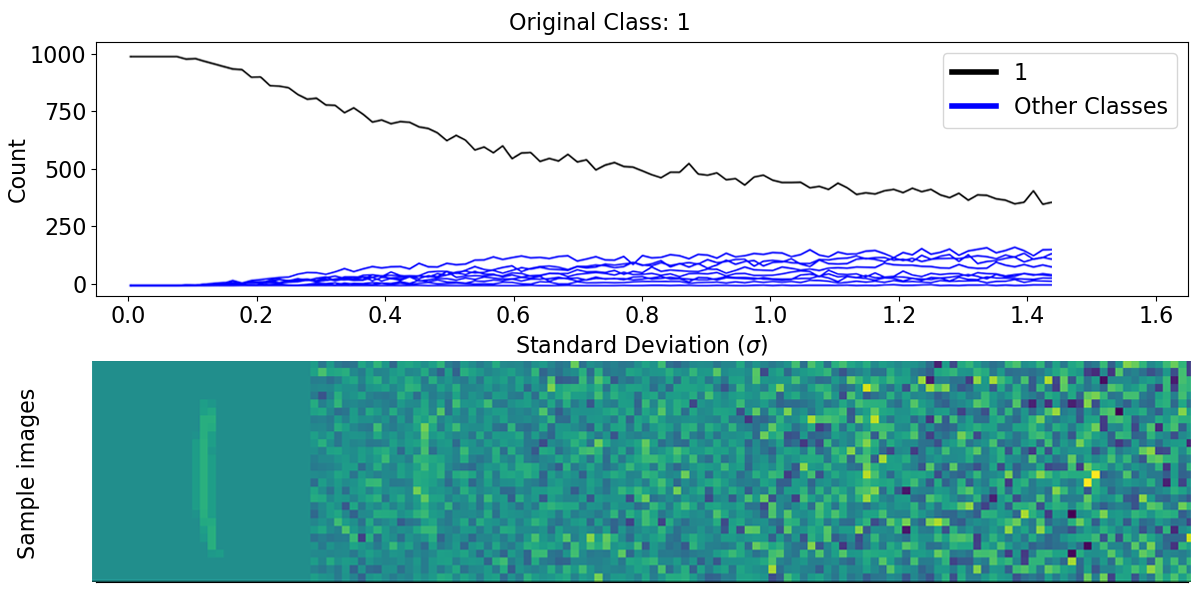
\includegraphics[width = .49\textwidth]{c3_figures/MNIST1.png}
   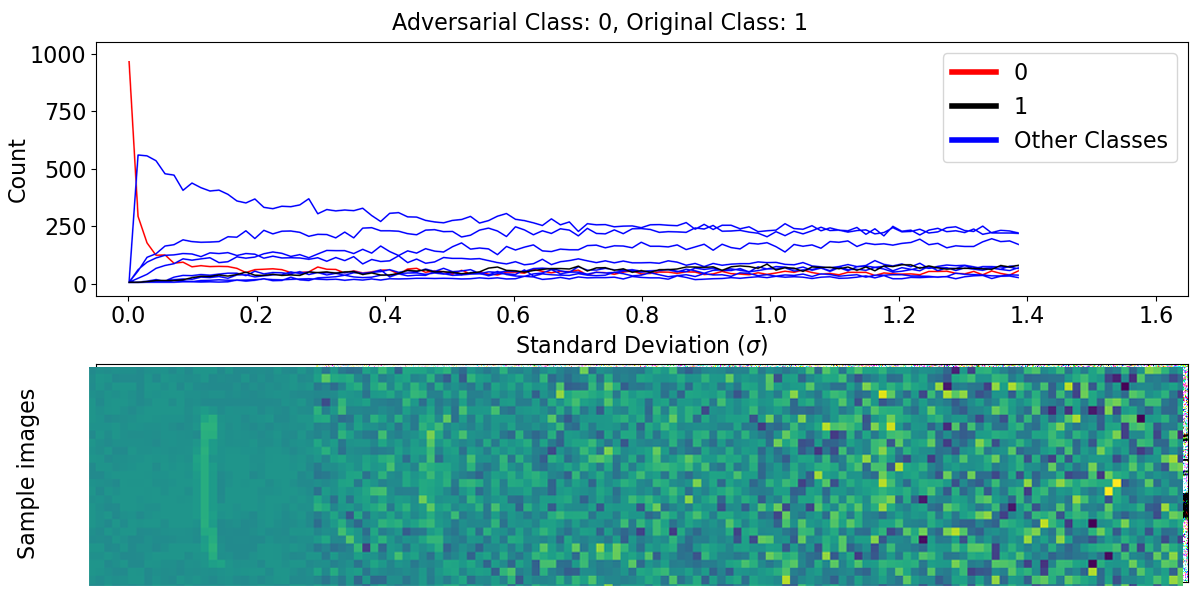
\includegraphics[width = .49\textwidth]{c3_figures/MNIST10.png}
 \caption{Frequency of each class in Gaussian samples with increasing variance around a natural image of class \texttt{1} (left) and around an adversarial attack of that image targeted at \texttt{0} generated using IGSM (right). The adversarial class (\texttt{0}) is shown as a red curve. The natural image class (\texttt{1}) is shown in black. Bottoms show example sample images at different standard deviations for natural (left) and adversarial (right) examples.}\label{fgsmo}
\end{figure}
\end{frame}

% \subsubsection{Persistence of adversarial examples for MNIST}

% To study persistence of adversarial examples on MNIST, we take the same network architecture as in the previous subsection and randomly select 200 MNIST images. For each image, we used IGSM to generate 9 adversarial examples (one for each target class) yielding a total of 1800 adversarial examples. In addition, we randomly sampled 1800 natural MNIST images. For each of the 3600 images, we computed $0.7$-persistence; the results are shown in Figure \ref{fig:IGSMpersistenceMNIST}. One sees that $0.7$-persistence of adversarial examples tends to be significantly smaller than that of natural examples for this classifier, indicating that they are generally less stable than natural images. We will see subsequently that this behavior is typical.

\begin{frame}
  \frametitle{Experiments : MNIST Persistence}
 \begin{figure}[!ht]
 \centering
 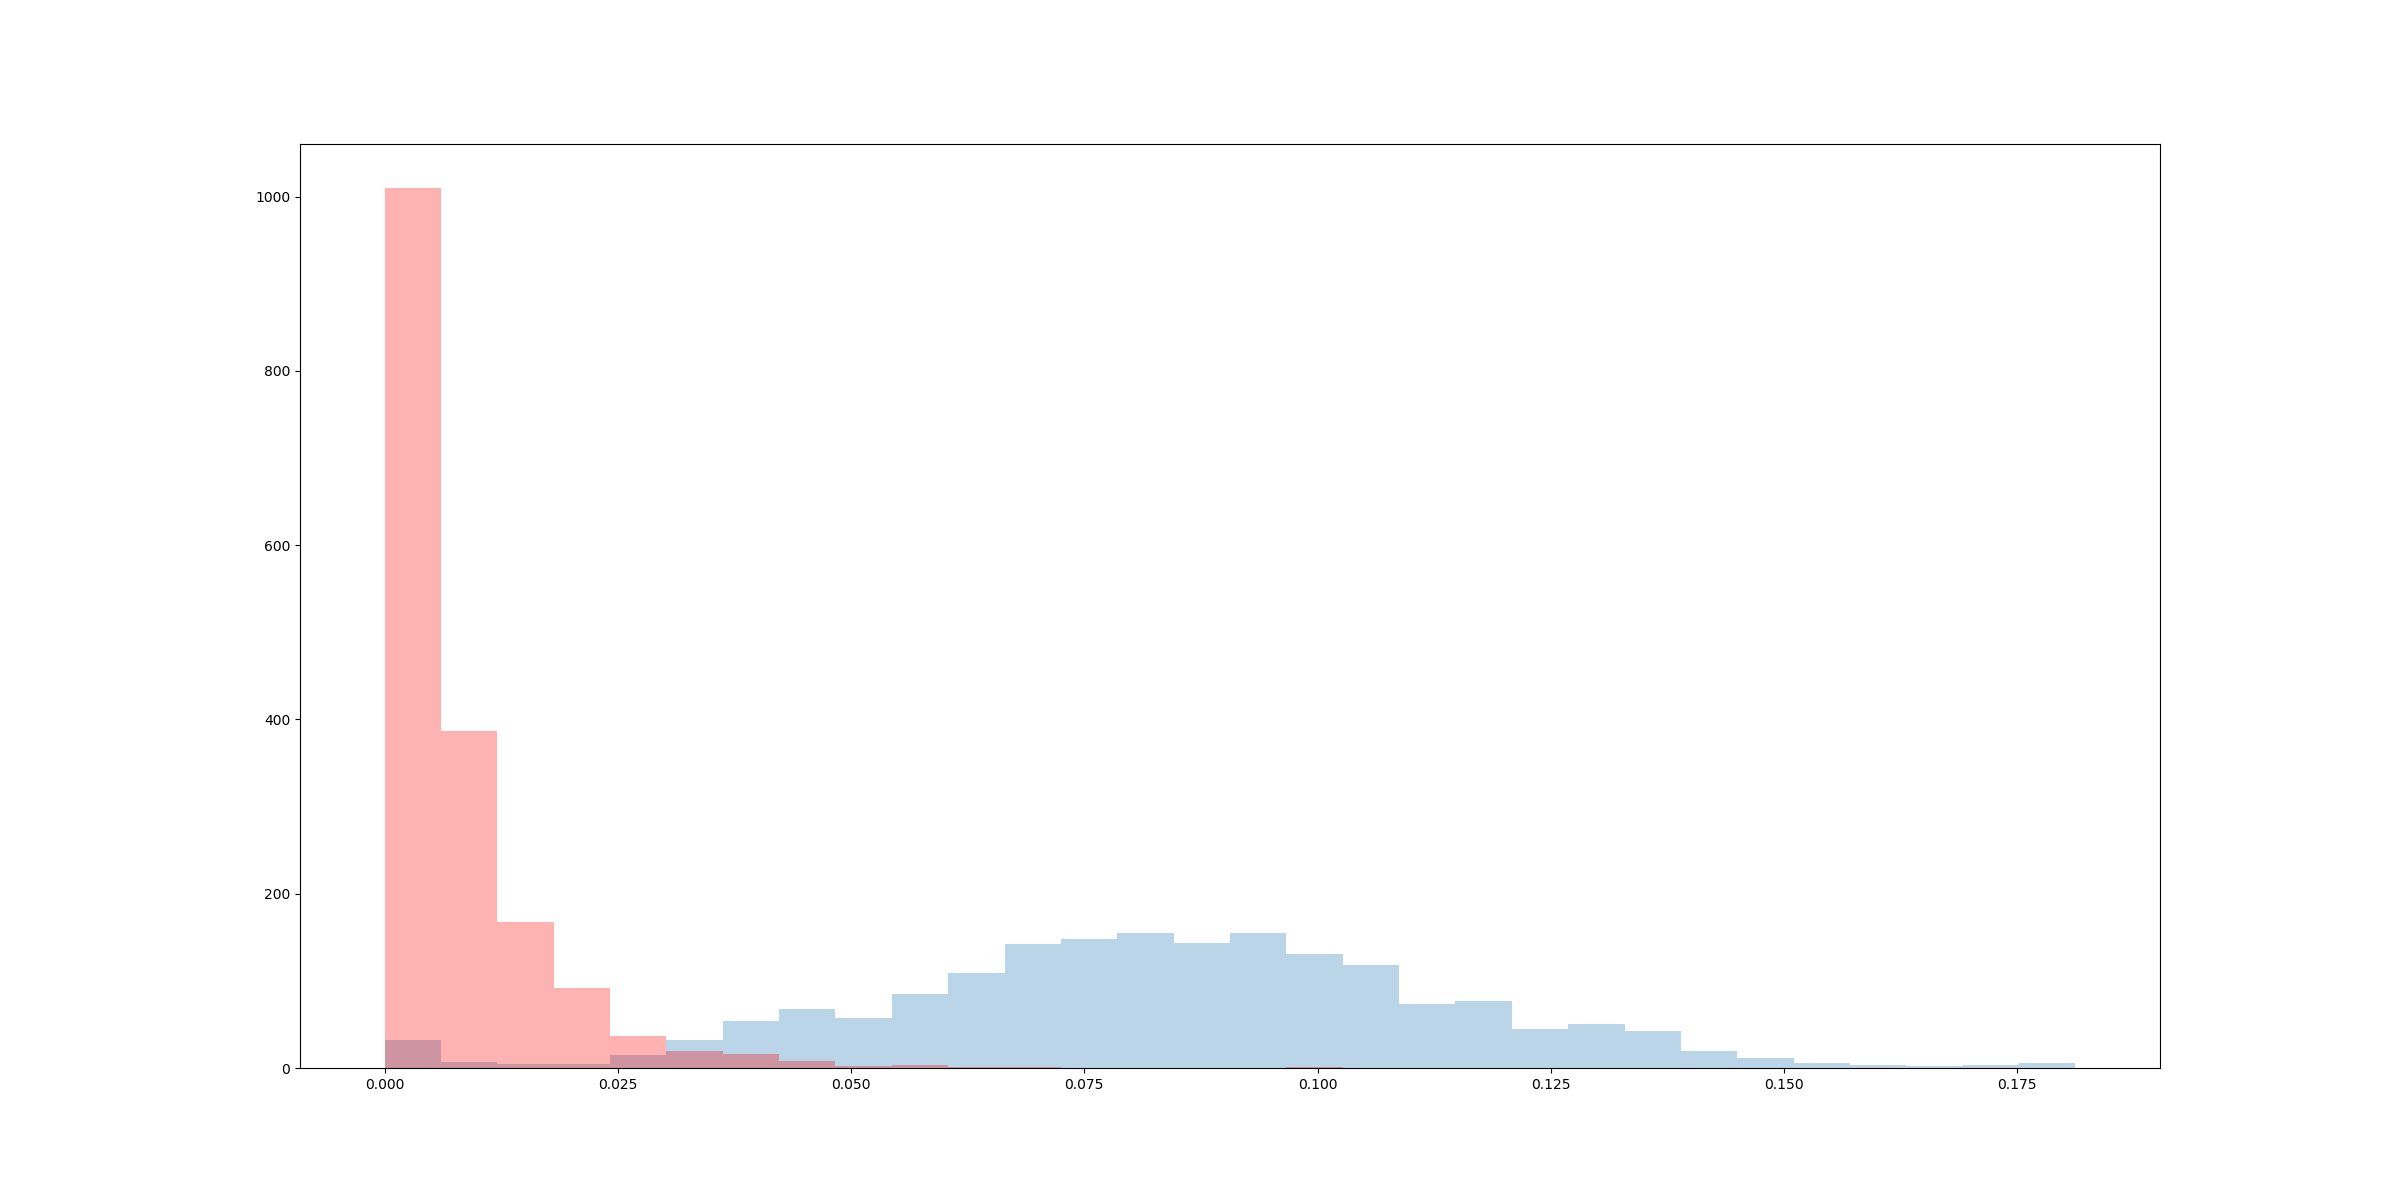
\includegraphics[trim=200 80 100 100, clip,width=.5\textwidth]{c3_figures/original_hist.png}
 \caption{Histogram of $0.7$-persistence of IGSM-based adversarial examples (red) and natural examples (blue) on MNIST. %The histogram shows that $0.7$-persistence for adversarial examples tends to be smaller than $0.7$-persistence for natural examples.
 }

 \label{fig:IGSMpersistenceMNIST}
 \end{figure}
\end{frame}
% Next, we investigate the relationship of network complexity and $(\gamma,\sigma)$-stability by revisiting the now classic work of \citet{szegedy2013} on adversarial examples. 

% Table \ref{table1} recreates and adds on to part of \cite[Table 1]{szegedy2013} in which networks of differing complexity are trained and attacked using L-BFGS. The table contains new columns showing the average $0.7$-persistence for both natural and adversarial examples for each network, as well as the average distortion for the adversarial examples. The distortion is the $\ell^2$-norm divided by square root of the dimension $n$. The first networks listed are of the form FC10-k, and are fully connected single layer ReLU networks that map each input vector $x \in \RR^{784}$ to an output vector $y \in \RR^{10}$ with a regularization added to the objective function of the form $\lambda\Norm{w}_2/N$, where $\lambda = 10^{-k}$ and $N$ is the number of parameters in the weight vector $w$ defining the network. The higher values of $\lambda$ indicate more regularization.  

% FC100-100-10 and FC200-200-10 are networks with 2 hidden layers (with 100 and 200 nodes, respectively) with regularization added for each layer of perceptrons with the $\lambda$ for each layer equal to $10^{-5}, 10^{-5}$, and  $10^{-6}$. Training for these networks was conducted with a fixed number of epochs (typically 21). For the bottom half of Table \ref{table1}, we also considered networks with four convolutional layers plus a max-pooling layer connected by ReLU to a fully connected hidden layer with increasing numbers of channels denoted as as ``C-Ch,'' where C reflects that this is a CNN and Ch denotes the number of channels. A more detailed description of these networks can be found in Appendix \ref{appendix:CNNs}.

\begin{frame}
  \frametitle{Experiments : MNIST Persistence vs Architecture}
 \begin{table}[ht]
 \centering
 \caption{Recreation of ~\citet{szegedy2013intriguing}, Table 1 for the MNIST dataset.  For each network, we show Testing Accuracy (in \%), Average Distortion ($\|x\|_2/\sqrt{n}$) of adversarial examples, and new columns show average $0.7$-persistence values for natural (Nat) and adversarial (Adv) images. 300 natural and 300 adversarial examples generated with L-BFGS were used for each aggregation.}
 \label{table1}
 \begin{tabular}{lllll}
 \toprule
 Network & Test Acc & Avg Dist & Persist (Nat) & Persist (Adv) \\
 \midrule
 FC10-4 & 92.09 & 0.123 & 0.93 & 1.68\\
 FC10-2 & 90.77 & 0.178 & 1.37 & 4.25\\
 FC10-0 & 86.89 & 0.278 & 1.92 & 12.22\\
 FC100-100-10 & 97.31 & 0.086 & 0.65 & 0.56 \\
 FC200-200-10 & 97.61 & 0.087 & 0.73 & 0.56 \\
 \midrule
 C-2 & 95.94 & 0.09 & 3.33 & 0.027 \\
 C-4 & 97.36 & 0.12 & 0.35 & 0.027 \\
 C-8 & 98.50 & 0.11 & 0.43  & 0.0517 \\
 C-16 & 98.90 & 0.11 & 0.53 & 0.0994 \\
 C-32 & 98.96 & 0.11 & 0.78 & 0.0836 \\
 C-64 & 99.00 & 0.10 & 0.81 & 0.0865 \\
 C-128 & 99.17 & 0.11 & 0.77 & 0.0883 \\
 C-256 & 99.09 & 0.11  & 0.83 & 0.0900 \\
 C-512 & 99.22 & 0.10 & 0.793 & 0.0929 \\

 \bottomrule
 \end{tabular}
 \end{table}
\end{frame}
% The main observation from Table \ref{table1} is that for higher complexity networks,
% adversarial examples tend to have smaller persistence than natural examples. Histograms reflecting these observations can be found in the supplemental material. %This can be seen as well in Figure \ref{fig:FC200-200-10}, which shows the $0.7$-persistence for natural and adversarial examples for the network FC200-200-10. 
% Another notable takeaway is that for models with fewer effective parameters, the attack distortion necessary to generate a successful attack is so great that the resulting image is often more stable than a natural image under that model, as seen particularly in the FC10 networks. Once there are sufficiently many parameters available in the neural network, we found that both the average distortion of the adversarial examples and the average $0.7$-persistence of the adversarial examples tended to be smaller. This observation is consistent with the idea that networks with more parameters are more likely to exhibit decision boundaries with more curvature.

\begin{frame}
  \frametitle{Experiments : ImageNet}

For ImageNet \citep{Imagenet-old}, we used pre-trained ImageNet classification models, including alexnet \citep{alexnet} and vgg16 \citep{simonyan2014very}.

% We then generated attacks based on the ILSVRC 2015 \citep{ILSVRC15}
% validation images for each of these networks using a variety of modern
% attack protocols, including Fast Gradient Sign Method (FGSM
% \citep{goodfellow_explaining_2014}), Momentum Iterative FGSM (MIFGSM
% \citep{dongMIFGSM}), Basic Iterative Method (BIM
% \citep{kurakin_adversarial_2016}), Projected Gradient Descent (PGD
% \citep{madry_towards_2017}), Randomized FGSM (R+FGSM
% \citep{tramer2018ensemble}), and Carlini-Wagner (CW
% ~\citet{carlini_towards_2016}). These were all generated using the
% TorchAttacks by \citet{kim2021torchattacks} toolset.

% \subsubsection{Investigation of $(\gamma, \sigma)$-stability on ImageNet}

% In this section, we show the results of Gaussian neighborhood sampling in ImageNet. Figures \ref{fig:imagenet_adv} and \ref{fig:persistent_interpimage} arise from vgg16 and adversarial examples created with BIM; results for other networks and attack strategies are similar, with additional figures in the supplementary material. Figure \ref{fig:imagenet_adv} (left) begins with an image $x$ with label \texttt{goldfinch}. For each equally spaced $\sigma\in(0,2)$, 100 i.i.d. samples were drawn from the Gaussian distribution $N(x,\sigma^2I)$, and the counts of the vgg16 classification for each label are shown. In Figure \ref{fig:imagenet_adv} (right), we see the same plot, but for an adversarial example targeted at the class \texttt{indigo\_bunting}, which is another type of bird, using the BIM attack protocol. %There are similar results with other attack protocols, as described in the supplementary materials.

% The key observation in Figure \ref{fig:imagenet_adv} is that the frequency of the class of the adversarial example (\texttt{indigo\_bunting}, shown in red) falls off much quicker than the class for the natural example (\texttt{goldfinch}, shown in black). In this particular example, the original class appears again after the adversarial class becomes less prevalent, but only for a short period of $\sigma$, after which other classes begin to dominate. In some examples the original class does not dominate at all after the decline of the adversarial class. The adversarial class almost never dominates for a long period of $\sigma$. 


 \begin{figure}[ht]
 \centering
 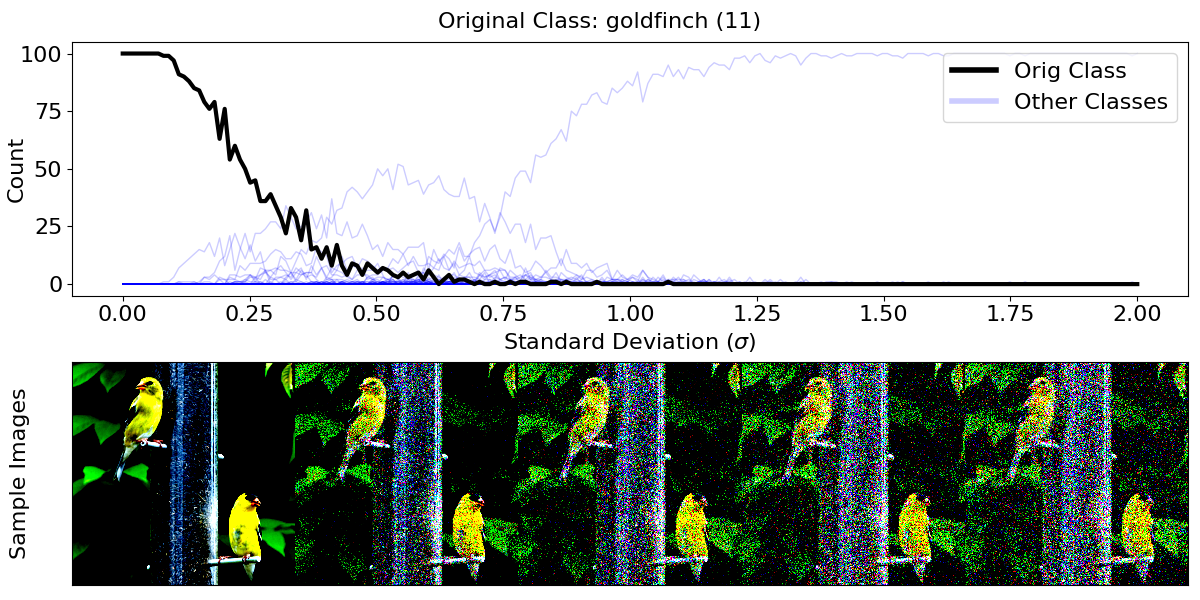
\includegraphics[width = .49\textwidth]{./c3_figures/ILSVRC2012_val_00001274-vgg16-sampling.png}
 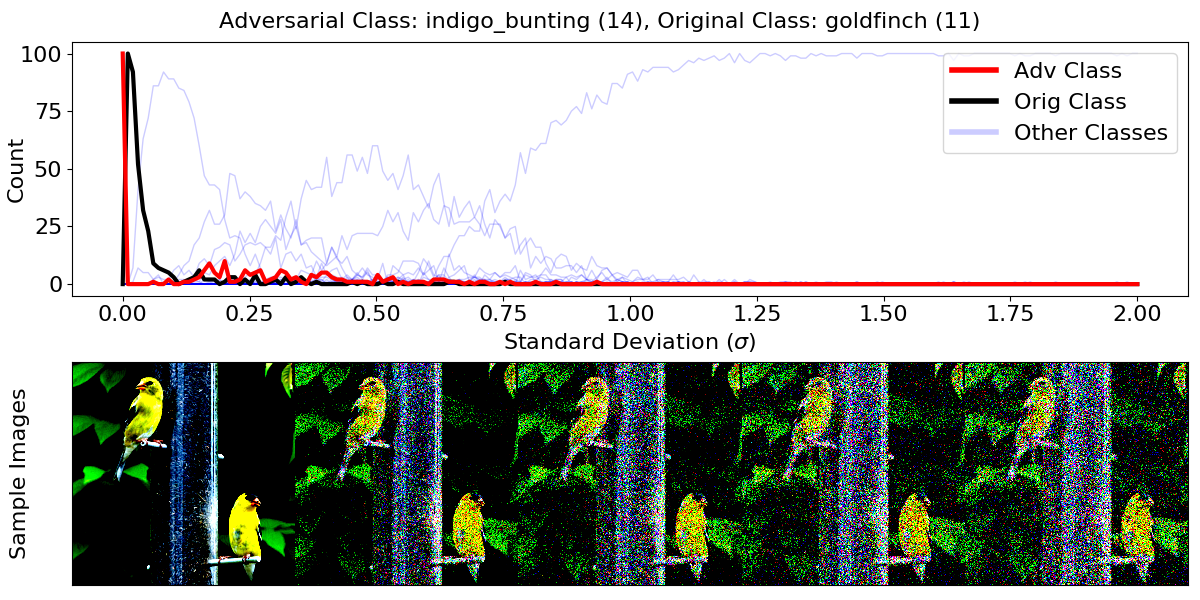
\includegraphics[width = .49\textwidth]{./c3_figures/IMNET-class-11-vgg16-BIM-48-attack_data-023.png}

 \caption{Frequency of each class in Gaussian samples with increasing variance around a \texttt{goldfinch} image (left) and an adversarial example of that image targeted at the \texttt{indigo\_bunting} class and calculated using the BIM attack (right). Bottoms show example sample images at different standard deviations for natural (left) and adversarial (right) examples.}
 \label{fig:imagenet_adv}
 \end{figure}
\end{frame}

% \subsubsection{Persistence of adversarial examples on ImageNet}

% Figure \ref{fig:persistent_interpimage} shows a plot of the $0.7$-persistence along the straight-line path between a natural example and adversarial example as parametrized between $0$ and $1$. It can be seen that the dropoff of persistence occurs precisely around the decision boundary. This indicates some sort of curvature favoring the class of the natural example, since otherwise the persistence would be roughly the same as the decision boundary is crossed.

\begin{frame}
  \frametitle{Experiments : ImageNet Persistence}
 \begin{figure}[ht]
 \centering
 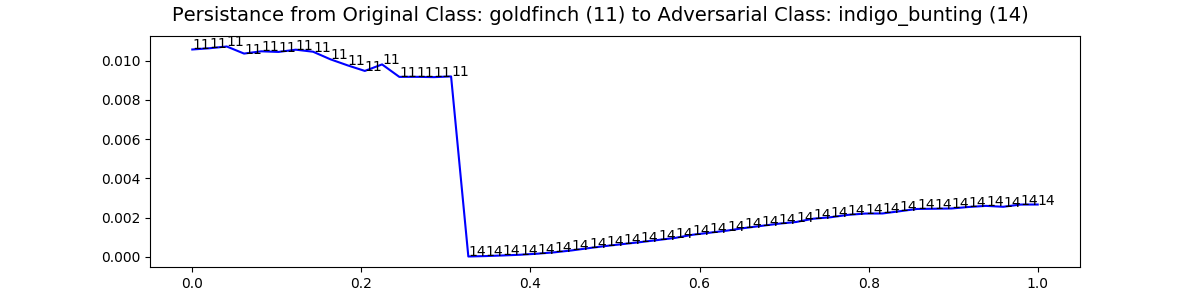
\includegraphics[width = \textwidth]
 {c3_figures/persistence_interpolation-IMNET-class-11-vgg16-BIM-48-attack_data-001.png}
 \caption{The $0.7$-persistence of images along the straight line path from an image in class \texttt{goldfinch} (11) to an adversarial image generated with BIM in the class \texttt{indigo\_bunting} (14) on a vgg16 classifier. The classification of each image on the straight line is listed as a number so that it is possible to see the transition from one class to another. The vertical axis is $0.7$-persistence and the horizontal axis is progress towards the adversarial image.}\label{fig:persistent_interpimage}
 \end{figure}
\end{frame}
% An aggregation of persistence for many randomly selected images from the \texttt{goldfinch} class in the validation set for Imagenet are presented in Table \ref{TAB:PersistenceAlexVGG}. 
% \begin{table}[!ht]
% \centering

% \begin{tabular}{llll}
% \toprule
% Network/Method & Avg Dist & Persist (Nat) & Persist (Adv) \\
% \midrule
% alexnet (total) & 0.0194 & 0.0155 & 0.0049 \\ 
% \:\: BIM        & 0.0188 & 0.0162 & 0.0050 \\ 
% \:\: MIFGSM     & 0.0240 & 0.0159 & 0.0053 \\ 
% \:\: PGD        & 0.0188 & 0.0162 & 0.0050 \\ 
% \midrule
% vgg16   (total) & 0.0154 & 0.0146 & 0.0011 \\ 
% \:\: BIM        & 0.0181 & 0.0145 & 0.0012 \\ 
% \:\: MIFGSM     & 0.0238 & 0.0149 & 0.0018 \\ 
% \:\: PGD        & 0.0181 & 0.0145 & 0.0012 \\ 
% \bottomrule
% \end{tabular}
% \caption{The $0.7$-persistence values for natural (Nat) and
%   adversarial (Adv) images along with average distortion for
%   adversarial images of alexnet and vgg16 for attacks generated with
%   BIM, MIFGSM, and PGD on images from class \texttt{goldfinch}
%   targeted toward other classes from the ILSVRC 2015 classification
%   labels.} \label{TAB:PersistenceAlexVGG}%\label{table:attack_pers} 
% \end{table}
% For each image of a \texttt{goldfinch} and for each network of alexnet and vgg16, attacks were prepared to a variety of 28 randomly selected targets using a BIM, MIFGSM, PGD, FGSM, R+FGSM, and CW attack strategies. The successful attacks were aggregated and their $0.7$-persistences were computed using the Bracketing Algorithm along with the $0.7$-persistences of the original images from which each attack was generated. Each attack strategy had a slightly different mixture of which source image and attack target combinations resulted in successful attacks. The overall rates for each are listed, as well as particular results on the most successful attack strategies in our experiments, BIM, MIFGSM, and PGD. The results indicate that adversarial images generated for these networks (alexnet and vgg16) using these attacks were less persistent, and hence less stable, than natural images for the same models. 

% \subsection{Decision Boundary Interpolation and Angle Measurement} \label{subsec:dbe}


\begin{frame}
  \frametitle{Experiments : Decision Boundary Angles}

 \begin{figure}[!ht]
 \centering\includegraphics[width=0.50\linewidth, trim=1.5cm 1.5cm 2cm 2cm, clip]{c3_figures/stab-mnist-C32-100-100-10-0.001-200-eval-1e-06-db_interp-angles-1stquadall199.png}\includegraphics[width=0.50\linewidth, trim=1.5cm 1.5cm 2cm 2cm, clip]{c3_figures/stab-mnist-C32-100-100-10-0.001-200-eval-1e-06-attack-db_interp-angles-1stquadall199.png}

 \caption{Decision boundary incident angles between test and test images (left) and between test and adversarial images (right). Angles (plotted Top) are referenced to decision boundary so $\pi/2$ radians (right limit of plots) corresponds with perfect orthogoonality to decision boundary. Lines and histograms measure angles of training gradients (Blue) linear interpolant (Black) and adversarial gradients (Red)}
 \label{fig:dba}
 \end{figure}
\end{frame}

% In order to understand this sudden drop in persistence across the decision boundary observed in Figure ~\ref{fig:persistent_interpimage}, we will investigate incident angle of the interpolation with the decision boundary. In order to measure these angles, we must first interpolate along the decision boundary between two points. We will do this for pairs of test and test and pairs of test and adversary. In both cases, we will use a bracketing algorithm along the interpolation from candidate points to identify a point within machine-precision of the decision boundary $x_b$. 

% Next, we will take 5000 samples from a Gaussian centered at this point with small standard deviation $\sigma = 10^{-6}$. Next, for each sample, we will perform an adversarial attack in order to produce a corresponding point on the opposite side of the decision boundary. Now for this new pair (sample and attacked sample), we will repeat the interpolation bracketing procedure in order to obtain the projection of this sample onto the decision boundary along the attack trajectory. Next, we will use singular value decomposition (SVD) on the differences between the projected samples and our decision boundary point $x_b$  to compute singular values and vectors from these projected samples. We will use the right singular vector corresponding with the smallest singular value as an approximation of a normal vector to the decision boundary at $x_b$. This point is difficult to compute due to degeneracy of SVD for small singular values, however in our tests, this value could be computed to a precision of 0.003. We will see that this level of precision exceeds exceeds that needed for the angles computed with respect to this normal vector sufficiently. 

% From Figure~\ref{fig:dba} we notice that neither training gradients nor adversarial gradients are orthogonal to the decision boundary. From a theory perspective, this is possible because this problem has more than 2 classes, so that the decision boundary includes $(0.34, 0.34, 0.32)$ and $(0.4, 0.4, 0.2)$. That is to say that the level set definition of the decision boundary has degrees of freedom that do not require orthogonality of gradients. More interestingly, both natural and adversarial linear interpolants tend to cross at acute angles with respect to the decision boundary, with adversarial attacks tending to be less acute. This suggests that adversaries are exploiting the obliqueness of the decision boundary with respect to test points. We will leverage this understanding with manifold alignment to see if constraining gradients to a lower dimensional manifold, and thus increasing orthogonality of gradients will increase robustness. 

% \subsection{Manifold Alignment on MNIST via PCA} \label{subsec:mae}

% In order to provide an empirical measure of alignment, we first require a well defined image manifold.
% The task of discovering the true structure of \textit{k}-dimensional manifolds in $\mathds{R}^d$ given a set of points sampled on the manifold has been studied previously \citep{khoury2018}.
% Many algorithms produce solutions which are provably accurate under data density constraints.
% Unfortunately, these algorithms have difficulty extending to domains with large $d$ due to the curse of dimensionality.
% Our solution to this fundamental problem is to sidestep it entirely by redefining our dataset.
% We begin by projecting our data onto a well known low dimensional manifold, which we can then measure with certainty.
% \begin{figure}[h]
% \begin{center}
%     % \fbox{\rule[-.5cm]{0cm}{4cm} \rule[-.5cm]{4cm}{0cm}}

%     \includegraphics[width=0.8\linewidth]{c3_figures/manifold_model_cosine_hist.png}
%     \includegraphics[width=0.8\linewidth]{c3_figures/robust_model_cosine_hist.png}
% \end{center}
%     \caption{Comparison of on-manifold components between baseline network, robust trained models, and manifold optimized models. Large values indicate higher similarity to the manifold. Both robust and manifold optimized models are more 'on-manifold' than the baseline, with adversarial training being slightly less so.}
%     \label{fig:hist_cosine}
% \end{figure}

% \begin{figure}[h]
%     \centering
%     \includegraphics[width=0.8\linewidth]{c3_figures/FGSM_attacks_accuracy_known_manifold.png}
%     \includegraphics[width=0.8\linewidth]{c3_figures/PGD_attacks_accuracy_known_manifold.png}
%     \caption{Comparison of adversarial robustness for PMNIST models under various training conditions. For both FGSM and PGD, we see a slight increase in robustness from using manifold optimization. Adversarial training still improves performance significantly more than manifold optimization. Another observation to note is that when both the manifold, and adversarial objective were optimized, increased robustness against FGSM attacks was observed. All robust models were trained using the $l_\infty$ norm at epsilon = 0.1.}
%     \label{fig:model_robustness}
% \end{figure}

% We first fit a PCA model on all training data, using $k$ components for each class, where $k << d$.
% Given the original dataset $X$, we create a new dataset $X_{\mathcal{M}} := \{x \times \textbf{W}^T \times \textbf{W} : x \in X \}$.
% We will refer to this set of component vectors as $\textbf{W}$.
% Because the rank of the linear transformation matrix, $k$, is defined lower than the dimension of the input space, $d$, this creates a dataset which lies on a linear subspace of $\mathds{R}^d$.
% This subspace is defined by the span of $X \times \textbf{W}^T$ and any vector in $\mathds{R}^d$ can be projected onto it.
% Any data point drawn from $\{z \times \textbf{W}^T : z \in \mathds{R}^k \}$ is considered a valid datapoint.
% This gives us a continuous linear subspace which can be used as a data manifold.

% Given that it our goal to study the simplest possible case, we chose MNIST as the dataset to be projected and selected $k = 28$ components.
% We refer to this new dataset as Projected MNIST (PMNIST).
% The true rank of PMNIST is lower than that of the original MNIST data, meaning there was information lost in this projection.
% The remaining information we found is sufficient to achieve 92\% accuracy using a baseline Multylayer Perceptron (MLP), and the resulting images retain their semantic properties as shown in Figure \ref{fig:perception}.

% \begin{figure*}
%     \centering
%     \includegraphics[width=0.25\linewidth]{c3_figures/pag_0.png}
%     \includegraphics[width=0.25\linewidth]{c3_figures/pag_1.png}
%     \includegraphics[width=0.25\linewidth]{c3_figures/pag_2.png}
%     \caption{Visual example of manifold optimized model transforming 2 into 3. Original PMNIST image on left, center image is center point between original and attacked, on right is the attacked image. Transformation performed using PGD using the $l_\infty$ norm. Visual evidence of manifold alignment is often subjective and difficult to quantify. This example is provided as a baseline to substantiate our claim that our empirical measurements of alignment are valid.}
%     \label{fig:perception}
% \end{figure*}

% Where $L(\theta, x, y)$ represents our classification loss term and $\alpha$ is a hyper parameter determining the weight of the manifold loss term.

% \subsection{Manifold Aligned Gradients} \label{subsec:ma}

% Component vectors extracted from the original dataset are used to project gradient examples onto our pre-defined image manifold.

% Given a gradient example $\nabla_x = \frac{\partial f_\theta(x, y)}{\partial x}$ where $f_\theta$ represents a neural network parameterized by weights $\theta$. $\nabla_x$ is transformed using the coefficient vectors \textbf{W}.

% \begin{equation}
%     \rho_x = \nabla_x \times \textbf{W}^T \times \textbf{W}    
% \end{equation}
% The projection of the original vector onto this new transformed vector we will refer to as $P_{\mathcal{M}}$.
% The norm of this projection gives a metric of manifold alignment.
% \begin{equation}
%     \frac{|| \nabla_x || }{||P_{\mathcal{M}}(\nabla_x )||}
%   \label{equ:ratio}
% \end{equation}
% This gives us a way of measuring the ratio between on-manifold and off-manifold components of the gradient.
% Additionally, both cosine similarity and the vector rejection were also tested but the norm ratio we found to be the most stable in training.
% We use this measure as both a metric and a loss, allowing us to optimize the following objective.
% \begin{equation}
%   \mathds{E}_{(x,y) \sim \mathcal{D}} \left[ L(\theta, x,y)  + \alpha \frac{|| \nabla_x || }{||P_{\mathcal{M}}(\nabla_x )||} \right]
%   \label{equ:loss}
% \end{equation}

% \subsection{Manifold Alignment Robustness Results}

% All models were two layer MLPs with 1568 nodes in each hidden layer.
% The hidden layer size was chosen as twice the input size.
% This arrangement was chosen to maintain the simplest possible case.

% Two types of attacks were leveraged in this study: fast gradient sign method (FGSM) \citep{goodfellow_explaining_2014} and projected gradient descent (PGD) \citep{madry_towards_2017}.
% A total of four models were trained and evaluated on these attacks: Baseline, Robust, Manifold and Manifold Robust.
% All models, including the baseline, were trained on PMNIST.
% ``Robust" in our case refers to adversarial training.
% All robust models were trained using the $l_\infty$ norm at $\epsilon = 0.1$.
% Manifold Robust refers to both optimizing our manifold objective and robust training simultaneously.

% Figure \ref{fig:hist_cosine} shows the cosine similarity on the testing set of PMNIST for both the Manifold model and Robust model.
% Higher values indicate the model is more aligned with the manifold.
% Both models here are shown to be more on manifold than the Baseline.
% This demonstrates that our metric for alignment is being optimized as a consequence of adversarial training.

% Figure \ref{fig:model_robustness} shows the adversarial robustness of each model.
% In both cases, aligning the model to the manifold shows an increase in robustness over the baseline.
% However, we do not consider the performance boost against PGD to be significant enough to call these models robust against PGD attacks.
% Another point of interest that while using both our manifold alignment metric and adversarial training, we see an even greater improvement against FGSM attacks.

% The fact that this performance increase is not shared by PGD training may indicate a relationship between these methods.
% Our current hypothesis is that a linear representation of the image manifold is sufficient to defend against linear attacks such as FGSM, but cannot defend against a non-linear adversary.

% \section{Conclusion}

% In order to better understand the observed tendency for points near natural data to be classified similarly and points near
% adversarial examples to be classified differently, we defined a notion of $(\gamma,\sigma)$-stability which is easily estimated by Monte Carlo sampling. For any data point $x$, we then define the $\gamma$-persistence to to be the smallest $\sigma_\gamma$ such that the probability of similarly classified data is at least $\gamma$ when sampling from Gaussian distributions with mean $x$ and standard deviation less than $\sigma_\gamma$. The persistence value can be quickly estimated by a Bracketing Algorithm. These two measures were considered with regard to both the MNIST and ImageNet datasets and with respect to a variety of classifiers and adversarial attacks. We found that adversarial examples were much less stable than natural examples in that the $0.7$-persistence for natural data was usually significantly larger than the $0.7$-persistence for adversarial examples. We also saw that the dropoff of the persistence tends to happen precisely near the decision boundary. Each of these observations is strong evidence toward the hypothesis that adversarial examples exploit oblique structure of overlapping decision boundaries around the adversarial class, whereas natural images lie outside such regions.In addition, we found that some adversarial examples may be more stable than others, and a more detailed probing using the concept of $(\gamma,\sigma)$-stability and the $\gamma$-persistence statistic may be able to help with a more nuanced understanding of the geometry and obliqueness of the boundary.

% We reinforced this obliqueness hypothesis by computing angles of linear interpolants with respect to the decision boundary, showing that most interpolants cross the decision boundary between classes at very shallow angles. Furthermore, adversarial interpolants tend to cross at less shallow, but still acute angles. Furthermore, we present the simplest possible case of our hypothesis that manifold alignment implies adversarial robustness.
% Extending this to show results on more complex models and datasets is left to future work.
% In this early work, we only test against a linear manifold and show that it provides robustness against FGSM.
% We conclude that training a model to be aligned with a low dimensional manifold on which your data lies is related to robust training.
% While this model shows some properties of adversarial robustness, it is still vulnerable to PGD attacks.
% Additionally, a model trained to be robust using adversarial training shows manifold alignment under our definition.

% \nocite{langley00}


% \section{Conclusion}

% In order to better understand the observed tendency for points near natural data to be classified similarly and points near
% adversarial examples to be classified differently, we defined a notion of $(\gamma,\sigma)$-stability which is easily estimated by Monte Carlo sampling. For any data point $x$, we then define the $\gamma$-persistence to to be the smallest $\sigma_\gamma$ such that the probability of similarly classified data is at least $\gamma$ when sampling from Gaussian distributions with mean $x$ and standard deviation less than $\sigma_\gamma$. The persistence value can be quickly estimated by a Bracketing Algorithm. These two measures were considered with regard to both the MNIST and ImageNet datasets and with respect to a variety of classifiers and adversarial attacks. We found that adversarial examples were much less stable than natural examples in that the $0.7$-persistence for natural data was usually significantly larger than the $0.7$-persistence for adversarial examples. We also saw that the dropoff of the persistence tends to happen precisely near the decision boundary. Each of these observations is strong evidence toward the hypothesis that adversarial examples arise inside cones or high curvature regions in the adversarial class, whereas natural images lie outside such regions.

% We also found that often the most likely class for perturbations of an adversarial examples is a class other than the class of the original natural example used to generate the adversarial example; instead, some other background class is favored. In addition, we found that some adversarial examples may be more stable than others, and a more detailed probing using the concept of $(\gamma,\sigma)$-stability and the $\gamma$-persistence statistic may be able to help with a more nuanced understanding of the geometry and curvature of the decision boundary. Although not pursued here, the observations and statistics used in this paper could potentially be used to develop methods to detect adversarial examples as in \citep{crecchi2019,frosst2018,hosseini2019odds,Lee2018ASU,qin2020,roth19aodds} and others. As with other methods of detection, this may be susceptible to adaptive attacks as discussed by ~\citet{tramer2020adaptive}. 

\begin{frame}
  \frametitle{Conclusions}
  \begin{itemize}
    \item Geometric properties including curvature and alignment to
      decision boundaries seem to be related with robustness.
      \item Direct computation of these geometric properties is
        expensive and at odds with the fact that much greater scale is
        needed to understand these properties in practice.
        \item We could benefit from faster methods to analyze
          geometric properties from models -- Monte Carlo is what you
          do when you can't solve your differential equations by
          faster means!
          \item Decision boundaries are askew from interpolation
            between natural images!
          \end{itemize}
        \end{frame}

  % Persistence
% carefully pose some definitions for adversarial examples
% develop persistence metric and talk about how it is used


% EPK
% carefully walk through EPK definition and proof
% use diagram as an aide to illustrate major issues
% main takewaways reduction to a single kernel is not practical
% there is lots of potential to use this phrasing to do decompositions
%and understand the geometry.
% many remarks

\section{An Exact Kernel Equivalence for Finite Classification Models} % Main chapter title
\label{Chapter4} % For referencing the chapter elsewhere, use \ref{Chapter1} 

% This paper proposes the first exact path kernel representation for
% general gradient trained classifiers. The primary derivation and proof
% was written by Brian Bell and the supporting impoementation and work
% were mostly conducted by Michael Geyer. The central focus of the paper
% is on the derivation and demonstration that this method works in
% practice. The interest that gave rise for this approach comes from the fact that
% kernel methods and more specifically bilinear map based models
% decompose their predictions into a contribution from each of their
% training data. the Neural Tangent Kernel (NTK) is an interesting tool,
% but predicated on too many approximation assumptions. This exact
% formulation allows a much more solid foundation for analyzing neural
% networks and suggests the possibility that predictions can be
% decomposed using this framework. The implementation and application of
% this method to real machine-learning models and tasks demonstrates
% that it is not only a theoretical framework, it is practical! This
% paper was accepted at the Topology Algebra and Geometry (TAG) workshop
% at ICML 2023 (an archival publication).  

% \section{Introduction}

% This study investigates the relationship between kernel methods and finite parametric models. To date, interpreting the predictions of complex models, like neural networks, has proven to be challenging. Prior work has shown that the inference-time predictions of a neural network can be exactly written as a sum of independent predictions computed with respect to each training point. We formally show that classification models trained with cross-entropy loss can be exactly formulated as a kernel machine. It is our hope that these new theoretical results will open new research directions in the interpretation of neural network behavior.




% % \begin{tikzpicture}[scale=0.8]
% % % main step angles
% % \def\angA{72}
% % \def\angB{35}
% % \def\angC{15}
% % \def\angD{-20}

% % \def\nang{62}
% % \def\dang{45}
% % \def\sang{15}
% % \def\pang{30}

% % % \def\mang{29}
% % % \def\sang{39}
% % % \def\tang{50}
% % % \def\bang{60}
% % % \def\dang{34}

% %   \def\xs{1.0}
% %   \def\xa{4}
% %   \def\xe{1.0}
% %   \def\xd{0.75}
% %   \def\xn{0.5}
% %   \def\xi{1.4}
% %   % incoming edge
% %   \coordinate  (s1) at (0,0);
% %   \coordinate  (si1) at ($ (s1) + (\angA:1) $);
% %   \coordinate  (s2) at ($ (si1) + (\angA:\xs) $);
% %   \coordinate  (s3) at ($ (s2) + (\angB:\xa) $);
% %   \coordinate  (si3) at ($(s3) + (\angC:\xs) $);
% %   \coordinate  (s4) at ($(si3) + (\angC:\xs) $);

% %   %\node[fill=black,circle,inner sep=1.9] (s01) at (s1) {};
% %   \path (si1) -- (s2) node [midway, sloped] (elip) {\ldots};
% %   \path (s3) -- (si3) node [midway, sloped] (elip) {\ldots};
% %   \node[fill=black,circle,inner sep=1.9] (s01) at (s1) {};
% %   \node[fill=black,circle,inner sep=1.9] (s02) at (s2) {};
% %   \node[fill=black,circle,inner sep=1.9] (s03) at (s3) {};
% %   \node[fill=black,circle,inner sep=1.9] (s04) at (s4) {};
% %   %\node[fill=black,circle,inner sep=1.9] (s04) at (s4) {};

% % \draw[name path=pb, black, line width=0.4mm, draw opacity=0.7] (s2) -- (s3);
% % \draw[black, line width=0.4mm, draw opacity=0.7] (s1) -- (si1);
% % \path[name path=fb, black, line width=0.4mm, draw opacity=0.7] (s1) -- (s2);
% % \draw[name path=gb, black, line width=0.4mm, draw opacity=0.7] (si3) -- (s4);

% % \coordinate (p1) at (s2);%($ (s2)+(\ang:\xi) $);   % origin
% % % \coordinate (p1n) at ($ (p1)+(\nang:\xe) $);       % ntk test

% % % \coordinate (p1d) at ($ (p1)+(\angB+\sang:\xe) $); % dpk test

% % % \coordinate (p1e) at ($ (p1)+(\angB+\sang:\xe) $); % epk test
% % % \coordinate (p1t) at ($ (p1)+(\angD:\xe) $); % ntk train
% % % \coordinate (p1b) at ($ (p1)+(\angB:\xe) $); % dpk epk train

% % % \coordinate (p2) at  ($ (p1b)+(\angB:\xi) $);   % origin
% % % \coordinate (p2n) at ($ (p2)+(\nang:\xe) $);       % ntk test
% % % \coordinate (p2d) at ($ (p2)+(\angB+\sang:\xe) $); % dpk test
% % % \coordinate (p2e) at ($ (p2)+(\angB+\pang:\xe) $); % epk test
% % % \coordinate (p2t) at ($ (p2)+(\angD:\xe) $); % ntk train
% % % \coordinate (p2b) at ($ (p2)+(\angB:\xe) $); % dpk epk train

% % % \coordinate (p3) at  (s4); %($ (s4)+(\angB:\xi) $);   % origin
% % %   \draw[line width=10pt, ->, red] (0,0) -- (3,0);
% % %   \draw[line width=10pt, ->, blue] (0,0.5) -- (3,0.5);
  
% % %     \begin{scope}
% % %     \clip (-1,0) rectangle (3,1);
% % %     \draw[line width=10pt, ->] (0,0) -- (3,0);
% % %   \end{scope}
% % % \coordinate (p3n) at ($ (p3)+(\nang:\xe) $);       % ntk test
% % % \coordinate (p3d) at ($ (p3)+(\nang:\xe) $); % dpk test
% % % \coordinate (p3e) at ($ (p3)+(\nang:\xe) $); % epk test
% % % \coordinate (p3t) at ($ (p3)+(\angD:\xe) $); % ntk train
% % % \coordinate (p3b) at ($ (p3)+(\angD:\xe) $); % dpk epk train

% % % \coordinate (p2) at ($ (p1a)+(\angB:0.6) $);
% % % \coordinate (p2a) at ($ (p2)+(\angB:\xe) $);
% % % \coordinate (p2b) at ($ (p2)+(\sang:\xe) $); 
% % % \coordinate (p3) at ($ (p2a)+(\angB:\xi) $);
% % % \coordinate (p3a) at ($ (p3)+(\angB:\xe) $);
% % % \coordinate (p3b) at ($ (p3)+(\tang:\xe) $);
% % % \coordinate (n0) at ($ (s1)+(\nang:\xn) $);
% % % \coordinate (n1) at ($ (p1)+(\nang:\xn) $);
% % % \coordinate (n2) at ($ (p2)+(\nang:\xn) $);
% % % \coordinate (n3) at ($ (p3)+(\nang:\xn) $);
% % % \coordinate (d0) at ($ (s1)+(\dang:\xd) $);
% % % \coordinate (d1) at ($ (p1)+(\dang:\xd) $);
% % % \coordinate (d2) at ($ (p2)+(\dang:\xd) $);
% % % \coordinate (d3) at ($ (p3)+(\dang:\xd) $);
    
% % % \draw[vector, ->, ntk] (s1) -- (n0) node[scale=1,above left=-3mm and 3mm, draw opacity=0.5] {$\vu{x}$};
% % % \draw[vector, ->, dpk] (s1) -- (d0) node[scale=1,above left=-3mm and 3mm, draw opacity=0.5] {$\vu{x}$};
% % % \draw[vector, opacity=0.5, ->, ntk] (p1) -- (p1n) node[scale=1,above left=-3mm and 3mm, draw opacity=0.2] {};%ntk test};

% % % \draw[vector, opacity=0.5,  ->, dpk] (p1) -- (p1d) node[scale=1,above left=-3mm and 3mm, draw opacity=0.2] {};%dpk test};

% % % \begin{scope}
% % % \clip (p1) -- (p1d) -- ($(p1d) + (0,1) $) -- ($ (p1) + (-1,1) $);
% % % \draw[vector, ->, epk] (p1) -- (p1e) node[scale=1,above left=-3mm and 3mm, draw opacity=0.2] {};%epk test};
% % % \end{scope}
% % % \draw[vector, ->, ntk] (p1) -- (p1t) node[scale=1,above left=-3mm and 3mm, draw opacity=0.2] {};%ntk train};
% % % \draw[vector, ->, epk] (p1) -- (p1b) node[scale=1,above left=-3mm and 3mm, draw opacity=0.2] {};%(de)pk test};

% % % \draw[vector, ->, ntk] (p2) -- (p2n) node[scale=1,above left=-3mm and 3mm, draw opacity=0.2] {};%ntk test};
% % % \draw[vector, ->, dpk] (p2) -- (p2d) node[scale=1,above left=-3mm and 3mm, draw opacity=0.2] {};%dpk test};
% % % \draw[vector, ->, epk] (p2) -- (p2e) node[scale=1,above left=-3mm and 3mm, draw opacity=0.2] {};%epk test};
% % % \draw[vector, ->, ntk] (p2) -- (p2t) node[scale=1,above left=-3mm and 3mm, draw opacity=0.2] {};%ntk train};
% % % \draw[vector, ->, epk] (p2) -- (p2b) node[scale=1,above left=-3mm and 3mm, draw opacity=0.2] {};%(de)pk test};



% % % \draw[vector, ->, ntk] (p3) -- (p3n) node[scale=1,above left=-3mm and 3mm, draw opacity=0.2] {};%ntk test};
% % % \draw[vector, ->, dpk] (p3) -- (p3d) node[scale=1,above left=-3mm and 3mm, draw opacity=0.2] {};%dpk test};
% % % \draw[vector, ->, epk] (p3) -- (p3e) node[scale=1,above left=-3mm and 3mm, draw opacity=0.2] {};%epk test};
% % % \draw[vector, ->, ntk] (p3) -- (p3t) node[scale=1,above left=-3mm and 3mm, draw opacity=0.2] {};%ntk train};
% % % \draw[vector, ->, epk] (p3) -- (p3b) node[scale=1,above left=-3mm and 3mm, draw opacity=0.2] {};%(de)pk test};

% % \draw [name path=pa, thick , ->]
% %   (p1) .. controls ($ (s2) + (37:2.1) $)  .. ($ (s3) + (125:0.6) $);
% %   \draw [name path=fa, thick , ->]
% %   (s1) .. controls ($ (s1) + (80:1.1) $)  .. ($ (s2) + (162:0.50) $);
% %   \draw [name path=ga, thick , ->]
% %   (s3) .. controls ($ (s3) + (20:1) $)  .. ($ (s4) + (105:0.4) $);
% % \tikzfillbetween[of=pa and pb]{orange, opacity=0.2};
% % \tikzfillbetween[of=fa and fb]{orange, opacity=0.2}; 
% % \tikzfillbetween[of=ga and gb]{orange, opacity=0.2};

% % % \draw[vector, ->, epk] (p1) -- (p1b) node[scale=1,above left=-3mm and 3mm, draw opacity=0.5] {$\vu{x}$};
% % % \draw[vector, ->, epk] (p1) -- (p1a) node[scale=1,below left=1mm and 0mm, draw opacity=0.5] {$\vu{y}$};
% % % \draw[vector, ->, epk] (p2) -- (p2b) node[scale=1,above left=-3mm and 3mm, draw opacity=0.5] {$\vu{x}$};
% % % \draw[vector, ->, epk] (p2) -- (p2a) node[scale=1,below left=1mm and 0mm, draw opacity=0.5] {$\vu{y}$};
% % % \draw[vector, ->, epk] (p3) -- (p3b) node[scale=1,above left=-3mm and 3mm, draw opacity=0.5] {$\vu{x}$};
% % % \draw[vector, ->, epk] (p3) -- (p3a) node[scale=1,below left=1mm and 0mm, draw opacity=0.5] {$\vu{y}$};

% % \end{tikzpicture}

\begin{frame}
\frametitle{Model Optimization Step}  
\begin{figure}[!ht]
\centering
\begin{tikzpicture}[scale=1.2]
\def\bang{72}
\def\ang{35}
\def\lang{15}
\def\mang{57}
\def\sang{69}
\def\kang{90}
\def\tang{87}
\def\dang{34}
\def\xs{1.0}
\def\xa{4}
\def\xe{1.0}
\def\xd{0.75}
\def\xn{0.5}
\def\xi{0.4}
% incoming edge
\coordinate  (s1) at (0,0);
\coordinate  (si1) at ($ (s1) + (\bang:1) $);
\coordinate  (s2) at ($ (si1) + (\bang:\xs) $);
\coordinate  (s3) at ($ (s2) + (\ang:\xa) $);
\coordinate  (si3) at ($(s3) + (\lang:\xs) $);
\coordinate  (s4) at ($(si3) + (\lang:\xs) $);

%\node[fill=black,circle,inner sep=1.9] (s01) at (s1) {};
\path (si1) -- (s2) node [midway, sloped] (elip) {\ldots};
\path (s3) -- (si3) node [midway, sloped] (elip) {\ldots};
\node[fill=black,circle,inner sep=1.9] (s01) at (s1) {};
\node [below right=0mm and 1mm, rotate=\kang-90] (ss1) at (s01) {$w_1(t=0)$};
\node[fill=black,circle,inner sep=1.9] (s02) at (s2) {};
\node [below right=0mm and 1mm, rotate=\kang-90] (ss2) at (s02) {$w_s(t=0)$};
\node[fill=black,circle,inner sep=1.9] (s03) at (s3) {};
\node [below right=-1mm and 1mm, rotate=\kang-90] (ss3) at (s3) {$w_s(t=1)=w_{s+1}(t=0)$}; 
\node[fill=black,circle,inner sep=1.9] (s04) at (s4) {};
%\node[fill=black,circle,inner sep=1.9] (s04) at (s4) {};
\node [below right=-2mm and 1mm, rotate=\kang-90] (ss4) at (s04) {$w_S(t=0)$};
\draw[black, line width=0.4mm, draw opacity=0.3] (s2) -- (s3);
\draw[black, line width=0.4mm, draw opacity=0.3] (s1) -- (si1);
\draw[black, line width=0.4mm, draw opacity=0.3] (si3) -- (s4);

\coordinate (p1) at (s2);%($ (s2)+(\ang:\xi) $);
\coordinate (p1a) at ($ (p1)+(\ang:\xe) $);
\coordinate (p1b) at ($ (p1)+(\mang:\xe) $);
\coordinate (p2) at ($ (p1a)+(\ang:0.6) $);
\coordinate (p2a) at ($ (p2)+(\ang:\xe) $);
\coordinate (p2b) at ($ (p2)+(\sang:\xe) $); 
\coordinate (p2c) at ($ (p2)+(\mang:\xe) $); 
\coordinate (p3) at ($ (p2a)+(\ang:\xi) $);
\coordinate (p3a) at ($ (p3)+(\ang:\xe) $);
\coordinate (p3b) at ($ (p3)+(\tang:\xe) $);
\coordinate (p3c) at ($ (p3)+(\mang:\xe) $);
\coordinate (n0) at ($ (s1)+(\bang:\xn) $);
\coordinate (n1) at ($ (p1)+(\bang:\xn) $);
\coordinate (n2) at ($ (p2)+(\bang:\xn) $);
\coordinate (n3) at ($ (p3)+(\bang:\xn) $);
\coordinate (d0) at ($ (s1)+(\dang:\xd) $);
\coordinate (d1) at ($ (p1)+(\dang:\xd) $);
\coordinate (d2) at ($ (p2)+(\dang:\xd) $);
\coordinate (d3) at ($ (p3)+(\dang:\xd) $);

\draw[name path=pb, black, line width=0.4mm, draw opacity=0.7] (s2) -- (s3);
\draw[black, line width=0.4mm, draw opacity=0.7] (s1) -- (si1);
\path[name path=fb, black, line width=0.4mm, draw opacity=0.7] (s1) -- (s2);
\draw[name path=gb, black, line width=0.4mm, draw opacity=0.7] (si3) -- (s4);  
  \draw [name path=pa, thick , ->, opacity=0.0]
  (p1) .. controls ($ (s2) + (37:2.1) $)  .. ($ (s3) + (125:0.6) $);
  \draw [name path=fa, thick , ->, opacity=0.0]
  (s1) .. controls ($ (s1) + (80:1.1) $)  .. ($ (s2) + (162:0.50) $);
  \draw [name path=ga, thick , ->, opacity=0.0]
  (s3) .. controls ($ (s3) + (20:1) $)  .. ($ (s4) + (105:0.4) $);
\tikzfillbetween[of=pa and pb]{orange, opacity=0.2};
\tikzfillbetween[of=fa and fb]{orange, opacity=0.2}; 
\tikzfillbetween[of=ga and gb]{orange, opacity=0.2};
    
% \draw[vector, ->, ntk] (s1) -- (n0) node[scale=1,above left=-3mm and 3mm, draw opacity=0.5] {$\vu{x}$};
% \draw[vector, ->, dpk] (s1) -- (d0) node[scale=1,above left=-3mm and 3mm, draw opacity=0.5] {$\vu{x}$};
\draw[vector, ->, dpk] (p1) -- (p1b) node[scale=1,above left=-5mm and 2mm, draw opacity=0.5] {$\nabla f_{w_s(t=0)}(x)$};
\begin{scope}
\clip (p1) -- (p1b) -- ($(p1b) + (90+\mang:0.1) $) -- ($ (p1) + (90+\mang:0.1) $);

\draw[vector, ->, epkt] (p1) -- (p1b) node[scale=1,above left=-5mm and 2mm, draw opacity=0.5] {$\nabla f_{w_s(t=0)}(x)$};

\end{scope}
\draw[vector, ->, epk] (p1) -- (p1a) node[scale=1,below right=1mm and -2mm, draw opacity=0.5, rotate=\kang-90] {$\nabla f_{w_s(t=0)}(X)$};
\draw[vector, ->, epkt] (p2) -- (p2b) node[scale=1,above left=-5mm and 2mm, draw opacity=0.5] {$\nabla f_{w_s(t=0.4)}(x)$};
\draw[vector, ->, dpk] (p2) -- (p2c) node[scale=1,above left=-5mm and 2mm, draw opacity=0.5] {};
\draw[vector, ->, epk] (p2) -- (p2a) node[scale=1,below right=3mm and -4mm, draw opacity=0.5, rotate=\kang-90] {$\nabla f_{w_s(t=0)}(X)$};
\draw[vector, ->, epkt] (p3) -- (p3b) node[scale=1,above left=-5mm and 2mm, draw opacity=0.5] {$\nabla f_{w_s(t=0.7)}(x)$};
\draw[vector, ->, dpk] (p3) -- (p3c) node[scale=1,above left=-5mm and 2mm, draw opacity=0.5] {};
\draw[vector, ->, epk] (p3) -- (p3a) node[scale=1,below right=4mm and -6mm, draw opacity=0.5, rotate=\kang-90] {$\nabla f_{w_s(t=0)}(X)$};
\draw[->,line width=0.2mm, xcol, diffpk] (p2c) -- (p2b) node[scale=1,below right=1mm and -2mm, draw opacity=0.5] {};
\draw[->,line width=0.2mm, xcol, diffpk] (p3c) -- (p3b) node[scale=1,below right=1mm and -2mm, draw opacity=0.5] {};
  

  %\draw[vector,<->,unitcol]
  %  (v3) node[scale=1,above left=-3mm and 3mm] {$\vu{x}$} -- (v1) --
  %  (v2) node[scale=1,below=2,below left=1mm and 0mm] {$\vu{y}$};
    
    %   \draw[vector,<->,unitcol]
    % (v6) node[scale=1,above left=-3mm and 3mm] {$\vu{x}$} -- (v4) --
    % (v5) node[scale=1,below=2,below left=1mm and 0mm] {$\vu{y}$};
    %       \draw[vector,<->,unitcol]
    % (v9) node[scale=1,above left=-3mm and 3mm] {$\vu{x}$} -- (v7) --
    % (v8) node[scale=1,below=2,below left=1mm and 0mm] {$\vu{y}$};

% active step
% % outgoing edge
%   \def\ul{0.52}
%   \def\R{2.6}
%   \def\ang{28}
%   \coordinate (O) at (0,0);
%   \coordinate (R) at (\ang:\R);
%   \coordinate (X) at ({\R*cos(\ang)},0);
%   \coordinate (Y) at (0,{\R*sin(\ang)});
%   \node[fill=black,circle,inner sep=1.9] (O') at (O) {};
%   \node[fill=black,circle,inner sep=1.9] (R') at (R) {};
%   \node[above right=-2] at (R') {$(x,y)$};
%   \draw[<->,line width=0.9] %very thick
%     ({1.2*\R*cos(\ang)},0) -- (O) -- (0,{1.3*\R*sin(\ang)});
%   \draw[projcol,dashed] (X) -- (R);
%   \draw[black, thick] (O') -- (R');
%   \draw[projcol,dashed] (Y) -- (R);
%   %\draw[vector] (O) -- (R') node[midway,left=5,above right=0] {$\vb{r}$};
%   \draw[vector,<->,unitcol]
%     (\ul,0) node[scale=1,left=2,below left=0] {$\vu{x}$} -- (O) --
%     (0,\ul) node[scale=1,below=2,below left=0] {$\vu{y}$};
%   \draw pic[->,thick,"$\theta$",draw=black,angle radius=26,angle eccentricity=1.3]
%     {angle = X--O--R};
%   \draw[thick] (X)++(0,0.1) --++ (0,-0.2) node[scale=0.9,below=-1] {$x = r\cos\theta$};
%   \draw[thick] (Y)++(0.1,0) --++ (-0.2,0) node[scale=0.9,left] {$y = r\sin\theta$};
\end{tikzpicture}
\caption{Comparison of test gradients used by Discrete Path Kernel (DPK) from prior work (Blue) and the Exact Path Kernel (EPK) proposed in this work (green) versus total training vectors (black) used for kernel formulations along a discrete training path. }
\label{fig:vecs}
\end{figure}
\end{frame}

\begin{frame}
\frametitle{Kernel Approximation Error}

% \begin{figure}[!ht]
% % \begin{tikzpicture}
% % \node
% % \end{tikzpicture}
% \end{figure}
\begin{figure}[!ht]
        \centering
        % \begin{minipage}{0.5\textwidth}
        \includegraphics[width=0.8\linewidth]{c4_figures/estimation_comparison.pdf}
        % \end{minipage}

        \caption{Measurement of gradient alignment on test points across the training path. The EPK is used as a frame of reference. The y-axis is exactly the difference between the EPK and other representations.} %For example $EPK-DPK = \langle \phi_{s,t}(X), \phi_{s,t}(x) - \phi_{s,0}(x) \rangle$ (See Definition 3.4). Shaded regions indicate total accumulated error. Note: this is measuring an angle of error in weight space; therefore, equivalent positive and negative error will not result in zero error.}
        \label{fig:error}
\end{figure}
\end{frame}

% There has recently been a surge of interest in the connection between neural networks and kernel methods~\cite{bietti2019bias, du2019graphntk, tancik2020fourierfeatures, abdar2021uq, geifman2020similarity, chen2020generalized, alemohammad2021recurrent}. Much of this work has been motivated by the the neural tangent kernel (NTK), which describes the training dynamics of neural networks in the infinite limit of network width~\cite{jacot2018neural}.
% We argue that many intriguing behaviors arise in the \emph{finite} parameter regime~\cite{DBLP:conf/nips/BubeckS21}. 
% All prior works, to the best of our knowledge, appeal to discrete approximations of the kernel corresponding to a neural network. 
% Specifically, prior approaches are derived under the assumption that training step size is small enough to guarantee close approximation of a gradient flow
% %. These approximations have been speculated to open up parametric models trained with gradient descent, including artificial neural networks (ANNs), to many theoretical tools available to kernel methods
% ~\cite{ghojogh2021, shawe2004kernel, zhao2005extracting}.

% In this work, we show that the simplifying assumptions used in prior works (i.e. infinite network width and infinitesimal gradient descent steps) are not necessary. Our \textbf{Exact Path Kernel (EPK)} provides the first, exact method to study the behavior of finite-sized neural networks used for classification.
% Previous results are limited in application ~\cite{incudini2022quantum} due to dependence of the kernel on test data unless strong conditions are imposed on the training process as by ~\cite{chen2021equivalence}. We show, however, that the training step sizes used in practice do not closely follow this gradient flow, introducing significant error into all prior approaches (Figure~\ref{fig:error}).
% %use of such tools is highly dependent on the assumption that ANN training is a faithful discrete approximation of the smooth path kernel at practical step sizes. The accuracy of this assumption depends on difficult measurements of convergence and error.

% Our experimental results build on prior studies attempting to evaluate empirical properties of the kernels corresponding to finite neural networks ~\cite{DBLP:conf/iclr/LeeBNSPS18, chen2021equivalence}. While the properties of infinite neural networks are fairly well understood~\cite{neal1996priors}, we find that the kernels learned by finite neural networks have non-intuitive properties that may explain the failures of modern neural networks on important tasks such as robust classification and calibration on out-of-distribution data.

  \begin{frame}
    \frametitle{Contributions}
 This paper makes the following significant theoretical and experimental contributions:
 \begin{enumerate}
     \item We prove that finite-sized neural networks trained with finite-sized gradient descent steps and cross-entropy loss can be exactly represented as kernel machines using the EPK. Our derivation incorporates a previously-proposed path kernel, but extends this method to account for practical training procedures~\cite{domingos2020every, chen2021equivalence}.
  
     \item We demonstrate that it is computationally tractable to estimate the kernel underlying a neural network classifier, including for small convolutional computer vision models.
     % \item We estimate a kernel corresponding to both a toy-sized neural network and a convolutional classifier on MNIST up to machine precision.
     \item We compute Gram matrices using the EPK and use them to illuminate prior theory of neural networks and their understanding of uncertainty. 
     \item We employ Gaussian processes to compute the covariance of a neural network's logits and show that this reiterates previously observed shortcomings of neural network generalization.
 \end{enumerate}
\end{frame}
% \section{Related Work}
% % Interpreting and understanding 

% \begin{frame}
%   \frametitle{Related Work : Neural Tangent Kernel}
% % % The neural tangent kernel (NTK) ~\cite{he2020bayesian} has received significant attention recently in light of a growing body of work relating parametric gradient models in infinite width with Gaussian processes (GPs) and also the NTK. 
%   \begin{itemize}
%   \item The neural tangent kernel (NTK) is rooted in the
%   concept that all information necessary to represent a parametric
%   model is stored in the Hilbert space occupied by the model's weight
%   gradients up to a constant factor. 
  
% \item This is very well supported in infinite width ~\citep{jacot2018neural}. 

%   \item It has been shown that neural networks are equivalent to
%     support vector machines, drawing a connection to maximum margin
%     classifiers ~\citep{chen2021equivalence, chizat2020maxmargin}.
%     \item  Shah et al. demonstrate that this maximum margin classifier exists in Wasserstien space; however, they also show that model gradients may not contain the required information to represent this ~\citep{shah2021input}.
% % % However, discrete approximation of an infinite-width kernel is very limiting.
%     \end{itemize}
%   \end{frame}
  
% This formulation derives a kernel for finite-parametric models however it relies on a continuous integration over a gradient flow, while real-world models are trained by discrete Forward Euler steps through a gradient field.
% The exploration of discrete approximations has been a key focus in addressing the challenges associated with neural networks. 
  \begin{frame}
    \frametitle{Related Work : Discrete Path Kernel}
    \begin{itemize}
      \item \citet{domingos2020} attempts to establish a correspondence between kernel machines and parametric models trained by gradient descent in the case of a continuous training path (i.e. the limit as gradient descent step size $\varepsilon \to 0$)
% One notable approach is the formulation of the continuous path
% kernel, which aims to derive a kernel for finite-parametric models
      \item We will refer to this continuously integrated path
        representation as the Discrete Path Kernel (DPK).
\item ~\citet{chen2021equivalence} refined this formulation to
  establish an equivalence, however this equivalence requires a
  restrictive assumptions. 
\item A major limitation of this formulation is its reliance on a
  continuous integration over a gradient flow, which differs from the
  discrete forward Euler steps employed in real-world model training.
  \item The unbounded error of this approximation limits the
    value of the continuous path kernel in practical scenarios ~\citep{incudini2022quantum}.
% Moreover, the formulation of the sample weights and bias term in the DPK depends on its test points. Chen et al. propose that this can be addressed, in part, by imposing restrictions on the loss function used for training, but did not entirely disentangle the kernel formulation from sample importance weights on training points 
\end{itemize}
\end{frame}
% We address the limitations of \citet{domingos2020} and \citet{chen2021equivalence} in Subsection %~\remref{rem5}
% ~\ref{subsec:disc}. By default, their approach produces a system which can be viewed as an ensemble of kernel machines, but without a single aggregated kernel which can be analyzed directly. ~\citet{chen2021equivalence} propose that the resulting sum over kernel machines can be formulated as a kernel machine so long as the sign of the gradient of the loss stays constant through training; however, we show that this is not necessarily a sufficient restriction. Instead, their formulation leads to one of several non-symmetric functions which can serve as a surrogate to replicate a given models behavior, but without retaining properties of a kernel.

% % I don't think we need this paragraph
% % Previous studies have explored the use of various discrete kernel approximations. Tancik et al. employed Fourier features to approximate the kernel function, resulting in improved performance on coordinate-based MLP networks ~\cite{tancik2020fourierfeatures}.
% % The broader justification for this thread of research surrounds the potential value of having a single kernel representation for a neural network.
% % Various discrete kernel approximations have been used with interesting affects in order to adapt neural networks to achieve desirable kernel properties including stationarity and uncertainty quantification ~\cite{wang2022pinns, tancik2020fourierfeatures}. 


% % Similarly, Wang et al. (2022) utilized discrete kernel approximations to adapt neural networks, specifically focusing on achieving desirable properties such as stationarity and uncertainty quantification~\cite{wang2022pinns}. These approaches highlight the versatility and potential of discrete kernel approximations in enhancing the performance and interpretability of neural networks.

% % ~\cite{shah2021input}

% % ~\cite{incudini2022quantum} % CERN (unpublished?) paper discussing discrete path kernel and quantum context. They address limitations of domingos and chen, bring up non-uniqueness, but do not provide any real examples or proofs. Limitations : no discrete qualifier, "effective path kernel" is unfounded and a little odd. 

% % Something sets us up for the limitations and justifies our discrete path kernel exact representation to dig into these. Also set up studying spatial properties with neural tangent kernels?

% % ~\cite{domingos2020} % poses path kernel, limitation: depends on X, approximate. 
% % ~\cite{chen2021equivalence} % refines path kernel and does a lot of discussion, mentions discrete path kernel, limitations : constant signed loss function, does not figure out precise discrete formulation
% % ~\cite{chizat2020maxmargin} % shows NNs form max margin classifiers wrt wasserstein
% % ~\cite{shah2021input} % talks about limitations of gradients to explain what's going on due to chizat max margin equivalence [4]

% \section{Theory}
\subsection{Theory}

\begin{frame}
  \frametitle{Theory}
  \textbf{Goal} : Show that artificial neural networks are equivalent
  to kernel machines. \\

\begin{definition}
A \emph{kernel} is a function of two variables which is symmetric and positive semi-definite. 
\end{definition}

\vspace{.4cm}

\textbf{Note:}  We define this equivalence in terms of the output of the parametric model $f_w(x)$ and our kernel method in the sense that they form identical maps from input to output. In the specific case of neural network classification models, we consider the mapping $f_w(x)$ to include all layers of the neural network up to and including the log-softmax activation function. 

\end{frame}

\begin{frame}
  \frametitle{Theory : Kernel Method Definition}
\begin{definition}
Given a Hilbert space $X$, a test point $x \in X$, and a training set $X_T = \{x_1,x_2,...x_n\} \subset X$ indexed by $I$, a \emph{Kernel Machine} is a model characterized by 
\begin{align}
    \text{K}(x) = b + \sum_{i\in I} a_i k(x,x_i)
\end{align}
where the $a_i \in \mathbb{R}$ do not depend on $x$, $b \in \mathbb{R}$ is a constant, and $k$ is a kernel. ~\cite{rasmussen2006gaussian}

By Mercer's theorem ~\cite{ghojogh2021} a kernel can be produced by composing an inner product on a Hilbert space with a mapping $\phi$ from the space of data into the chosen Hilbert space.
We use this property to construct a kernel machine of the following form.
\begin{align}
    \text{K}(x) = b + \sum_{i\in I} a_i \langle \phi(x), \phi(x_i) \rangle
\end{align}
\end{definition}
\end{frame}


%Where $\phi$ is a function mapping input data into the weight space via gradients. Our $\phi$ will additionally differentiate between test and training points to resolve a discontinuity that arises under discrete training. 

\begin{frame}
  \frametitle{Derivation}
% \subsection{Exact Path Kernels}

We first derive a kernel which is an exact representation of the change in model output over one training step, and then compose our final representation by summing along the finitely many steps.

\begin{figure}[!ht]
\centering
\begin{tikzpicture}[scale=0.8]
\def\bang{72}
\def\ang{35}
\def\lang{15}
\def\mang{57}
\def\sang{69}
\def\kang{90}
\def\tang{87}
\def\dang{34}
\def\xs{1.0}
\def\xa{4}
\def\xe{1.0}
\def\xd{0.75}
\def\xn{0.5}
\def\xi{0.4}
% incoming edge
\coordinate  (s1) at (0,0);
\coordinate  (si1) at ($ (s1) + (\bang:1) $);
\coordinate  (s2) at ($ (si1) + (\bang:\xs) $);
\coordinate  (s3) at ($ (s2) + (\ang:\xa) $);
\coordinate  (si3) at ($(s3) + (\lang:\xs) $);
\coordinate  (s4) at ($(si3) + (\lang:\xs) $);

%\node[fill=black,circle,inner sep=1.9] (s01) at (s1) {};
\path (si1) -- (s2) node [midway, sloped] (elip) {\ldots};
\path (s3) -- (si3) node [midway, sloped] (elip) {\ldots};
\node[fill=black,circle,inner sep=1.9] (s01) at (s1) {};
\node [below right=0mm and 1mm, rotate=\kang-90] (ss1) at (s01) {$w_1(t=0)$};
\node[fill=black,circle,inner sep=1.9] (s02) at (s2) {};
\node [below right=0mm and 1mm, rotate=\kang-90] (ss2) at (s02) {$w_s(t=0)$};
\node[fill=black,circle,inner sep=1.9] (s03) at (s3) {};
\node [below right=-1mm and 1mm, rotate=\kang-90] (ss3) at (s3) {$w_s(t=1)=w_{s+1}(t=0)$}; 
\node[fill=black,circle,inner sep=1.9] (s04) at (s4) {};
%\node[fill=black,circle,inner sep=1.9] (s04) at (s4) {};
\node [below right=-2mm and 1mm, rotate=\kang-90] (ss4) at (s04) {$w_S(t=0)$};
\draw[black, line width=0.4mm, draw opacity=0.3] (s2) -- (s3);
\draw[black, line width=0.4mm, draw opacity=0.3] (s1) -- (si1);
\draw[black, line width=0.4mm, draw opacity=0.3] (si3) -- (s4);

\coordinate (p1) at (s2);%($ (s2)+(\ang:\xi) $);
\coordinate (p1a) at ($ (p1)+(\ang:\xe) $);
\coordinate (p1b) at ($ (p1)+(\mang:\xe) $);
\coordinate (p2) at ($ (p1a)+(\ang:0.6) $);
\coordinate (p2a) at ($ (p2)+(\ang:\xe) $);
\coordinate (p2b) at ($ (p2)+(\sang:\xe) $); 
\coordinate (p2c) at ($ (p2)+(\mang:\xe) $); 
\coordinate (p3) at ($ (p2a)+(\ang:\xi) $);
\coordinate (p3a) at ($ (p3)+(\ang:\xe) $);
\coordinate (p3b) at ($ (p3)+(\tang:\xe) $);
\coordinate (p3c) at ($ (p3)+(\mang:\xe) $);
\coordinate (n0) at ($ (s1)+(\bang:\xn) $);
\coordinate (n1) at ($ (p1)+(\bang:\xn) $);
\coordinate (n2) at ($ (p2)+(\bang:\xn) $);
\coordinate (n3) at ($ (p3)+(\bang:\xn) $);
\coordinate (d0) at ($ (s1)+(\dang:\xd) $);
\coordinate (d1) at ($ (p1)+(\dang:\xd) $);
\coordinate (d2) at ($ (p2)+(\dang:\xd) $);
\coordinate (d3) at ($ (p3)+(\dang:\xd) $);

\draw[name path=pb, black, line width=0.4mm, draw opacity=0.7] (s2) -- (s3);
\draw[black, line width=0.4mm, draw opacity=0.7] (s1) -- (si1);
\path[name path=fb, black, line width=0.4mm, draw opacity=0.7] (s1) -- (s2);
\draw[name path=gb, black, line width=0.4mm, draw opacity=0.7] (si3) -- (s4);  
  \draw [name path=pa, thick , ->, opacity=0.0]
  (p1) .. controls ($ (s2) + (37:2.1) $)  .. ($ (s3) + (125:0.6) $);
  \draw [name path=fa, thick , ->, opacity=0.0]
  (s1) .. controls ($ (s1) + (80:1.1) $)  .. ($ (s2) + (162:0.50) $);
  \draw [name path=ga, thick , ->, opacity=0.0]
  (s3) .. controls ($ (s3) + (20:1) $)  .. ($ (s4) + (105:0.4) $);
\tikzfillbetween[of=pa and pb]{orange, opacity=0.2};
\tikzfillbetween[of=fa and fb]{orange, opacity=0.2}; 
\tikzfillbetween[of=ga and gb]{orange, opacity=0.2};
    
% \draw[vector, ->, ntk] (s1) -- (n0) node[scale=1,above left=-3mm and 3mm, draw opacity=0.5] {$\vu{x}$};
% \draw[vector, ->, dpk] (s1) -- (d0) node[scale=1,above left=-3mm and 3mm, draw opacity=0.5] {$\vu{x}$};
\draw[vector, ->, dpk] (p1) -- (p1b) node[scale=1,above left=-5mm and 2mm, draw opacity=0.5] {$\nabla f_{w_s(t=0)}(x)$};
\begin{scope}
\clip (p1) -- (p1b) -- ($(p1b) + (90+\mang:0.1) $) -- ($ (p1) + (90+\mang:0.1) $);

\draw[vector, ->, epkt] (p1) -- (p1b) node[scale=1,above left=-5mm and 2mm, draw opacity=0.5] {$\nabla f_{w_s(t=0)}(x)$};

\end{scope}
\draw[vector, ->, epk] (p1) -- (p1a) node[scale=1,below right=1mm and -2mm, draw opacity=0.5, rotate=\kang-90] {$\nabla f_{w_s(t=0)}(X)$};
\draw[vector, ->, epkt] (p2) -- (p2b) node[scale=1,above left=-5mm and 2mm, draw opacity=0.5] {$\nabla f_{w_s(t=0.4)}(x)$};
\draw[vector, ->, dpk] (p2) -- (p2c) node[scale=1,above left=-5mm and 2mm, draw opacity=0.5] {};
\draw[vector, ->, epk] (p2) -- (p2a) node[scale=1,below right=3mm and -4mm, draw opacity=0.5, rotate=\kang-90] {$\nabla f_{w_s(t=0)}(X)$};
\draw[vector, ->, epkt] (p3) -- (p3b) node[scale=1,above left=-5mm and 2mm, draw opacity=0.5] {$\nabla f_{w_s(t=0.7)}(x)$};
\draw[vector, ->, dpk] (p3) -- (p3c) node[scale=1,above left=-5mm and 2mm, draw opacity=0.5] {};
\draw[vector, ->, epk] (p3) -- (p3a) node[scale=1,below right=4mm and -6mm, draw opacity=0.5, rotate=\kang-90] {$\nabla f_{w_s(t=0)}(X)$};
\draw[->,line width=0.2mm, xcol, diffpk] (p2c) -- (p2b) node[scale=1,below right=1mm and -2mm, draw opacity=0.5] {};
\draw[->,line width=0.2mm, xcol, diffpk] (p3c) -- (p3b) node[scale=1,below right=1mm and -2mm, draw opacity=0.5] {};
  

  %\draw[vector,<->,unitcol]
  %  (v3) node[scale=1,above left=-3mm and 3mm] {$\vu{x}$} -- (v1) --
  %  (v2) node[scale=1,below=2,below left=1mm and 0mm] {$\vu{y}$};
    
    %   \draw[vector,<->,unitcol]
    % (v6) node[scale=1,above left=-3mm and 3mm] {$\vu{x}$} -- (v4) --
    % (v5) node[scale=1,below=2,below left=1mm and 0mm] {$\vu{y}$};
    %       \draw[vector,<->,unitcol]
    % (v9) node[scale=1,above left=-3mm and 3mm] {$\vu{x}$} -- (v7) --
    % (v8) node[scale=1,below=2,below left=1mm and 0mm] {$\vu{y}$};

% active step
% % outgoing edge
%   \def\ul{0.52}
%   \def\R{2.6}
%   \def\ang{28}
%   \coordinate (O) at (0,0);
%   \coordinate (R) at (\ang:\R);
%   \coordinate (X) at ({\R*cos(\ang)},0);
%   \coordinate (Y) at (0,{\R*sin(\ang)});
%   \node[fill=black,circle,inner sep=1.9] (O') at (O) {};
%   \node[fill=black,circle,inner sep=1.9] (R') at (R) {};
%   \node[above right=-2] at (R') {$(x,y)$};
%   \draw[<->,line width=0.9] %very thick
%     ({1.2*\R*cos(\ang)},0) -- (O) -- (0,{1.3*\R*sin(\ang)});
%   \draw[projcol,dashed] (X) -- (R);
%   \draw[black, thick] (O') -- (R');
%   \draw[projcol,dashed] (Y) -- (R);
%   %\draw[vector] (O) -- (R') node[midway,left=5,above right=0] {$\vb{r}$};
%   \draw[vector,<->,unitcol]
%     (\ul,0) node[scale=1,left=2,below left=0] {$\vu{x}$} -- (O) --
%     (0,\ul) node[scale=1,below=2,below left=0] {$\vu{y}$};
%   \draw pic[->,thick,"$\theta$",draw=black,angle radius=26,angle eccentricity=1.3]
%     {angle = X--O--R};
%   \draw[thick] (X)++(0,0.1) --++ (0,-0.2) node[scale=0.9,below=-1] {$x = r\cos\theta$};
%   \draw[thick] (Y)++(0.1,0) --++ (-0.2,0) node[scale=0.9,left] {$y = r\sin\theta$};
\end{tikzpicture}
\end{figure}
\end{frame}
% Models trained by gradient descent can be characterized by a discrete set of intermediate states in the space of their parameters.
% These discrete states are often considered to be an estimation of the gradient flow, however in practical settings where $\epsilon \not \rightarrow 0$ these discrete states differ from the true gradient flow.
% Our primary theoretical contribution is an algorithm which accounts for this difference by observing the true path the model followed during training.
% Here we consider the training dynamics of practical gradient descent steps by integrating a discrete path for weights whose states differ from the gradient flow induced by the training set.
% % As such, the model's training dynamics do not exactly follow the the gradient flow defined by the model's loss function (i.e. the $\epsilon \rightarrow 0$ limit in forward Euler). 
% %These states are commonly computed by gradient descent.

% \textbf{Gradient Along Training Path vs Gradient Field:}
% \begin{frame}
%   \frametitle{Derivation}
%  In order to compute the EPK, gradients on training data must serve two purposes. 
%  First, they are the reference points for comparison (via inner product) with test points. 
%  Second, they determine the path of the model in weight space. \\
% % % % For a continuous path kernel which follows a gradient flow, gradients on the training data exactly match (determine) the path of the parameters through the gradient field.
% % % This would allow us to simply evaluate the gradient of the training data directly.
% % % This means that that for every point, we can simply evaluate the gradient of the training data directly.
% % % Unfortunately, the path followed in practice is not the gradient flow.
% % In practice, the path followed during gradient descent does not match the gradient field exactly. 
% % Instead, the gradient used to move the state of the model forward during training is only computed for finitely many discrete weight states of the model.
% % In order to produce a path kernel,
%  We must \textit{continuously} compare the model's gradient at test points with \textit{fixed} training gradients along each discrete training step $s$ whose weights we we interpolate linearly by $w_s(t) = w_s - t(w_s - w_{s+1})$. We will do this by integrating across the gradient field induced by test points, but holding each training gradient fixed along the entire discrete step taken. This creates an asymmetry, where test gradients are being measured continuously but the training gradients are being measured discretely (see Figure~\ref{fig:vecs}).
% % % One problem encountered when constructing a path kernel for discrete steps is the which requires addressing is the different ways which this learned kernel treats its training points compared to all other inputs.
% % % The path taken during training is dependent on the combination of model, training data, learning algorithm and loss function.
% % % Because the final path includes dependence on training data, the final kernel that represents this path will also depend on the training data.
% \end{frame}
% \begin{frame}
%   \frametitle{Derivation : Assumptions}

% We will redefine our data using an indicator to separate training points from all other points in the input space.
%  \begin{definition}
%  \label{fpm}
%  Let $X$ be two copies of a Hilbert space $H$ with indices $0$ and $1$ so that $X = H \times \{0,1\}$. We will write $x \in H \times \{0,1\}$ so that $x = (x_H, x_I)$ (For brevity, we will omit writing $_H$ and assume each of the following functions defined on $H$ will use $x_H$ and $x_I$ will be a hidden indicator).
%  Let $ f_{w}$ be a differentiable function on $H$ parameterized by $w \in \mathbb{R}^d$. Let $X_T = \{(x_i, 1)\}_{i=1}^M$ be a finite subset of $X$ of size $M$ with corresponding observations $Y_T = \{y_{x_i}\}_{i=1}^M$ with initial parameters $w_0$ so that there is a constant $b \in \mathbb{R}$ such that for all $x$, $ f_{w_0}(x) = b$. Let $L$ be a differentiable loss function of two values which maps $(f(x), y_x)$ into the positive real numbers. Starting with $f_{w_0}$, let $\{w_s\}$ be the sequence of points attained by $N$ forward Euler steps of fixed size $\varepsilon$ so that $w_{s+1} = w_{s} - \varepsilon \nabla L(f(X_T), Y_T)$. Let $x \in H \times \{0\}$ be arbitrary and within the domain of $f_w$ for every $w$. Then $f_{w_s(t)}$ is a \emph{finite parametric gradient model (FPGM)}. 
%  \end{definition}
% \end{frame}
\begin{frame}
  \frametitle{Exact Path Kernel : Definition}
 \begin{definition}
 \label{epk}

 Let $f_{w_s(t)}$ be an FPGM with all corresponding assumptions. Then, for a given training step $s$, the \emph{exact path kernel} (EPK) can be written  
 \begin{equation}
  K_{\text{EPK}}(x, x', s) = \int_0^1\langle \phi_{s,t}(x), \phi_{s,t}(x')\rangle dt
  \label{eq2}
 \end{equation}
 where
 \begin{align}
% % a_{i, s} &= -\varepsilon  \dfrac{\partial L(f_{w_s(0)}(x_i),  y_i)}{\partial f_i} \in \mathbb{R} \\
 \phi_{s, t}(x) &=  \nabla_w f_{w_s(t,x)} (x)\\
 w_s(t) &= w_s - t(w_s - w_{s+1})\\
 w_s(t,x) &= \begin{cases} w_s(0), & \text{if } x_I = 1\\ w_s(t), & \text{if } x_I = 0 \end{cases}
 % b &= f_{w_0}(x) 
 \end{align}
 \textbf{Note:} $\phi$ is deciding whether to select a continuously or
 discrete gradient based on whether the data is from the training or
 testing space.

 %This is due to the inherent
% asymmetry that is apparent from the derivation of this kernel (see
% Appendix section ~\ref{proof:eker}). This choice avoids potential discontinuity in the kernel output when a test set happens to contain training points. 
 \end{definition}
\end{frame}
\begin{frame}
  \frametitle{Derivation : Exact Path Kernel}
  \begin{lemma}%{ker}
  The exact path kernel (EPK) is a kernel.
  \end{lemma}


\textbf{Proof.} We must show that the associated kernel matrix $K_{\text{EPK}} \in \mathbb{R}^{n\times n}$ defined for an arbitrary subset of data $\{x_i\}_{i=1}^M \subset X$ as $K_{\text{EPK},i,j} = \int_0^1\langle \phi_{s,t}(x_i), \phi_{s,t}(x_j)\rangle dt$ is both symmetric and positive semi-definite.

Since the inner product on a Hilbert space $\langle \cdot, \cdot \rangle$ is symmetric and since the same mapping $\varphi$ is used on the left and right, $K_{\text{EPK}}$ is \textbf{symmetric}. 

To see that $K_{\text{EPK}}$ is \textbf{Positive Semi-Definite}, let
$\alpha = (\alpha_1, \alpha_2, \dots, \alpha_n)^\top \in \mathbb{R}^n$
be any vector. We need to show that $\alpha^\top K_{\text{EPK}} \alpha
\geq 0$.

\end{frame}
\begin{frame}
  \frametitle{Derivation : Exact Path Kernel}

\begin{align}
\alpha^\top K_{\text{EPK}} \alpha &= \sum_{i=1}^n \sum_{j=1}^n \alpha_i \alpha_j \int_0^1 \langle \phi_{s,t}(x_i), \phi_{s,t}(x_j)\rangle dt \\
&= \sum_{i=1}^n \sum_{j=1}^n \alpha_i \alpha_j \int_0^1 \langle
                                                                                                                                                  \nabla_{w}\hat{y}_{w_s(t,x_i)}, \nabla_{w}\hat{y}_{w_s(t,x_j)}\rangle dt \\
&= \int_0^1 \sum_{i=1}^n \sum_{j=1}^n \alpha_i \alpha_j \langle \nabla_{w}\hat{y}_{w_s(t,x_i)}, \nabla_{w}\hat{y}_{w_s(t,x_j)}\rangle dt \\
&= \int_0^1 \sum_{i=1}^n \sum_{j=1}^n  \langle \alpha_i \nabla_{w}\hat{y}_{w_s(t,x_i)}, \alpha_j \nabla_{w}\hat{y}_{w_s(t,x_j)}\rangle dt \\
\end{align}
\end{frame}

\begin{frame}
  \frametitle{Derivation : Exact Path Kernel}
  \begin{align}
&= \int_0^1    \langle \sum_{i=1}^n \alpha_i \nabla_{w}\hat{y}_{w_s(t,x_i)}, \sum_{j=1}^n \alpha_j \nabla_{w}\hat{y}_{w_s(t,x_j)}\rangle dt \\
& \text{Re-ordering the sums so that their indices match, we have}\\
&= \int_0^1 \left\lVert \sum_{i=1}^n \alpha_i \nabla_{w}\hat{y}_{w_s(t,x_i)}\right\rVert^2 dt \\
    &\geq 0 \\
    \qed
\end{align}

 Note that this reordering does not depend on the continuity of our mapping function $\phi_{s,t}(x_i)$.
\end{frame}

% \begin{proof}
% We must show that the associated kernel matrix $K_{\text{DPK}} \in \mathbb{R}^{n\times n}$ defined for an arbitrary subset of data $\{x_i\}_{i=1}^M \subset X$ as $K_{\text{DPK},i,j} = \int_0^1\langle \phi_{s,t}(x_i), \phi_{s,t}(x_j)\rangle dt$ is both symmetric and positive semi-definite.

% Since the inner product on a Hilbert space $\langle \cdot, \cdot \rangle$ is symmetric and since the same mapping $\varphi$ is used on the left and right, $K_{\text{DPK}}$ is \textbf{symmetric}. 

% To see that $K_{\text{DPK}}$ is \textbf{Positive Semi-Definite}, let $f = (f_1, f_2, \dots, f_n)^\top \in \mathbb{R}^n$ be any vector. We need to show that $f^\top K_{\text{DPK}} f \geq 0$. We have

% \begin{align*}
% f^\top K_{\text{DPK}} f &= \sum_{i=1}^n \sum_{j=1}^n f_i f_j \int_0^1 \langle \phi_{s,t}(x_i), \phi_{s,t}(x_j)\rangle dt \\
% &= \sum_{i=1}^n \sum_{j=1}^n f_i f_j \int_0^1 \langle \nabla_{w}\hat{y}_{w_s(t,x_i)}, \nabla{w}\hat{y}_{w_s(t,x_j)}\rangle dt \\
% &= \int_0^1 \sum_{i=1}^n \sum_{j=1}^n f_i f_j \langle \nabla_{w}\hat{y}_{w_s(t,x_i)}, \nabla_{w}\hat{y}_{w_s(t,x_j)}\rangle dt \\
% &= \int_0^1 \sum_{i=1}^n \sum_{j=1}^n  \langle f_i \nabla_{w}\hat{y}_{w_s(t,x_i)}, f_j \nabla_{w}\hat{y}_{w_s(t,x_j)}\rangle dt \\
% &= \int_0^1    \langle \sum_{i=1}^n f_i \nabla_{w}\hat{y}_{w_s(t,x_i)}, \sum_{j=1}^n f_j \nabla_{w}\hat{y}_{w_s(t,x_j)}\rangle dt \\
% & \text{Re-ordering the sums so that their indices match, we have}\\
% &= \int_0^1 \left\lVert \sum_{i=1}^n f_i \nabla_{w}\hat{y}_{w_s(t,x_i)}\right\rVert^2 dt \\
% &\geq 0,
% \end{align*}

% We note that this reordering does not depend on the continuity of our mapping function $\phi_{s,t}(x_i)$. 
% \end{proof}
\begin{frame}
  \frametitle{Derivation : Exact Kernel Ensemble Representation}
\begin{theorem}[Exact Kernel Ensemble Representation]%{theorem}{eker}
\label{thm:eker}
A model $f_{w_N}$ trained using discrete steps matching the conditions of the exact path kernel has the following exact representation as an ensemble of $N$ kernel machines:
\begin{equation}
f_{w_N} = \text{KE}(x) :=  \sum_{s = 1}^N \sum_{i = 1}^{M} a_{i,s} K_{\text{EPK}}(x, x', s) + b
\label{ensemble}
\end{equation}
where
\begin{align}
a_{i, s} &= -\varepsilon  \dfrac{d L(f_{w_s(0)}(x_i),  y_i)}{d f_{w_s(0)}(x_i)} \\
% \phi_{s, t}(x) &=  \nabla_w f_{w_s(t,x)} (x)\\
% w_s(t,x) &= \begin{cases} w_s, & \text{if } x_I = 1\\ w_s(t), & \text{if } x_I = 0 \end{cases}
b &= f_{w_0}(x)
\end{align}
% which is to say that every such model is a sheaf in a reproducing
% kernel Banach space (RKBS). 
\end{theorem}
\end{frame}
\begin{frame}
  \frametitle{Derivation : Exact Kernel Ensemble Representation Proof}
\textbf{Proof.} 
\label{proof:eker}
Let $f_{w}$ be a differentiable function parameterized by parameters $w$ which is trained via $N$ forward Euler steps of fixed step size $\varepsilon$ on a training dataset $X$ with labels $ Y$, with initial parameters $w_0$ so that there is a constant $b$ such that for every $x$, $f_{w_0}(x) = b$, and weights at each step ${w_s : 0 \leq s \leq N}$. Let $x \in X$ be arbitrary and within the domain of $f_w$ for every $w$. For the final trained state of this model $f_{w_N}$, let $y = f_{w_N}(x)$. \\

For one step of training, we consider $y_s  = f_{w_s(0)}(x)$ and
$y_{s+1} = f_{w_{s+1}}(x)$. We wish to account for the change $y_{s+1}
- y_s$ in terms of a gradient flow, so we must compute
$\dfrac{\partial y}{dt}$ for a continuously varying parameter
$t$. Since $f$ is trained using forward Euler with a step size of
$\varepsilon > 0$, this derivative is determined by a step of fixed
size of the weights $w_s$ to $w_{s+1}$.
\end{frame}
\begin{frame}
  \frametitle{Derivation : Exact Kernel Ensemble Representation Proof}

We parameterize this step in terms of the weights:

\begin{align}
    \dfrac{d w_s(t)}{dt} &= (w_{s+1} - w_s)\\   
    \int \dfrac{d w_s(t)}{dt} dt &= \int (w_{s+1} - w_s)dt\\
    w_s(t) &= w_s + t(w_{s+1} - w_s)\\
\end{align}
Since $f$ is being trained using forward Euler, across the entire training set $X$ we can write:
\begin{align}
    \dfrac{d w_s(t)}{dt} &= -\varepsilon \nabla_w L(f_{w_s(0)}(X), y_i) = -\varepsilon \sum_{j = 1}^{d} \sum_{i=1}^M  \dfrac{\partial L(f_{w_s(0)}(x_i),  y_i)}{\partial w_j} \label{eq10}
\end{align}
\end{frame}
\begin{frame}
  \frametitle{Derivation : Exact Kernel Ensemble Representation Proof}

Applying chain rule and the above substitution, we can write
\begin{align}
    \dfrac{d \hat y}{dt} = \dfrac{d f_{w_s(t)}}{dt} &= \sum_{j = 1}^{d} \dfrac{d f}{\partial w_j} \dfrac{\partial w_j}{dt}\\
&= \sum_{j = 1}^{d} \dfrac{d f_{w_s(t)}(x)}{\partial w_j} \left(-\varepsilon \dfrac{\partial L(f_{w_s(0)}(X_T),  Y_T)}{\partial w_j}\right)\\
&= \sum_{j = 1}^{d} \dfrac{d f_{w_s(t)}(x)}{\partial w_j} \left(-\varepsilon \sum_{i = 1}^{M}\dfrac{d L(f_{w_s(0)}(x_i),  y_i)}{d f_{w_s(0)}(x_i)}\dfrac{\partial  f_{w_s(0)}(x_i)}{\partial w_j}\right)\\
&= -\varepsilon \sum_{i = 1}^{M} \dfrac{d L(f_{w_s(0)}(x_i),  y_i)}{d f_{w_s(0)}(x_i)} \sum_{j = 1}^{d} \dfrac{d f_{w_s(t)}(x)}{\partial w_j}  \dfrac{d f_{w_s(0)}(x_i)}{\partial w_j}\\
&= -\varepsilon \sum_{i = 1}^{M} \dfrac{d L(f_{w_s(0)}(x_i),  y_i)}{d f_{w_s(0)}(x_i)} \nabla_w f_{w_s(t)}(x) \cdot \nabla_w f_{w_s(0)}(x_i)\label{eq11}
\end{align}
\end{frame}
\begin{frame}
  \frametitle{Derivation : Exact Kernel Ensemble Representation Proof}

Using the fundamental theorem of calculus, we can compute the change in the model's output over step $s$
\begin{align}
    y_{s+1} - y_s &= \int_0^1 -\varepsilon \sum_{i = 1}^{M} \dfrac{d L(f_{w_s(0)}(x_i),  y_i)}{d f_{w_s(0)}(x_i)}  \nabla_w f_{w_s(t)}(x) \cdot \nabla_w f_{w_s(0)}(x_i)dt\\
 &=  -\varepsilon \sum_{i = 1}^{M} \dfrac{d L(f_{w_s(0)}(x_i),  y_i)}{d f_{w_s(0)}(x_i)}  \left(\int_0^1\nabla_w f_{w_s(t)}(x)dt\right) \cdot \nabla_w f_{w_s(0)}(x_i)
\end{align}
\end{frame}
\begin{frame}
  \frametitle{Derivation : Exact Kernel Ensemble Representation Proof}

For all $N$ training steps, we have
\begin{align*}
y_N &= b + \sum_{s=1}^N y_{s+1} - y_s\\
y_N &= b + \sum_{s = 1}^N -\varepsilon \sum_{i = 1}^{M} \dfrac{d
      L(f_{w_s(0)}(x_i),  y_i)}{d f_{w_s(0)}(x_i)}
      \left(\int_0^1\nabla_w f_{w_s(t)}(x)dt\right) \cdot \nabla_w
      f_{w_s(0)}(x_i)\\   \label{eqint}
% &= \sum_{i = 1}^{M}\sum_{s = 1}^N -\varepsilon  \dfrac{\partial L(f_{w_s(0)}(x_i),  y_i)}{\partial f_i}  \left(\int_0^1\nabla_w f_{w_s(t)}(x)dt\right) \cdot \nabla_w f_{w_s(0)}(x_i)\\
% &= \sum_{i = 1}^{M}\sum_{s = 1}^N -\varepsilon  \dfrac{\partial L(f_{w_s(0)}(x_i),  y_i)}{\partial f_i}  \int_0^1\left\langle \nabla_w f_{w_s(t)}(x), \nabla_w f_{w_s(0)}(x_i) \right\rangle dt\\ 
&= b + \sum_{i = 1}^{M}\sum_{s = 1}^N -\varepsilon  \dfrac{d L(f_{w_s(0)}(x_i),  y_i)}{d f_{w_s(0)}(x_i)}  \int_0^1\left\langle \nabla_w f_{w_s(t,x)}(x), \nabla_w f_{w_s(t,x_i)}(x_i) \right\rangle dt\\ 
&= b + \sum_{i = 1}^{M}\sum_{s = 1}^N a_{i, s}  \int_0^1 \left\langle \phi_{s,t}(x), \phi_{s,t}(x_i)\right\rangle dt
\end{align*}
Since an integral of a symmetric positive semi-definite function is
still symmetric and positive-definite, each step is thus represented
by a kernel machine.  $\qed$

\end{frame}

% \begin{frame}
%   \frametitle{Derivation : Exact Kernel Ensemble Representation}

% Having established this representation, we can introduce $P_S(t)$, the
% training path which is composed by placing each of the $S$ training
% steps end-to-end. We can rewrite ~\ref{eqint} by combining $\sum_{s =
%   1}^S$ and $\int_0^1 dt$ into a single integral $\int_{P_S}$:

% \begin{align}
% y_N &= b +  -\varepsilon \sum_{i = 1}^{M} \int_{P_S} \dfrac{d
%       L(f_{w_s(0)}(x_i),  y_i)}{d f_{w_s(0)}(x_i)}
%       \left(\nabla_w f_{w_s(t)}(x)\right) \cdot \nabla_w
%       f_{w_s(0)}(x_i)   
% \end{align}
% \end{frame}
% Rewriting this way, we can re-evaluate another assumption made during
% our statement of this theorem, the bias term $b$. We have forced $b$
% to be a constant in order to give our representation a chance of
% reducing to the form of a kernel machine in a later theorem
% ~\ref{thm:ekr}. Let us relax this and replace $b$ with
% $f_{w_0(0)}(x)$. We can see that this new representation no longer
% requires assumptions about $f_{w_0(0)}(x)$ which gives us a much more
% general representation which includes most ANNs in practice, 
% \begin{align}
% f_{w_F(0)}(x) = f_{w_0(0)}(x) +  -\varepsilon \sum_{i=1}^N \sum_s^S \int_{P_S} \dfrac{d
%       L(f_{w_s(0)}(x_i),  y_i)}{d f_{w_s(0)}(x_0)}
%       \langle\nabla_w f_{w_s(t)}(x), \nabla_w
%       f_{w_s(0)}(x_i)\rangle dt \label{eqint}.
% \end{align}

% % TODO ... make sure is clean?
% % \begin{sproof}
% % Assuming the theorem hypothesis, we'll measure the change in model output as we interpolate across each training step $s$ by measuring the change in model state along a linear parametrization $w_s(t) = w_s - t(w_s - w_{s+1})$. We will let $d$ denote the number of parameters of $f_w$. For brevity, we define $L(x_i, y_i)= l(f_{w_s(0)}(x_i),  y_i)$ where $l$ is the loss function used to train the model.
% % \begin{align}
% %     \dfrac{d \hat y}{dt} &= \sum_{j = 1}^{d} \dfrac{d \hat y}{\partial w_j} \dfrac{d w_j}{dt}\\
% % &= \sum_{j = 1}^{d} \dfrac{d f_{w_s(t)}(x)}{\partial w_j} \left(-\varepsilon \sum_{i = 1}^{M}\dfrac{\partial L(x_i, y_i)}{\partial f_{w_s(0)}(x_i)}\dfrac{\partial f_{w_s(0)}(x_i)}{\partial w_j}\right) \label{eq11}
% % \end{align}
% % We use fundamental theorem of calculus to integrate this equation from step $s$ to  step $s+1$ and then add up across all steps. See Appendix~\ref{proof:eker} for the full proof.
% % \end{sproof}

% \textbf{Remark ~\remlabel{rem:init}} Note that in this formulation, $b$ depends on the test point $x$.
% In order to ensure information is not being leaked from the kernel into this bias term the model $f$ must have constant output for all input. 
% When relaxing this property, to allow for models that have a non-constant starting output, but still requiring $b$ to remain constant, we note that this representation ceases to be exact for all $x$.
% The resulting approximate representation has logit error bounded by its initial bias which can be chosen as $b = \text{mean}(f_{w_0(0)}(X_T))$.
% Starting bias can be minimized by starting with small parameter values which will be out-weighed by contributions from training.
% In practice, we sidestep this issue by initializing all weights in the final layer to $0$, resulting in $b=\text{log}(\text{softmax}(0))$, thus removing $b$'s dependence on $x$.

% \textbf{Remark ~\remlabel{rem:exact}} 
% The exactness of this proof hinges on the \emph{separate} measurement of how the model's parameters change.
% The gradients on training data, which are fixed from one step to the next, measure how the parameters are changing.
% This is opposed to the gradients on test data, which are \textit{not} fixed and vary with time.
% These measure a continuous gradient field for a given point.
% We are using interpolation as a way to measure the difference between the step-wise linear training path and the continuous loss gradient field. 

% % \newcommand{\pluseq}{\mathrel{+}=}
% % \begin{algorithm*}[h]
% %     \caption{Exact Path Kernel: Given a training set $(X, Y)$ with $M$ data points, a testing point $x$ and $N$ weight states $\{w_0, w_1 ... w_N\}$, the kernel machine corresponding to the exact path kernel can be calculated for a model with $W$ weights and $K$ outputs. We estimate the integral across test points by calculating the Riemann sum with sufficient steps ($T$) to achieve machine precision. For loss functions that do not have constant gradient values throughout training, this algorithm produces an ensemble of kernel machines.}
% %     \label{alg:exact}
% % \begin{algorithmic}
% %     % \STATE {\bfseries Input:} $(X_T, Y_T)$, $x$, $w_s \in S$
% %     \STATE $b = f(w_0, x)$
% %     \FOR{$s=0$ \textbf{to} $N$}
% %     \STATE $J^{X} = \nabla_{w} f_{w_s(0)}(X)$ \hfill \COMMENT{Jacobian of training point outputs w.r.t model weights $[M \times K \times W]$ }
% %     \FOR{t \textbf{from} 0 \textbf{to} 1 \textbf{with step} 1/T}
% %     \STATE $w_s(t) = w_s + t(w_{s+1} - w_s)$
% %     \STATE $J^{x} \pluseq \dfrac{1}{T} \nabla_{w} f_{w_s(t)}(x)$ \hfill \COMMENT{Jacobian of testing point output w.r.t model weights averaged across $T$ steps $ [K \times W]$}
% %     \ENDFOR
% %     \STATE $G_{ijk} =  \sum_w J_{ijw}^{X} J_{kw}^x$ \hfill \COMMENT{Inner product on the weight space, this is the kernel value $[M \times K \times K]$}
% %     \STATE $L' = \nabla_{f}L(f_{w_s(0)}(X), Y)$ \hfill \COMMENT{Jacobian of loss w.r.t model output of training points $[M \times K]$}
% %     \STATE $P^s_{ik} = \sum_j L'_{ij} G_{ijk}$ \hfill \COMMENT{Inner product of kernel value scaled by loss gradients $[M \times K$]}
% %     \ENDFOR
% %     \STATE $\mathcal{P}_{sik} = \{P^0, P^1, ..., P^N\}$ \hfill \COMMENT{Stack values across all training steps $[N \times M \times K]$}
% %     \STATE $\hat p = -\varepsilon \dfrac{1}{M} \sum_s \sum_i \mathcal{P}_{sik} + b$ \hfill \COMMENT{Sum across training steps and average across training points for final prediction $[K]$}
% % \end{algorithmic}
% % % \caption{caption}
% % \end{algorithm*}

\begin{frame}
  \frametitle{Derivation : Exact Kernel Machine Representation}
\begin{theorem}[Exact Kernel Machine Reduction]
\label{thm:ekr}
Let $\nabla L(f(w_{s}(x), y)$ be constant  across steps $s$, $(a_{i,s}) = (a_{i,0})$. Let the kernel across all $N$ steps be defined as $K_{\text{NEPK}}(x,x') = \sum_{s = 1}^N a_{i,0} K_{\text{EPK}}(x, x', s)$ Then the exact kernel ensemble representation for $f_{w_N}$ can be reduced exactly to the kernel machine representation:
\begin{equation}
f_{w_N}(x) = \text{KM}(x) := b + \sum_{i = 1}^{M} a_{i,0} K_{\text{NEPK}}(x,x')
\label{exact}
\end{equation}
which is to say that all such models, which are sheaves in the RKBS of
functions integrated along discrete optimization paths in fact reduce
to a sheaf in the reproducing kernel Hilbert space (RKHS). 
\end{theorem}
\end{frame}

% See Appendix~\ref{proof:ekmr} for full proof. By combining theorems ~\ref{thm:eker} and ~\ref{thm:ekr}, we can construct an exact kernel machine representation for any arbitrary parameterized model trained by gradient descent which satisfies the additional property of having constant loss across training steps (e.g. any ANN using catagorical cross-entropy loss (CCE) for classification). This representation will produce exactly identical output to the model across  the model's entire domain. This establishes exact kernel-neural equivalence for classification ANNs. Furthermore, Theorem ~\ref{thm:eker} establishes an exact kernel ensemble representation without limitation to models using loss functions with constant derivatives across steps. It remains an open problem to determine other conditions under which this ensemble may be reduced to a single kernel representation.  

% % \begin{tikzpicture}
% % \node[\text{[insert graphic of forward euler with vectors]}
% % \end{tikzpicture}


% % \begin{theorem}
% % Let $ y_{w}$ be a differentiable function parameterized by parameters $w$ which is trained via $N$ forward Euler steps of fixed size $\varepsilon$ on a finite subset $X_T = \{x_i\}_{i=1}^M$ of a Hilbert space $X$ of size $M$ with labels $Y_T = \{y_i\}_{i=1}^M$, with initial parameters $w_0$ so that there is a constant $b \in \mathbb{R}$ such that $\forall x$, $ y_{w_0}(x) = b$, and weights at each step ${w_s : 0 \leq s \leq N}$. Let $x$ be an arbitrary point in the domain of $\hat y_w$ for every $w$. Then $\hat y_{w_N}$ (the final trained state of the model) has the following exact representation: 
% % \begin{equation}
% % \hat y_{w_N}(x) = b + \sum_{i = 1}^{M}\sum_{s = 1}^N a_{i,s} \int_0^1\langle \phi_{s,t}(x), \phi_{s,t}(x_i)\rangle dt
% % \end{equation}
% % where
% % \begin{align}
% % a_{i, s} &= -\varepsilon  \dfrac{\partial L(\hat y_{w_s(0)}(x_i),  y_i)}{\partial \hat y_i} \in \mathbb{R} \\
% % \phi_{s,t}(x) &=  \nabla_w \hat y_{w_s(t,x)} (x)\\
% % w_s(t,x) &= \begin{cases} w_s, x \in X_T\\ w_s(t), x \notin X_T \end{cases}
% % \end{align}
% % Which is to say that all such models are Kernel Methods. 
% % \end{theorem}

% % \begin{proof}
% % Let $\hat y_{w}$ be a differentiable function parameterized by parameters $w$ which is trained via $N$ forward Euler steps of fixed step size $\varepsilon$ on a training dataset $X$ with labels $ Y$, with initial parameters $w_0$ so that there is a constant $b$ such that $\forall x$, $\hat y_{w_0}(x) = b$, and weights at each step ${w_s : 0 \leq s \leq N}$. Let $x$ be an arbitrary point in the domain of $\hat y_w$ for every $w$. For the final trained state of this model $\hat y_{w_N}$, let $y = \hat y_{w_N}(x)$. 

% % For one step of training, we consider $y_s  = \hat y_{w_s(0)}(x)$ and $y_{s+1} = \hat y_{w_{s+1}}(x)$. We wish to account for the change $y_{s+1} - y_s$ in terms of a gradient flow, so we must compute $\dfrac{\partial \hat y}{dt}$ for a continuously varying parameter $t$. Since $f$ is trained using forward Euler with a step size of $\varepsilon > 0$, this derivative is determined by a step of fixed size of the weights $w_s$ to $w_{s+1}$. We will parameterize this step in terms of the weights:

% % \begin{align}
% %     \dfrac{\partial w_s(t)}{dt} &= (w_{s+1} - w_s)\\   
% %     \int \dfrac{\partial w_s(t)}{dt} dt &= \int (w_{s+1} - w_s)dt\\
% %     w_s(t) &= w_s + t(w_{s+1} - w_s)\\
% % \end{align}
% % Since $f$ is being trained using forward Euler, we can write:
% % \begin{align}
% %     \dfrac{\partial w_s(t)}{dt} &= -\varepsilon \nabla_w L(\hat y_{w_s(0)}(x_i), y_i) = -\varepsilon \sum_{j = 1}^{d} \dfrac{\partial L(\hat y_{w_s(0)}(x_i),  y_i)}{\partial w_j} \label{eq10}
% % \end{align}
% % Applying chain rule and the above substitution, we can write
% % \begin{align}
% %     \dfrac{\partial \hat y}{dt} = \dfrac{d \hat y_{w_s(t)}}{dt} &= \sum_{j = 1}^{d} \dfrac{\partial \hat y}{\partial w_j} \dfrac{\partial w_j}{dt}\\
% % &= \sum_{j = 1}^{d} \dfrac{\partial \hat y_{w_s(t)}(x_i)}{\partial w_j} \left(-\varepsilon \dfrac{\partial L(\hat y_{w_s(0)}(x_i),  y_i)}{\partial w_j}\right)\\
% % &= \sum_{j = 1}^{d} \dfrac{\partial \hat y_{w_s(t)}(x_i)}{\partial w_j} \left(-\varepsilon \sum_{i = 1}^{M}\dfrac{\partial L(\hat y_{w_s(0)}(x_i),  y_i)}{\partial \hat y_i}\dfrac{\partial \hat y_{w_s(0)}(x_i)}{\partial w_j}\right)\\
% % &= -\varepsilon \sum_{i = 1}^{M} \dfrac{\partial L(\hat y_{w_s(0)}(x_i),  y_i)}{\partial \hat y_i} \sum_{j = 1}^{d} \dfrac{\partial \hat y_{w_s(t)}(x_i)}{\partial w_j}  \dfrac{\partial \hat y_{w_s(0)}(x_i)}{\partial w_j}\\
% % &= -\varepsilon \sum_{i = 1}^{M} \dfrac{\partial L(\hat y_{w_s(0)}(_i),  y_i)}{\partial \hat y_i}  \nabla_w \hat y_{w_s(t)}(x) \cdot \nabla_w \hat y_{w_s(0)}(x_i)\\
% % \end{align}
% % Using the fundamental theorem of calculus, we can compute the change in the model's output over step $s$
% % \begin{align}
% %     y_{s+1} - y_s &= \int_0^1 -\varepsilon \sum_{i = 1}^{M} \dfrac{\partial L(\hat y_{w_s(0)}(x_i),  y_i)}{\partial \hat y_i}  \nabla_w \hat y_{w_s(t)}(x) \cdot \nabla_w \hat y_{w_s(0)}(x_i)dt\\
% %  &=  -\varepsilon \sum_{i = 1}^{M} \dfrac{\partial L(\hat y_{w_s(0)}(x_i),  y_i)}{\partial \hat y_i}  \left(\int_0^1\nabla_w \hat y_{w_s(t)}(x)dt\right) \cdot \nabla_w \hat y_{w_s(0)}(x_i)\\
% % \end{align}
% % For all $N$ training steps, we have
% % \begin{align}
% % y_N &= b + \sum_{s=1}^N y_{s+1} - y_s\\
% % y_N &= \sum_{s = 1}^N -\varepsilon \sum_{i = 1}^{M} \dfrac{\partial L(\hat y_{w_s(0)}(x_i),  y_i)}{\partial \hat y_i}  \left(\int_0^1\nabla_w \hat y_{w_s(t)}(x)dt\right) \cdot \nabla_w \hat y_{w_s(0)}(x_i)\\
% % % &= \sum_{i = 1}^{M}\sum_{s = 1}^N -\varepsilon  \dfrac{\partial L(\hat y_{w_s(0)}(x_i),  y_i)}{\partial \hat y_i}  \left(\int_0^1\nabla_w \hat y_{w_s(t)}(x)dt\right) \cdot \nabla_w \hat y_{w_s(0)}(x_i)\\
% % % &= \sum_{i = 1}^{M}\sum_{s = 1}^N -\varepsilon  \dfrac{\partial L(\hat y_{w_s(0)}(x_i),  y_i)}{\partial \hat y_i}  \int_0^1\left\langle \nabla_w \hat y_{w_s(t)}(x), \nabla_w \hat y_{w_s(0)}(x_i) \right\rangle dt\\ 
% % &= \sum_{i = 1}^{M}\sum_{s = 1}^N -\varepsilon  \dfrac{\partial L(\hat y_{w_s(0)}(x_i),  y_i)}{\partial \hat y_i}  \int_0^1\left\langle \nabla_w \hat y_{w_s(t,x)}(x), \nabla_w \hat y_{w_s(t,x_i)}(x_i) \right\rangle dt\\ 
% % &= \sum_{i = 1}^{M}\sum_{s = 1}^N a_{i, s}  \int_0^1 \left\langle \phi_{s,t}(x), \phi_{s,t}(x_i)\right\rangle dt
% % \end{align}
% % Since an integral of a symmetric positive semi-definite function is still symmetric and positive-definie and likewise for discrete sums, this represention is a kernel method. 

% % \end{proof}
% \subsection{Discussion}
% %\textbf{Remark \remlabel{rem0}} 


% %\textbf{Remark \remlabel{rem1}} 
% \begin{frame}
%   \frametitle{Derivation : Remarks}
%   $\phi_{s,t}(x)$ depends on both $s$ and $t$, which is non-standard but valid, however an important consequence of this mapping is that the output of this representation is not guaranteed to be continuous. This discontinuity is exactly measuring the error between the model along the exact path compared with the gradient flow for each step. \\

%  We can write another function $k'$ which is continuous but not symmetric, yet still produces an exact representation:
%  \begin{align}
%  k'(x, x') = \langle \nabla_w f_{w_s(t)}(x), \nabla_w f_{w_s(0)}(x')\rangle
%  \end{align}
%  The resulting function is a valid kernel if and only if for every $s$ and every $x$, 
%  \begin{align}
%  \label{eq:cond}
%      \int_0^1 \nabla_w f_{w_s(t)}(x)dt = \nabla_w f_{w_s(0)}(x)
%  \end{align}
% \end{frame}
% % %\textbf{Remark \remlabel{rem3}} 

% \begin{frame}
%   \frametitle{Derivation : Remarks}
% Since $f$ is being trained using forward Euler, we can write:
% \begin{align}
%     \dfrac{\partial w_s(t)}{dt} &= -\varepsilon \nabla_w L(f_{w_s(0)}(x_i), y_i) \label{dstep}% = -\varepsilon \sum_{j = 1}^{d} \dfrac{\partial L(f_{w_s(0)}(x_i),  y_i)}{\partial w_j} \label{rem3}
% \end{align}
% Our parameterization of this step depends on the step size $\varepsilon$ and as $\varepsilon \to 0$, we have 
% \begin{align}
%     \int_0^1 \nabla_w f_{w_{s}(t)}(x)dt \approx \nabla_w f_{w_s(0)}(x)
% \end{align}
% In particular, given a model $f$ that admits a Lipshitz constant $K$
% this approximation has error bounded by $\varepsilon K$ and a proof of
% this convergence is direct. 
% \end{frame}

% % This demonstrates that the asymmetry of this function is exactly measuring the disagreement between the discrete steps taken during training with the gradient field. 
% % This function is one of several subjects for further study, particularly in the context of Gaussian processes whereby the asymmetric Gram matrix corresponding with this function can stand in for a covariance matrix. It may be that the not-symmetric analogue of the covariance in this case has physical meaning relative to uncertainty.

% \begin{frame}
%   \frametitle{Derivation : Remarks}
%   We can see that by changing equation ~\ref{dstep} we can produce an
%   exact representation under a variety of modifications:
%   \begin{itemize}
%   \item Any first-order optimization scheme.
% \item Any subset of training data (by keeping track of the exact
%   data used to compute gradients for each step)
% \item Adversarial training (by keeping copies of the adversarial
%   images used for each step)
% \end{itemize}
% \end{frame}
% % \subsection{Independence from Optimization Scheme}
% % We can see that by changing equation ~\ref{dstep} we can produce an exact representation for any first order discrete optimization scheme that can be written in terms of model gradients aggregated across subsets of training data. This could include backward Euler, leapfrog, and any variation of adaptive step sizes. This includes stochastic gradient descent, and other forms of subsampling (for which the training sums need only be taken over each sample). One caveat is adversarial training, whereby the $a_i$ are now sampling a measure over the continuum of adversarial images. We can write this exactly, however computation will require approximation across the measure. Modification of this kernel for higher order optimization schemes remains an open problem.

% % %\textbf{Remark \remlabel{rem2}} 

  
% \begin{frame}
%   \frametitle{Ensemble Reduction}
% %\textbf{Remark \remlabel{rem4}} 
% In order to reduce the ensemble representation of Equation ~\eqref{ensemble} to the kernel representation of Equation ~\eqref{exact}, we require that the sum over steps still retain the properties of the kernel (symmetry and positive semi-definiteness). In particular we require that for every subset of the training data ${x_i}$ and arbitrary ${\alpha_i}$ and ${\alpha_j}$, we have
% \begin{align}
%     \sum_{i=1}^n\sum_{j=1}^n \sum_{l=1}^M \sum_{s=1}^N \alpha_i \alpha_j a_{l, s}\int_{0}^1 K_{\text{EPK}}(x_i,x_j) dt \geq 0
% \end{align}
% A sufficient condition for this reduction is that the gradient of the
% loss function does not change throughout training. This is the case
% for categorical cross-entropy where labels are in $\{0,1\}$. In fact,
% in this specific context the gradient of the loss function does not
% depend on $f(x)$, and are fully determined by the ground truth label,
% making the gradient of the cross-entropy loss a constant value
% throughout training. 
% \end{frame}
%Showing the positive-definiteness of more general loss functions (e.g. mean squared error loss) will likely require additional regularity conditions on the training path, and is left as future work.
% % There are other conditions which may be imposed in order to guarantee this reduction, and it remains to be studied whether this is unconditionally true for certain training paths.
% %  We demonstrate that constant sign of the loss gradient is a sufficient but not necessary condition for positive-semi-definiteness of the kernel.

\begin{frame}
  \frametitle{Note on Prior Work}
% \subsection{Prior Work}
% \label{subsec:disc}
%\textbf{Remark \remlabel{rem5}} 
Constant sign loss functions have been previously studied by Chen et al. ~\cite{chen2021equivalence}, however the kernel that they derive for a finite-width case is of the form
\begin{align}
    K(x,x_i) =  \int_0^T |\nabla_f L(f_t(x_i), y_i)| \langle \nabla_w f_t(x), \nabla_w f_t(x_i) \rangle dt
\end{align}
The summation across these terms satisfies the positive semi-definite requirement of a kernel, however the weight $|\nabla L(f_t(x_i), y_i)|$ depends on $x_i$ which is one of the two inputs. This makes the resulting function $K(x,x_i)$ asymmetric and therefore not a kernel.
% In this formulation, weight $|\nabla L(f_t(x_i), y_i)|$ depends on $x_i$ which is one of the two inputs. This makes the resulting function $k$ asymmetric and therefore not a kernel.
\end{frame}

% %\textbf{Remark \remlabel{rem6}} 
% \subsection{Uniqueness}
% Uniqueness of this kernel is not guaranteed. 
% The mapping from paths in gradient space to kernels is in fact a function, meaning that each finite continuous path has a unique exact kernel representation of the form described above. 
% However, this function is not necessarily onto the set of all possible kernels. 
% This is evident from the existence of kernels for which representation by a finite parametric function is impossible.
% Nor is this function necessarily one-to-one since there is a continuous manifold of equivalent parameter configurations for neural networks.
% For a given training path, we can pick another path of equivalent configurations whose gradients will be separated by some constant $\delta > 0$.
% The resulting kernel evaluation along this alternate path will be exactly equivalent to the first, despite being a unique path. 
% We also note that the linear path $l_2$ interpolation is not the only valid path between two discrete points in weight space.
% Following the changes in model weights along a path defined by Manhattan Distance is equally valid and will produce a kernel machine with equivalent outputs.
% It remains an open problem to compute paths from two different starting points which both satisfy the constant bias condition from Definition~\eqref{epk} which both converge to the same final parameter configuration and define different kernels.

\begin{frame}
\frametitle{Experimental Results}
    % \begin{figure}
    %     \centering
    %     \begin{minipage}{0.45\textwidth}
    %         \centering
    %         \includegraphics[width=0.95\linewidth]{figures/sample_dataset.pdf}
    %     \end{minipage}
    %     \begin{minipage}{0.45\textwidth}
    %         \centering
    %         \includegraphics[width=0.95\linewidth]{figures/model_kernel_predictions.pdf}
    %     \end{minipage}
    %     \caption{On the left is a 2d dataset of points sampled from Gaussians with different means. Specifically, class A is normally distributed with $\mu = \left[1, 4\right]$ and $\sigma^2 = 1$ while class B is $\mu = \left[4, 1\right]$ and $\sigma^2 = 1$. 2000 data points were sampled for each class. These values were chosen arbitrarily to provide separation with a limited amount of overlap. On the right is the prediction similarity between the kernel and the original model. This demonstrates that our kernel formulation accurately represents the trained network.}
    %     \label{fig:sample_data}
    % \end{figure}
    Our first experiments test the kernel formulation on a dataset 
    which can be visualized in 2d. These experiments serve as a sanity check
    and provide an interpretable representation of what the kernel is learning.
    \begin{figure}[!ht]
        \centering

        \includegraphics[width=0.40\textwidth]{c4_figures/image.png}
        \caption{Class 1 EPK Kernel Prediction (Y) versus neural network prediction (X) for 100 test points, demonstrating extremely close agreement.}
        \label{fig:toymatch}
    \end{figure}
\end{frame}

\begin{frame}
\frametitle{Experimental Results}
\begin{figure}[!h]
    \centering
    % \vspace{-5mm}
\includegraphics[width=0.45\linewidth]{c4_figures/mnist_model_kernel_compare_1_step.pdf}
    \vspace{-9mm}
\includegraphics[width=0.45\linewidth]{c4_figures/mnist_model_kernel_compare_10_steps.pdf}
    \vspace{-9mm}
\includegraphics[width=0.45\linewidth]{c4_figures/mnist_model_kernel_compare_200_steps.pdf}
  \end{figure}
  \end{frame}

% \subsection{Evaluating The Kernel} \label{subsec:evaluate}
% A small test data set within 100 dimensions is created by generating 1000 random samples with means $(1,4,0,...)$, $(4,1,0,...)$ and $(5,5,0,...)$ and standard deviation $1.0$. These points are labeled according to the mean of the Gaussian used to generate them, providing 1000 points each from 3 classes. A fully connected ReLU network with 1 hidden layer is trained using categorical cross-entropy (CCE) and gradient descent with gradients aggregated across the entire training set for each step. We then compute the EPK for this network, approximating the integral from Equation~\ref{eq2} with 100 steps which replicates the output from the ReLU network within machine precision. The EPK (Kernel) outputs are compared with neural network predictions in Fig.~\ref{fig:toymatch} for class 1. Having established this kernel, and its corresponding kernel machine, one natural extension is to allow the kernel weights $a_i$ to be retrained. We perform this updating of the krenel weights using a SVM and present its predictions for each of three classes in Fig.~\ref{fig:svm}.
    


%     % \begin{figure}[h]
%     %     \centering
%     %     \begin{minipage}{0.45\textwidth}
%     %         \centering
%     %         % \begin{wrapfigure}{l}
%     %         \includegraphics[width=0.95\linewidth]{figures/in_distribution_uncertan.pdf}
%     %         % \caption{In Distribution}
%     %         % \end{wrapfigure}
%     %         % \captionof{figure}{Figure 1 is a figure}
%     %     \end{minipage}
%     %         \begin{minipage}{0.45\textwidth}
%     %             \centering
%     %             \includegraphics[width=0.95\linewidth]{figures/ood_positive_2.pdf}
%     %             % \captionof{figure}{Figure 1 is a figure}
%     %         \end{minipage}
%     % %   \caption{Another figure caption.}
%     % % \end{figure}

%     % % \begin{figure}
%     %     \centering
%     %     \begin{minipage}{0.45\textwidth}
%     %         \centering
%     %         \includegraphics[width=0.95\linewidth]{figures/in_distribution.pdf}
%     %         \captionsetup{labelformat=empty}
%     %         \captionof{figure}{In-Distribution}
%     %         \addtocounter{figure}{-1}
%     %         \end{minipage}
%     %         \begin{minipage}{0.45\textwidth}
%     %             \centering
%     %             \includegraphics[width=0.95\linewidth]{figures/ood.pdf}
%     %         \captionsetup{labelformat=empty}
%     %         \captionof{figure}{Out-Of-Distribution}
%     %         \addtocounter{figure}{-1}
%     %         \end{minipage}
%     %     \caption{Example of the kernel values on in-distribution and out-of-distribution (OOD) data. Left column shows samples which are in-distribution for our dataset. Right column row shows OOD samples.}
%     %     \label{fig:kernel}
%     % \end{figure}

%     % We are able to see the agreement between the neural network and its kernel representation in  figure ~\ref{fig:agree}. In figure ~\ref{fig:near} we see that the function learned by the kernel does not directly mimic euclidean distance in the image space. Samples which are nearby in kernel space are not necessarily nearby in pixel space. The similarity metric learned is a direct explanation of how the neural network is making decisions.

%     %     \begin{figure}
%     %     \centering
%     %     \begin{minipage}{0.2\textwidth}
%     %         \centering
%     %         \includegraphics[width=0.95\linewidth]{figures/samples/original_0.png}
%     %         % \captionof{figure}{Figure 1 is a figure}
%     %     \end{minipage}
%     %     \begin{minipage}{0.2\textwidth}
%     %         \centering
%     %         \includegraphics[width=0.95\linewidth]{figures/samples/8409_0.png}
%     %         % \captionof{figure}{Figure 1 is a figure}
%     %     \end{minipage}
%     %     \begin{minipage}{0.2\textwidth}
%     %         \centering
%     %         \includegraphics[width=0.95\linewidth]{figures/samples/euclid_12516_0.png}
%     %         % \captionof{figure}{Figure 1 is a figure}
%     %     \end{minipage} \\
%     %     \vspace{.2cm}
%     % %   \caption{Another figure caption.}
%     %     \centering
%     %     \begin{minipage}{0.2\textwidth}
%     %         \centering
%     %         \includegraphics[width=0.95\linewidth]{figures/samples/original_1.png}
%     %         \captionsetup{labelformat=empty}
%     %         \captionof{figure}{Original Image}            % \captionof{figure}{Figure 1 is a figure}
%     %         \addtocounter{figure}{-1}
%     %     \end{minipage}
%     %     \begin{minipage}{0.2\textwidth}
%     %         \centering
%     %         \includegraphics[width=0.95\linewidth]{figures/samples/322_0.png}
%     %         \captionsetup{labelformat=empty}
%     %         \captionof{figure}{Kernel Distance}            % \captionof{figure}{Figure 1 is a figure}
%     %         \addtocounter{figure}{-1}
%     %     \end{minipage}
%     %     \begin{minipage}{0.2\textwidth}
%     %         \centering
%     %         \includegraphics[width=0.95\linewidth]{figures/samples/euclid_3233_1.png}
%     %         % Pixel Distance
%     %         \captionsetup{labelformat=empty}
%     %         \captionof{figure}{Pixel Distance}
%     %         \addtocounter{figure}{-1}
%     %     \end{minipage}
%     %   \caption{Comparison between the nearest samples in kernel space and pixel space. From left to right in each column: Test set point, nearest sample in kernel space, nearest sample in pixel space using euclidean distance.}
%     %   \label{fig:near}
%     % \end{figure}
    
%     % \begin{figure}
%     % \end{figure}

% % \begin{figure*}[h]
% % \centering
% % \includegraphics[width=8cm]{c4_figures/image.png}
% % \caption{This plot shows output of the ANN versus output of the corresponding kernel representation for a set of test images from the MNIST dataset. We note the very strong agreement between the two outputs.}  
% % \label{fig:agree}
% % \end{figure*}


% \begin{frame}
%  \frametitle{Kernel Properties}
% \begin{figure}[!ht]
%     \centering
% \includegraphics[width=0.3\textwidth]{c4_figures/svm1.png}\includegraphics[width=0.3\textwidth]{c4_figures/svm2.png}\includegraphics[width=0.3\textwidth]{c4_figures/svm3.png}
%     \caption{Updated predictions with kernel $a_i$ updated via gradient descent with training data overlaid for classes 1 (left), 2 (middle), and 3 (right). The high prediction confidence in regions far from training points demonstrates that the learned kernel is non-stationary.}
%     \label{fig:svm}
%   \end{figure}
% \end{frame}

% \subsection{Kernel Analysis}
% Having established the efficacy of this kernel for model representation, the next step is to analyze this kernel to understand how it may inform us about the properties of the corresponding model. In practice, it becomes immediately apparent that this kernel lacks typical properties preferred when humans select kernels. Fig.~\ref{fig:svm} show that the weights of this kernel are non-stationary on our toy problem, with very stable model predictions far away from training data. Next, we use this kernel to estimate uncertainty. Consistent with many other research works on Gaussian processes for classification ~\cite{rasmussen2006gaussian} we use a GP to regress to logits. We then use Monte-Carlo to estimate posteriors with respect to probabilities (post-soft-max) for each prediction across a grid spanning the training points of our toy problem. The result is shown on the right-hand column of Fig.~\ref{fig:cov}. We can see that the kernel values are more confident (lower standard deviation) and more stable (higher kernel values) the farther they get from the training data in most directions. 

% % show kernel values or mean prediction with variances from GP
\begin{frame}
\frametitle{Kernel Properties}

    \begin{figure}[h]
        \centering
\includegraphics[width=0.250\textwidth,
angle=90,origin=c]{c4_figures/kers_square.png}

\vspace{-3cm}

\includegraphics[width=0.250\textwidth,
angle=90,origin=c]{c4_figures/vars_square.png}
      \end{figure}
      \end{frame}

% In order to further understand how these strange kernel properties come about, we exercise another advantage of a kernel by analyzing the points that are contributing to the kernel value for a variety of test points. 
% In Fig.~\ref{fig:points} we examine the kernel values for each of the training points during evaluation of three points chosen as the mean of the generating distribution for each class. 
% The most striking property of these kernel point values is the fact that they are not proportional to the euclidean distance from the test point.
% This appears to indicate a set of basis vectors relative to each test point learned by the model based on the training data which are used to spatially transform the data in preparation for classification. This may relate to the correspondence between neural networks and maximum margin classifiers discussed in related work (~\cite{chizat2020maxmargin} ~\cite{shah2021input}). 
% % In aggregate, the data are imposing a spatial transform on the test point and this transform is represented in the kernel weights by a smooth variation in the weights orthogonal to the basis function of this transform. 
% % Our toy problem primarily varies in only 2 dimensions so these basis functions correspond with only normal vectors in 2 dimensions. 
% Another more subtle property is that some individual data points, mostly close to decision boundaries are slightly over-weighted compared to the other points in their class. 
% This latter property points to the fact that during the latter period of training, once the network has already achieved high accuracy, only the few points which continue to receive incorrect predictions, i.e. caught on the wrong side of a decision boundary, will continue contributing to the training gradient and therefore to the kernel value.

\begin{frame}
\frametitle{Experimental Results}

    \begin{figure}[ht]
        \centering
        \includegraphics[width=0.32\textwidth]{c4_figures/test_kernel_example_class_00_sample_00.pdf}
        \includegraphics[width=0.32\textwidth]{c4_figures/test_kernel_example_class_01_sample_00.pdf}
        \includegraphics[width=0.32\textwidth]{c4_figures/test_kernel_example_class_02_sample_00.pdf}\\
        
        \includegraphics[width=0.32\textwidth]{c4_figures/test_kernel_example_class_00_sample_01.pdf}
        \includegraphics[width=0.32\textwidth]{c4_figures/test_kernel_example_class_01_sample_01.pdf}
        \includegraphics[width=0.32\textwidth]{c4_figures/test_kernel_example_class_02_sample_01.pdf}\\

        \includegraphics[width=0.32\textwidth]{c4_figures/test_kernel_example_class_00_sample_02.pdf}
        \includegraphics[width=0.32\textwidth]{c4_figures/test_kernel_example_class_01_sample_02.pdf}
        \includegraphics[width=0.32\textwidth]{c4_figures/test_kernel_example_class_02_sample_02.pdf}
        % \includegraphics[width=0.40\textwidth]{c4_figures/test_ntk_example_4.pdf}
        % \includegraphics[width=0.40\textwidth]{c4_figures/test_epk_example_3.pdf}
        % \includegraphics[width=0.40\textwidth]{c4_figures/test_ntk_example_3.pdf}
        % \caption{Plots showing kernel values for each training point relative to a test point. Because our kernel is replicating the output of a network, there are three kernel values per sample on a three class problem. This plot shows kernel values for all three classes across three different test points selected as the mean of the generating distribution. Figures on the diagonal show kernel values of the predicted class. Background shading is the neural network decision boundary.}
        % \label{fig:points}
    \end{figure}
\end{frame}

% % some more words

% % \newpage

% \subsection{Extending To Image Data}
%     We perform experiments on MNIST to demonstrate the applicability to image data. 
%     This kernel representation was generated for convolutional ReLU Network with the categorical cross-entropy loss function, using Pytorch ~\cite{pytorch2019}. 
%     The model was trained using forward Euler (gradient descent) using gradients generated as a sum over all training data for each step. 
%     The state of the model was saved for every training step. In order to compute the per-training-point gradients needed for the kernel representation, the per-input jacobians are computed at execution time in the representation by loading the model for each training step $i$, computing the jacobians for each training input to compute $\nabla_w f_{w_s(0)}(x_i)$, and then repeating this procedure for 200 $t$ values between 0 and 1 in order to approximate $\int_0^1 f_{w_s(t)}(x)$. For MNIST, the resulting prediction is very sensitive to the accuracy of this integral approximation, as shown in Fig.~\ref{fig:mnist}. The top plot shows approximation of the above integral with only one step, which corresponds to the DPK from previous work (~\cite{chen2021equivalence}, ~\cite{domingos2020}, ~\cite{incudini2022quantum}) and as we can see, careful approximation of this integral is necessary to achieve an accurate match between the model and kernel. 

% %I will leave it to michael to add any out-of-sample plots and plots related to $a_{i,s}$ weights and such. 
% \section{Conclusion and Outlook} % confusion and onset
% The implications of a practical and finite kernel representation for the study of neural networks are profound and yet importantly limited by the networks that they are built from. For most gradient trained models, there is a disconnect between the input space (e.g. images) and the parameter space of a network. Parameters are intrinsically difficult to interpret and much work has been spent building approximate mappings that convert model understanding back into the input space in order to interpret features, sample importance, and other details ~\cite{simonyan2013deep, lundberg2017unified, Selvaraju_2019}. The EPK is composed of a direct mapping from the input space into parameter space. This mapping allows for a much deeper understanding of gradient trained models because the internal state of the method has an exact representation mapped from the input space. As we have shown in Fig.~\ref{fig:points}, kernel values derived from gradient methods tell an odd story. We have observed a kernel that picks inputs near decision boundaries to emphasize and derives a spatial transform whose basis vectors depend neither uniformly nor continuously on training points. Although kernel values are linked to sample importance, we have shown that most contributions to the kernel's prediction for a given point are measuring an overall change in the network's internal representation. This supports the notion that most of what a network is doing is fitting a spatial transform based on a wide aggregation of data, and only doing a trivial calculation to the data once this spatial transform has been determined ~\cite{chizat2020maxmargin}. 
% As stated in previous work ~\cite{domingos2020}, this representation has strong implications about the structure of gradient trained models and how they can understand the problems that they solve. Since the kernel weights in this representation are fixed derivatives with respect to the loss function $L$, $a_{i, s} = -\varepsilon  \dfrac{\partial L(f_{w_s(0)}(x_i),  y_i)}{\partial f_i}$, nearly all of the information used by the network is represented by the kernel mapping function and inner product. Inner products are not just measures of distance, they also measure angle. In fact, figure \ref{fig:grad} shows that for a typical training example, the $L_2$ norm of the weights changes monotonically by only 20-30\% during training. This means that the "learning" of a gradient trained model is dominated by change in angle, which is predicted for kernel methods in high dimensions ~\cite{hardle2004nonparametric}.

\begin{frame}
\frametitle{Gradient Alignment During Training}
\begin{figure}[h]
\centering
\includegraphics[width=.95\textwidth]{c4_figures/stab-n-201mnist-C32-100-100-10-0.001-0.0001-eval-mod_int_acc-trn.png}
% \caption{This plot shows a linear interpolation $w(t) = w_0 + t(w_{1} - w_0)$ of model parameters $w$ for a convolutional neural network $f_w$ from their starting random state $w_0$ to their ending trained state $w_1$. The hatched purple line shows the dot product of the sum of the  gradient over the training data $X$, $\langle \nabla_w f_{w(t)}(X), (w_1 - w_0)/|w_1 - w_0| \rangle$. The other lines indicate accuracy (blue), total loss (red decreasing), and L2 Regularization (green increasing)}  
% \label{fig:grad}
\end{figure}
\end{frame}
% % Perhaps the most significant advantage for gradient trained models of an exact kernel representation is that the combination of kernel and kernel weights provides a spatial representation of the model's understanding relative to the training data. In previous work (~\cite{gillette2022data} ~\cite{yousefzadeh2021deep} it has been shown that image classification can be represented by projection onto the convex hull of training data. This projection is computationally infeasible, but it provides a geometric gold-standard classifier in the native image space. Recent work ~\cite{chizat2020maxmargin} indicates that neural networks are in fact max margin classifiers in a metric space defined by their approximation of the wasserstein metric. Since kernel methods provide a spatial representation of their prediction which can be directly compared to the spatial classifier in image space, it can be used to analyze properties of the spatial transform that converts the computationally intractable convex hull in image space, to the computationally tractable approximated Wasserstein metric space. We can see the consequence of this in Fig.~\ref{fig:points}. 

% For kernel methods, our result also represents a new direction. Despite their firm mathematical foundations, kernel methods have lost ground since the early 2000s because the features implicitly learned by deep neural networks yield better accuracy than any known hand-crafted kernels for complex high-dimensional problems ~\cite{NIPS2005_663772ea}. 
% We're hopeful about the scalability of learned kernels based on recent results in scaling kernel methods  ~\cite{snelson2005sparse}. 
% Exact kernel equivalence could allow the use of neural networks to implicitly construct a kernel. 
% This could allow kernel based classifiers to approach the performance of neural networks on complex data. 
% Kernels built in this way may be used with Gaussian processes to allow meaningful direct uncertainty measurement. 
% This would allow for much more significant analysis for out-of-distribution samples including adversarial attacks ~\cite{szegedy2013intriguing, ilyas2019adversarial}. 
% There is significant work to be done in improving the properties of the kernels learned by neural networks for these tools to be used in practice.
% We are confident that this direct connection between practical neural networks and kernels is a strong first step towards achieving this goal.
% % Although this does not provide a "free lunch" on its own, it may open the door for composite kernels based on neural network representation which can retain performance while gaining desirable properties like stationarity ~\cite{tancik2020fourierfeatures}. 

% % <<< I would recommend ending here. The next paragraph is way too technical and seems more like ending in a wimper than a bang >>>

% % Another implication from this representation is the increased importance of models following their gradient flow during training. Since this derived kernel is either discontinuous or asymmetric depending on the neural network's training trajectory, developing training restrictions which satisfy equation~\ref{eq:cond} may produce more useful kernels and have implications about the accuracy and generality of neural network models. This will provide a new motivation for such research separate from just the question of efficiency of training. Approaches in this direction may be found in control theory (~\cite{lin2020gradient}) and the neural ODE approach (~\cite{bilovs2021neural}, ~\cite{neuralode2018}).
% %Also in this vein is the precise formulation of the divergence error from the discrete training path to the smooth gradient flow. Such a formulation would shed light on the dynamics of how such representations converge in performance under various step refinements.

% % TODO final conclusion paragraph

% % \section{Acknowledgements}

% % This research was funded by Los Alamos National Lab LDRD-DR XX9C UQ4ML (help with how to acknowledge this LDRD funding juston?) Thanks to Yen Ting Lin, Philip Hoskins, Keenan Eikenberry, and Craig Thompson for feedback on early iterations of this paper. 

% %\bibliography{bibfile}
% %\bibliographystyle{icml2023}





%%%%%%%%%%%%%%%%%%%%%%%%%%%%%%%%%%%%%%%%%%%%%%%%%%%%%%%%%%%%%%%%
%%%%%%%%%%%%%%%%%%%%%%%%%%%%%%%%%%%%%%%%%%%%%%%%%%%%%%%%%%%%%%%%

% GEPK/OOD
% focus on decomposition part of EPK
% generalize
% show applications to OOD
% show applications for decomposition on training inputs (dual in some
%sense of point topology/tangent space)
% main takeaways decompositions are not only possible but useful,
%still lots of meat on the bone.  
\section{Exact Path Kernels Naturally Decompose Model Predictions}
\label{Chapter4a}

% This Chapter includes a paper recently submitted to ICLR 2023. The
% contents include a generalization of the representation from
% ~\ref{Chapter4} and two applications of this representation: First to
% Out-Of-Distribution (OOD) detection, and the second to measuring
% signal manifold dimension. These two applications begin to showcase
% the advantages of path kernel ensemble representations of neural
% networks. This was joint work primarily performed by Brian Bell,
% Michael Geyer, where most of the theoretical work and mathematics was
% derived and written by Brian Bell and the experimental work and
% numerical results were produced by Michael Geyer. This particular
% paper includes an extensive lit review (performed by Brian Bell)
% analyzing some methods that have recently come to occupy the
% cutting-edge of OOD detection algorithms. In the context of this
% dissertation, this paper includes two important contributions, one is
% a cleaner general definition of the representation from the previous
% paper. The other is the decomposition of predictions by taking
% gradients of this representation with respect to various spaces. This
% second contribution allows the application of this theory to a class
% of recent work and demonstrates the ability of this theoretical
% foundation to inform practical applications at the cutting edge. 

% %At the core of these contributions is the ability to compute the input sensitivities of training points on test predictions.

% % Additionally, justifiable simplifying assumptions are provided which will allow this method to scale to cutting edge ML tasks.

% % This manifold, which we call the observed manifold, is defined by the combination of data, model and training strategy.

% \section{Introduction}

% Out-of-distribution (OOD) detection for machine learning models is a new, quickly growing field important to both reliability and robustness~\citep{hendrycks2019, biggio2014, hendrycks2017, desilva2023, yang2021, filos2020autonomous}.
% Recent results have empirically shown that parameter gradients are highly informative for OOD detection~\citep{behpour2023, djurisic2023extremely, huang2021}.
% To our knowledge, this paper is the first to present theoretical justifications which explain the surprising effectiveness of parameter gradients for OOD detection.

% In this paper, we unite empirical insights in cutting edge OOD with recent theoretical development in the representation of finite neural network models with tangent kernels~\citep{bell2023,chen2021equivalence,domingos2020}. 
% Both of these bodies of work share approaches for decomposing model predictions in terms of parameter gradients. 
% However, the Exact Path Kernel (EPK)~\citep{bell2023} provides not only rigorous theoretical foundation for the use of this method for OOD, but also naturally defines other decompositions which deepen and expand our understanding of model predictions. The application of this theory is directly connected to recent state of the art OOD detection methods.

% In addition, this paper provides a connection between tangent kernel methods and dimension estimation.
% At the core of this technique is the ability to extract individual training point sensitivities on test predictions.
% This paper demonstrates a generalization (the gEPK) of the EPK from \citet{bell2023},  which can exactly measure the \emph{input gradient} $\nabla_{x_\text{train}}f(x_\text{test}, \theta_\text{trained})$.
% It is shown that this quantity provides all necessary information for measuring the dimension of the \textit{signal manifold} \citet{srinivas2023} around a given test point.

\begin{frame}
  \frametitle{Measuring Dimensionality}
\begin{figure}[t]
    \centering
    \includegraphics[width=0.9\textwidth]{c4a_figures/dimensionality_chords.pdf}
    % \includegraphics[width=0.45\textwidth]{c4a_figures/dimensionality_means.pdf}
    % \caption{The gEPK naturally provides a measure of input dimension. This plot shows the CDF of the explained variation of training point sensitivities $\nabla_{x_\text{train}}f(x_\text{test}, \theta_\text{trained})$. Different datasets are color coded to show differences in signal dimension. Decomposing the input space in this way provides a view of the signal dimension around individual test points. For a toy problem (3 Gaussian distributions embedded in 100 dimensional space) the model only observes between 2 and 3 unique variations which contribute to 95\% of the information required for prediction. Meanwhile the dimension of the signal manifold observed by the model around MNIST and CIFAR test points is approximately 94 and 1064 respectively. }
    % \label{fig:cdf}
\end{figure}
\end{frame} 
% % This signal manifold, will be used to refer to the input subspace on which a model's predictions may vary.
% % Until now, it has been impossible to exactly measure 
% % This technique does not provide a measurement of intrinsic data dimension. 
% % Many techniques which estimate data dimensions will for instance rely on the euclidean distance for nearest neighbor calculations, which can be unstable in high dimensional space.
% % Instead, kernel methods provide a decomposition which measures the exact dimension of the input space which the model is able to observe.


\begin{frame}
  \frametitle{Contribitions}
  In short, this work leverages the gEPK to:
\begin{itemize}
    \item Introduce a theoretical framework that provides a decomposition in terms of the previously proposed EPK. % explaining recent empirical methods in out-of-distribution detection.
    \item Generalize and explain the success of recent successful methods in OOD.
    \item Showcase OOD using natural gEPK based decomposition of model predictions in terms of parameter gradients.
    \item Measure exact input variations and signal manifold dimension
      around arbitrary test points.

    % \item Shed light on test time sensitivity of model predictions to training data using input gradients which are comparable across models the relationship between sensitivity tarnsfer and adversarial attack transfer.

\end{itemize}
The primary contributions of this paper are theoretical in nature: establishing the exact representation theorem in Section~\ref{sec:gepk} and writing several leading OOD detection methods in terms of this representation. The preliminary experimental results also support practical tasks of out-of-distribution (OOD) detection and estimating signal manifold dimension. 
      \end{frame}
\label{sec:input}

% % Many prior works also attempt to answer the question of whether adversarial examples leave the data manifold \citet{gilmer2018adversarial, song2018pixeldefend}.
% % This is again a difficult question to answer as the data manifold may be defined in many differing but valid ways.
% % To simplify the problem, we will concern ourselves with two forms of manifold estimation.


% % We provide a novel method of estimating the data manifold learned by a neural network.
% % A clear definition for a comprehensive data manifold has been elusive thus far.
% % The research community has 

% % First, the manifold induced by the tangent space of a generative network, which we refer to as a \textit{generitive manifold}.
% % The manifold induced by the directions in which the inputs may vary while not increasing the degrees of variation in weight gradients, which we refer to as the \textit{data-model manifold}.

% % This second method of estimation is the primary contribution of this work, we demonstrate that


% % Deep learning research is primarily driven by empirical results.

% % Despite decades of research, many important questions, such as why certain architectures or regularization techniques improve performance have gone unanswered.
% % One contributing reason for this is the complex and non-linear nature of neural networks.
% % Analyzing these networks in order to develop mathematical frameworks of their behavior has proven extremely challenging.
% % Another challenge is the high dimensionality of the data being consumed by these models.
% % Many non-parametric techniques, such as clustering, fail in this high dimensional setting.
% % In many areas of deep learning, theory has not caught up to practice.
% % In this paper, we present a hypothesis which unifies several techniques that have empirically been shown to improve robustness of deep neural networks.



% % \section{Related Work}

% % \subsection{Model Gradients}
% % The input gradients of discriminative models have been studied as a method of model explainability.
% % The magnitude of these input gradients is often used as a fundamental feature attribution technique \citet{baehrens2010explain, simonyan2013deep}.
% % Recent work demonstrates that many saliency methods fail basic sanity checks which should be expected out of explanation methods \citep{adebayo2018sanity, kindermans2019reliability}.
% % The majority of these methods are build on careful measurement of input gradients.
% % \citet{shah2021input} show that input gradient magnitude is not a consistent measure of feature attribution for standard models.
% % In contrast, they show evidence that the input gradients of robust models are useful for feature attribution.
% % This property of robust models is still not fully understood, however some hypotheses attempt to explain the relationship between robustness and PAG.
% % The dimpled manifold hypothesis \citep{shamir2021dimpled} claims that images lie on some low-dimensional manifold, and model decision boundaries 'dimple' around individual data points.
% % There also exists the hypothesis that there exist 'brittle' and 'robust' features in natural data and adversarial training forces a model to only focus on robust features \citet{ilyas2019adversarial, tsipras2019robustness}.

% % \subsection{OOD}

% \section{Related Work}
% While there has been a significant amount of recent work studying the Neural Tangent Kernel (NTK)~\citep{jacot2018neural}, there is still relatively little work exploring its exact counterpart, the path kernels~\citep{bell2023, chen2021equivalence, domingos2020}. While these other works are focused on the precise equivalence between artificial neural networks and SVMs or Kernel machines, this equivalence requires significant restrictions placed on the loss function and model used for a task. This paper seeks to take advantage of this exact representation style without imposing such strict requirements. To the best of our knowledge, this is the first work exploring this loosened equivalence. 


% There are several schools of thought, whether OOD data can be learned~\citep{huang2021scaling, mohseni2020, he2015, pillai2013classification, fumera2002}, which part of a model should be interrogated in order to identify OOD examples~\citep{liu2020, lin2021}, whether it is a purely statistical question~\citep{lee2018}, or whether it can simply be solved with more data~\citep{chen2021atom, de_silva_value_2023}. The best performing recent approaches have all used relatively simple modifications of model activation or model gradients \citep{djurisic2023extremely, xu2023vra, sun2022, sun2021}. The first methods we explore (see Section~\ref{sec:ood} relates to the use of model gradients to construct statistics which separate in-distribution (ID) examples from OOD examples. This is fundamentally a geometric approach which should be comparable with the method proposed by \citet{sun2022deep}~\citep{gillette2022data} The first prominent method of this type was proposed by~\citet{liang2018}. ODIN is still a notable method in this space, and has been followed by many more gradient based approaches~\citep{behpour2023, huang2021gradients} and has caused some confusion about why these methods work so well~\citep{igoe2022}

% Much recent work has been devoted to measurement of dimension for the subspace in which the input data distribution live for machine-learning tasks. We will partition this work into works trying to understand this intrinsic data dimension in model agnostic ways~\citep{gillette2022data, yousefzadeh2021deep, kaufman_data_2023, gilmer2018, gong2019, glielmo2022, facco2018, Levina_Bickel_2004} and works trying to understand or extract model's understanding of this subspace~\citep{dominguez-olmedo_data_2023, Ansuini_Laio_Macke_Zoccolan_2019, talwalker2008, Costa_Hero_2004b, giryes2014, Zheng_He_Qiu_Wipf_2022}. This paper proposes a new method which bears more similarity to the latter. We argue that this approach is more relevant for studying ANNs since they discover their own metric spaces. This paper, additionally, provides tools for exact measurement of the signal manifold around a given test point. Understanding signal manifolds is both useful in practice for more efficient low rank models~\citep{yang2020, swaminathan2020}, and also for uncertainty quantification and robustness~\citep{Costa_Hero_2004a, wang2021, khoury2018, srinivas2023, song2018pixeldefend, snoek2019}. Along with OOD, uncertainty quantification is increasingly relying on gradients as demonstrated by~\citet{lee2020} and this paper seeks to also support these methods. 

% \section{Theoretical Justification : Generalized Exact Path Kernel}
% \label{sec:gepk}
% The theoretical foundation of this paper generalizes a recent exact path kernel representation result from~\citet{bell2023}. 
% We will reuse the structure of the Exact Path Kernel (EPK) without relying on the reduction to a single kernel across training steps. For classification models trained with cross-entropy loss~\citet{bell2023} showed that the summation over training steps defines a kernel.
% In order to increase generality, we do not assume the cross-entropy loss, resulting in a representation which is not strictly a kernel.
% The function, $\varphi_{s,t}(x)$, in the EPK sum defines a bilinear subspace, the properties of which we will study in detail.
% This representation however, will allow exact and careful decomposition of model predictions according to both input gradients and parameter gradients without the strict requirements of the EPK.

% \begin{restatable}[Generalized Exact Path Kernel (gEPK)]{theorem}{ekr}
% \label{thm:ekr}
% Suppose $f(\cdot; \theta)$ is a differentiable parametric model with parameters $\theta \in \mathbb{R}^M$ and $L$ is a loss function. Furthermore, suppose that $f$ has been trained by a series $\{\theta_s\}_{s=0}^S$ of discrete steps composed from a sum of loss gradients for the training set $ \sum_{i}^N \varepsilon \nabla_\theta L(f(x_i), y_i)$ on $N$ training data $X_T$ starting from $\theta_0$. Then for an arbitrary test point $x$, the trained model prediction $f(x; \theta_S)$ can be written:
% \begin{equation}
% f(x; \theta_S) = f(x; \theta_0) + \sum_{i=1}^N \sum_{s=1}^S \varepsilon \left(\int_0^1 \varphi_{s,t}(x) dt\right) \dfrac{dL(f(x_i, \theta_s), y_i)}{d \hat y_{\theta_s(0)}} \left(\varphi_{s, 0}(x_i)\right)
% \label{exact}
% \end{equation}
% % Where
% \begin{align}
%     \varphi_{s,t}(x) &\equiv \nabla_\theta f(x; \theta_s(t)), \\
%     \theta_s(t) &\equiv \theta_s(0) + t(\theta_{s+1}(0)-\theta_s(0)), \text{ and}\\
%     \hat y_{\theta_s(0)} &\equiv f(x; \theta_s(0)).
% \end{align}
% \end{restatable}
% % \subsection{The EPK gives an Exact Representation}
% % \label{proof:eker}
% % \eker*
% \begin{proof}
% Guided by the proof for Theorem 6 from~\citet{bell2023}, let $\theta$ and $f(\cdot; \theta)$ satisfy the conditions of Theorem~\ref{thm:ekr}, and $x$ be an arbitrary test point. We will measure the change in prediction during one training step from $\hat y_s = f(x; \theta_s)$ to $\hat y_{s+1} = f(x; \theta_{s+1})$ according to its differential along the interpolation from $\theta_s$ to $\theta_{s+1}$. Since we are training using gradient descent, we can write $\theta_{s+1} \equiv \theta_s + \dfrac{d \theta_s(t)}{dt} $. We derive a linear interpolate connecting these states:
% \begin{align}
%     \dfrac{d \theta_s(t)}{dt} &= (\theta_{s+1} - \theta_s)\\   
%     \int \dfrac{d \theta_s(t)}{dt} dt &= \int (\theta_{s+1} - \theta_s)dt\\
%     \theta_s(t) &= \theta_s + t(\theta_{s+1} - \theta_s)
% \end{align}
% Since $f$ is being trained using a sum of gradients weighted by a constant scalar $\varepsilon$, we can write:
% \begin{align}
%     \dfrac{d \theta_s(t)}{dt} &= -\varepsilon  \nabla_w  L(f(X_T; \theta_s(0)), y_i) = -\sum_{i=1}^N \varepsilon \sum_{j = 1}^{M}   \dfrac{\partial L(f(x_i; \theta_s(0)),  y_i)}{\partial \theta^j} \label{eq10}
% \end{align}
% Applying chain rule and the above substitution, we can write the change in the prediction as 
% \begin{align}
%     \dfrac{d \hat y}{dt} = \dfrac{d f(x; \theta_s(t))}{dt} &= \sum_{j = 1}^{M} \dfrac{d f}{\partial \theta^j} \dfrac{\partial \theta^j}{dt} = \sum_{j = 1}^{M} \dfrac{d f(x; \theta_s(t))}{\partial \theta^j} \left(-\varepsilon  \dfrac{\partial L(f(X_T, \theta_s(0)),  Y_T)}{\partial \theta^j}\right)\\
% &= \sum_{j = 1}^{M} \dfrac{d f(x; \theta_s(t))}{\partial \theta^j} \left(- \sum_{i = 1}^{N}\varepsilon\dfrac{d L(f(x_i; \theta_s(0)),  y_i)}{d f(x_i; \theta_s(0))}\dfrac{\partial  f(x_i; \theta_s(0))}{\partial \theta^j}\right)\\
% &= - \sum_{i = 1}^{N} \varepsilon \nabla_w f(x; \theta_s(t)) \dfrac{d L(f(x_i; \theta_s(0)),  y_i)}{d f(x_i; \theta_s(0))}  \cdot \nabla_w f(x_i; \theta_s(0))
% \end{align}
% Using the fundamental theorem of calculus, we can compute the change in the model's output over step $s$,
% \begin{align}
%     y_{s+1} - y_s &= \int_0^1 -\sum_{i = 1}^{N} \varepsilon\dfrac{d L(f(x_i; \theta_s(0)),  y_i)}{d f(x_i; \theta_s(0))}  \nabla_w f(x; \theta_s(t)) \cdot \nabla_w f(x_i; \theta_s(0))dt\\
%  &=  - \sum_{i = 1}^{N} \varepsilon\left(\int_0^1\nabla_w f(x; \theta_s(t))dt\right) \dfrac{d L(f(x_i; \theta_s(0)),  y_i)}{d f(x_i; \theta_s(0))}   \cdot \nabla_w f(x_i; \theta_s(0))
% \end{align}
% For all $N$ training steps, we have
% \begin{align}
% y_N &= f(x; \theta_0) + \sum_{s=1}^N y_{s+1} - y_s \\
% &= f(x; \theta_0) - \sum_{s = 1}^N \sum_{i = 1}^{N} \varepsilon\left(\int_0^1\nabla_w f(x; \theta_s(t))dt\right) \dfrac{d L(f(x_i; \theta_s(0)),  y_i)}{d f(x_i; \theta_s(0))}   \cdot \nabla_w f(x_i; \theta_s(0))
% \end{align}
% \end{proof}
    
% % \textbf{Remark 1:} \\
% \textbf{Remark 1:} We note that the training data need not remain fixed for each step of training, the equivalence holds with a different set of training data used at each step, e.g. as in SGD.  \\
% \textbf{Remark 2:} This representation holds true for any contiguous subset of a gradient based model, e.g. when applied to only the middle layers of an ANN or only to the final layer. This is since each contiguous subset of an ANN can be treated as an ANN in its own right with the activations of the preceding layer as its inputs and its activations as its outputs. In this case, the training data consisting of previous layer activations may vary as the model evolves. % We will assume that the data we are learning has structure which is locally linear.
% % We will assume the signal manifold is continuous and fully connected. % improve wording of terms here
% % % All points within the dataset are considered to be on the signal manifold, and for any pair of points $x_i, x_j \in \mathcal{D}$ there exists an interpolation path for which all intermediate points are on the signal manifold.
% % The Exact Path Kernel representation of a neural network represents the training set as gradient vectors in weight space.
% % The inner product of these gradient vectors with a similarly transformed test vector allows a measure of distance between training and testing data.

% \section{OOD is enabled by Parameter Gradients}
% \label{sec:ood}
% \begin{figure}[h]
% \begin{center}
% \includegraphics[width=0.45\textwidth]{c4a_figures/grad_alignment_hist.pdf}
% \includegraphics[width=0.45\textwidth]{c4a_figures/ood_noise.pdf}
% %\framebox[4.0in]{$\;$}
% % \fbox{\rule[-.5cm]{0cm}{4cm} \rule[-.5cm]{4cm}{0cm}}
% \end{center}
% \caption{OOD detection using difference in training vs. test gradients. As the purpose of this paper is not to develop state of the art OOD detection methods, a comparison with recent benchmarks is not provided. Instead, a proof of concept that the gEPK can perform OOD detection is given. Left histogram shows norms of vectors projected onto the gradient weight space defined by the gEPK on MNIST and FMNIST. Right plot shows the number of components required to explain 95\% variation in weight space across training for a toy problem (three Gaussian distributions embedded in 100 dimensions). }
% \label{fig:ood}
% \end{figure}
% One natural application of the gEPK is the separation of predictions into vectors corresponding with the test gradient $\varphi_{s,t}(x)$ for a given test point $x$ and each training vector  weighted by its loss gradient $\dfrac{dL(\hat y_i, y_i)}{d\hat y_i} \varphi_{s, 0}(x_i)$. While the test vector depends on the choice of test point $x$, the subspace of training gradient vectors is fixed. By the linear nature of this inner product, it is clear that no variation in test data which is orthogonal to the training vector space can be reflected in a model's prediction. We can say that 
% \begin{align}
%     \left\{\dfrac{dL(\hat y_i, y_i)}{d\hat y_i} \varphi_{s, 0}(x_i); i \in \{1,...,N\}, s \in \{1,...,S\}\right\}
% \end{align}
% spans the subspace in which all model predictions can vary. Empirically, we compute the SVD of these training parameter gradients summing over classes in Fig.~\ref{fig:rank}. This shows that the space does most of its variation is within only a few dimensions for each test point. Additionally, this corresponds with the well-established notion that the latent dimension of data is much smaller than its ambient dimension. It is by analyzing spectra of this subspace that we may accomplish out-of-distribution (OOD) detection, and, in fact, we will demonstrate that this is how most cutting-edge OOD methods discriminate in practice. 

% \subsection{Expressing Prior OOD Methods with the gEPK}

%  We will now establish that most gradient based methods for OOD and some methods which do not explicitly rely on gradients can be written as projections onto subsets of this span. 



% % \subsection{GradNorm}
% \textbf{GradNorm}
% The first well-known method to apply gradient information for OOD is  ODIN: Out-of-DIstribution detector for Neural Networks  \citet{liang2018}. This method, inspired by adversarial attacks, perturbs inputs by applying perturbations calculated from input gradients. The method then relies on the difference in these perturbations for in-distribution versus out-of-distribution examples to separate these in practice. This method directly inspired~\citet{huang2021} to create GradNorm. This method which occupied the cutting edge in 2021 computes the gradient of Kullback–Leibler divergence with respect to model parameters so that:
% % \begin{align}
% %     \dfrac{\partial D_{KL}(u||\text{softmax}(f(x)))}{d\theta} &= \dfrac{1}{C} \sum_i^C \dfrac{\partial L_{CE}(f(x), i)}{d\theta}
% %     \end{align}
%     % We can rewrite this in notation more consistent with the gEPK
% \begin{align}
%     \dfrac{1}{C} \sum_i^C \dfrac{\partial L_{CE}(f(x; \theta), i)}{\partial\hat y}\nabla_\theta f(x; \theta)
% \end{align}
% This looks like the left side of the inner product from the gEPK, however the scaling factor, $\dfrac{\partial L_{CE}(f(x; \theta), i)}{d\hat y}$, does not match. In fact, this approach is averaging across the parameter gradients of this test point with respect to each of its class outputs, which we can see is only a related subset of the full basis used by the model for predictions. This explains improvements made in later methods that are using a more full basis. Another similar method, ExGrad~\citep{igoe2022}, has been proposed which experiments with different similar decompositions and raises some questions about what is special about gradients in OOD -- we hope our result sheds some light on these questions. Another comparable method proposed by ~\citet{sun2022deep} may also be equivalent through the connection we establish below in Section~\ref{sec:input} between this decomposition and input gradients which may relate with mapping data manifolds in the Voronoi/Delaunay~\citep{gillette2022data} sense. 

% \textbf{ReAct, DICE, ASH, and VRA}
% Along with other recent work~\citep{sun2021, sun2022, xu2023vra}, some of the cutting edge for OOD as of early 2023 involves activation truncation techniques like that neatly described by~\citet{djurisic2023extremely}. Given a model, $f(x; \theta) = f^{\text{extract}}(\cdot; \theta_{\text{extract}}) \circ f^{\text{represent}}(\cdot; \theta_{\text{represent}}) \circ f^{\text{classify}}(\cdot; \theta_{\text{classify}})$, and an input, $x$, a prediction, $f(x, \theta)$, is computed forward through the network. This yields a vector of activations, $A(x, \theta_{\text{represent}})$, in the representation layer of the network. This representation is then pruned down to the $p^{\text{th}}$ percentile by setting any activations below that percentile to zero. ~\citet{djurisic2023extremely} mention that ASH does not depend on statistics from the training data, however by chain rule, high activations will correspond with high parameter gradients. That means that this truncation is picking a representation for which $\left\langle \nabla_\theta f(x, \theta_{\text{represent}}), \dfrac{dL(\hat y(x_i), y_i)}{d\hat y} \nabla_\theta f(x_i, \theta_{\text{represent}}) \right\rangle$ is high for many training data, $x_i$. This is effectively a projection onto the parameter tangent space of the training data with the highest variation. This may explain some part of the performance advantage of these method. 

% \begin{figure}[t]
%     \centering
%     \includegraphics[width=0.45\textwidth]{c4a_figures/explained_variance_ratio.pdf}
%     \includegraphics[width=0.45\textwidth]{c4a_figures/explained_variance_ratio_cifar.pdf}
%     \caption{Explained Variance Ratio of parameter gradients. Left: MNIST, Right: CIFAR. 95\% of variation can be explained with a relatively low number of components in both cases.}
%     \label{fig:rank}
% \end{figure}

% \textbf{GradOrth}~\citet{behpour2023} explicitly create a reference basis from parameter gradients on training data for comparison. They do this for only the last layer of a network with mean squared error (MSE) loss, allowing a nicely abbreviated expression for the gradient:
% \begin{align}
%     \nabla_\theta L(x, y) &= (\theta x - y)x^T = \Omega x^T
% \end{align}
% Treating $\Omega$ as an error vector, they prove that all variation of the output must be within the span of the $x^T$ over the training set. They then pick a small subset of the training data and record its activations $R^L_{ID} = [x_1, x_2, ..., x_n]$ over which they compute the SVD, $U^L_{ID} \Sigma^L_{ID} (V^L_{ID})^T = R^L_{ID}$. This representation is then truncated to $k$ principal components according to a threshold $\epsilon_{\text{th}}$ such that 
% \begin{align}
% \left\| U^L_{ID} \Sigma^L_{ID, k} (V^L_{ID})^T\right\|^2_F &\geq \epsilon_\text{th} \|R^L_ID\|^2_F.
% \end{align}
% This basis $S^L = (U^L_ID)_k$ is now treated as the reference space onto which test points' final layer gradients can be projected. Their score is 
% \begin{align}
%     O(x) = (\nabla_{\theta_L} \mathcal{L}(f(x, \theta_L), y))S^L(S^L)^T
% \end{align}
% We note that this formulation requires a label $y$ for each of the data being tested for inclusion in the data distribution. Despite this drawback, the performance presented by \citet{behpour2023} is impressive.~\citet{behpour2023} also present a brief proof that gradient updates for the final layer parameters $\theta_L$ for an optimization step defined by a batch of training data must be within the span of the final layer activation for that batch. While this is true, it may greatly underestimate the true rank of the data and also may not necessarily map the correct magnitude of variations along each of the basis directions. 


% \subsection{gEPK for OOD}
% The gEPK provides a more general spanning result immediately. Indeed, the network's prediction can only be influenced by $\{\varphi_{s, 0}(x_i)\}$ for the training data batched for each step, $s$. 
% Loss in the gEPK only appears for the training points. This means that $\varphi_{s, t}(x) = \nabla_\theta f(x; \theta_s(t))$ can be computed for any test point without need for a label. Then all parameter gradients must live in:
% \begin{align}
% \text{span}\left(\left\{\dfrac{dL(\hat y_i, y_i)}{d\hat y_i} \varphi_{s, 0}(x_i) : x_i \in X_T , 0 \leq s \leq S\right\} \right). 
% \end{align}

% We can see that most, if not all, of the above methods can be represented by some set of averaging assumptions on the representation provided by the gEPK. We test the ability of the gEPK to perform OOD detection by direct projection onto the full parameter gradient space spanned by its training parameter gradients using a sum over the class outputs in Fig.~\ref{fig:ood}. Indeed, the gEPK helps explain the high performance of gradient based methods due to the implicit inclusion of the training parameter space in model predictions. This serves to illuminate the otherwise confusing discrepancy raised by~\citet{igoe2022}. 

% \begin{figure}[t]
% \begin{center}
% \begin{tikzpicture}
% \node [anchor=north, scale=1.0] (note) at (3.48,9.2) {Testing Point};
% \node [anchor=west, rotate=90, scale=1.0] (note) at (0.20,1.8) {Training Point};
% \node [anchor=north, scale=0.85] (water) at (2.5,8.7) { Model A};
% \node [anchor=north, scale=0.85] (water) at (4.45,8.7) { Model B};
% \node [anchor=south] (silly) at (0, -0.5) {};
% \node [anchor=south] (silly) at (6, -0.5) {};
% %\node [anchor=north] (water) at (1,1) {\Large Model B};
% \begin{scope}[xshift=0.5cm]
%     \node[anchor=south west,inner sep=0] (image) at (0,0) {\includegraphics[width=0.35\textwidth]{c4a_figures/grid.pdf}};
%     \begin{scope}[x={(image.south east)},y={(image.north west)}]
%         %\draw[red,ultra thick,rounded corners] (0.48,0.80) rectangle (0.55,0.95);
%         % \draw [-latex, ultra thick, red] (note) to[out=0, in=-120] (0.48,0.80);
%         % \draw [-stealth, line width=5pt, cyan] (water) -- ++(0.4,0.0);
%     \end{scope}
% \end{scope}
% \end{tikzpicture}
% \begin{subfigure}{0.47\textwidth}
% \includegraphics[width=\textwidth]{c4a_figures/related_spectra.pdf}
% \includegraphics[width=\textwidth]{c4a_figures/related_spectra_narrow_view.pdf}
% \end{subfigure}
% %\framebox[4.0in]{$\;$}
% % \fbox{\rule[-.5cm]{0cm}{4cm} \rule[-.5cm]{4cm}{0cm}}
% \end{center}
% \caption{Left: Visualization of training point input gradients on test points compared between two models. Positive contribution (black) and negative contribution (red) of each training datum to the prediction for each test point. Elements in the grid are $\nabla_{x_\text{train}}f(x_\text{test}, \theta_\text{trained})$. Right: By taking these individual gradient contributions for a test point and computing the SVD across the training, the significant modes of variation in the input space can be measured (sigma squared). Top is log scale of the full spectrum, bottom shows the first 10 components. Note that this decomposition selects similar, but not identical, modes of variation across test points and even across different models. Components in SVD plots are sorted using Test Point A on Model A.}
% \label{fig:trans}
% \end{figure}

% In addition, we can see that comparison of loss gradients is unnecessary, which allows testing on data without ground truth labels. 
% For most applications, the SVD of the parameter gradients over all of the training steps and batches can be pre-computed and compared with test points as needed, although as we can see from this body of work, many simplifying assumptions can be made which will preserve the essential bases needed for performance, but still drastically reduce computational cost. Bottom line: It is not necessarily sufficient to pick a basis that spans a target subspace and then truncate based on its variations. The variations must be accurately measured with correct scaling and, as we can see from the gEPK, implicitly depends on \emph{all} parameter states of the model during training. 


% % It is natural to make a variety of simplifying assumptions, e.g. only using a few parameter states, or only the final parameter state as in most of the methods above, to only use a subset of the parameters for the last layer, or to use only a subset of the training data  This simplifying assumption will work when the error vectors and samples are unbiased, but may be leaving meat on the bone by lacking a better measurement of variation 
% % is constant, we can consider that 
% % The cutting-edge of out-of-distribution detection has come to be occupied by many methods based on gradients. We will examine several of these methods under the lens of our exact representation theorem and its natural decompositions

% % Suppose that for the entire training data set $X_{tr}$, we compute 
% % \begin{align}
% %     \nabla_\theta f(X_{tr}, \theta_{tr}) &= \nabla_\theta f(X_{tr}, \theta_0) + \sum_i \sum_s \int_0^1 \nabla_\theta \dfrac{dL(\hat y_i, y_i)}{d\hat y_i} \langle \varphi_{s,t}(X_{tr}), \varphi_{s,0}(x_i)\rangle + \\
% %     &\dfrac{dL(\hat y_i, y_i)}{d\hat y_i} \left( \langle \nabla_\theta \varphi_{s,t}(X_{tr}), \varphi_{s,0}(x_i)\rangle + \langle \varphi_{s,t}(X_{tr}), \nabla_\theta \varphi_{s,0}(x_i)\rangle\right) dt
% % \end{align}

% % We note that since both $G_{tr, tr} = \nabla_\theta f(X_{tr}, \theta_{tr})$ and $G_{tr, 0} = \nabla_\theta f(X_{tr}, \theta_{0})$ are easily computable, we can remove the latter from the former to estimate the much more complicated summation term. These gradients give us a useful basis in the tangent space for our space of weights $W$. Indeed we can compute the singular value decomposition (SVD): $G_{tr, tr} = U\Sigma V^H$, for which $V^H$ forms a basis for all variation in parameter gradients among training data for the model. We can easily compute the parameter gradients for arbitrary test points $X_{te}$ as $G_{tr, te} = \nabla_\theta f(X_{te}, \theta_{tr})$. Up to a constant scaling factor, we can compute the variation of these test points $X_{te}$ explained by our principal components by element-wise squaring a matrix product $(G_{tr, te} \cdot V)^2$. This allows comparison of the variation of this vector with the primary modes of variation within the image of the training data within the tangent space on weights. 

% % A natural question is then to determine whether a set of data has modes of variation which on balance are within the span of these primary modes of variation or not. This can be accomplished by combining projection and norm: $G_{tr, te} V V^H$ to measure the linear variation of test data which lies in the parameter tangent subspace space corresponding with 99\% of the variation from the training data versus not. Another comparison can be made distributionally, examining the spectrum of variation of test points against the spectrum of variation of the training data in the corresponding parameter tangent subspace. 
% \section{Signal Manifold Dimension Estimated with Training Input Gradients}



% There has been significant interest in quantifying the intrinsic dimension of data \citet{Levina_Bickel_2004,  talwalker2008, ceruti2012, gong2019, Zheng_He_Qiu_Wipf_2022}.
% Many such techniques are used to estimate the dimension of intrinsic data manifolds, but do not provide a means to define the manifold itself.
% Using the gEPK, it is possible to measure the dimension of signal manifolds observed by the model, and view the exact basis that form the signal manifold around each point.
% It is important to note that the gEPK gradient subspaces do not measure the intrinsic dimension of the data. 
% Rather, they reflect the dimension of the signal manifold observed by a particular model.
% Models which have better representations of data will have a signal manifold more similar to the intrinsic data manifold.
% % Additionally, it becomes possible to follow the exact observed manifold in input space.

% % % This discussion leans on prior work separating the data manifold from the signal manifold.
% % \citet{srinivas2023} define a mask \textbf{m} for every point in input space \textbf{x} such that all information required for classification using a Bayes optimal classifier is contained in $\textbf{x}  \textbf{m}(\textbf{x})$.
% % That is to say, the given mask removes all noise from the input.
% % This naturally leads also to a definition for the noise manifold, which contains all information not relevant to classification $\textbf{x}  (1-\textbf{m}(\textbf{x}))$. 
% % This allows the separation of signal and noise gradients for a given test point.
% % % \begin{equation}
% % %     \nabla_x p(\textbf{x}|y) = \nabla_x p(\textbf{x}|y) \textbf{m}(\textbf{x}) + \nabla_x p(\textbf{x}|y) (1-\textbf{m}(\textbf{x}))
% % % \end{equation}
% % The discovery of this mask is difficult in practice.
% % Instead of discovering a mask for each test point, it is possible to decompose a test point prediction into the significant training variations that influenced it.


% In order to understand the subspace on which a model is sensitive to variation, we may take gradients decomposed into each of the training data. Take, for example, a model, $f(x, \theta)$, which satisfies the necessary conditions for expression as:
% \begin{align}
%     f(x, \theta_\text{trained}) &= f(x, \theta_0(0)) + \sum_i \sum_s \int_0^1 \varphi_{s,t}(x) \dfrac{dL(x_i, y_i)}{df(x_i, \theta_s(0))} \varphi_{s, 0}(x_i) dt\\
%     \varphi_{s,t}(x) &= \nabla_\theta f(x, \theta_s(t))
% \end{align}
% And $\theta_s(t)$ are the parameters of $f$ for training step $s$ and time $t$ so that $\sum_s \int_0^1 \theta_s(t) dt$ integrates the entire training path taken by the model during training. Given a test point $x$, we can evaluate its subspace by taking, for each $x_i$:
% \begin{align}
%     \dfrac{df(x, \theta_\text{trained})}{dx_j} &= \dfrac{df(x, \theta_0(0))}{dx_j} + \sum_i \sum_s \int_0^1 \dfrac{d\left(\varphi_{s,t}(x) \dfrac{dL(x_i, y_i)}{df(x_i, \theta_s(0))} \varphi_{s, 0}(x_i)\right)}{dx_j} dt\\
%     &= 0 + \sum_i \sum_s \int_0^1 \varphi_{s,t}(x) \dfrac{d\left(\dfrac{dL(x_i, y_i)}{df(x_i, \theta_s(0))} \varphi_{s, 0}(x_i)\right)}{dx_j} dt \\
%     &= \sum_i \sum_s \int_0^1 \varphi_{s,t}(x)dt \left(\dfrac{d^2L(x_i, y_i)}{df(x_i, \theta_s(0)) dx_j} \varphi_{s, 0}(x_i) + \dfrac{dL(x_i, y_i)}{df(x_i, \theta_s(0))} \dfrac{d\varphi_{s, 0}(x_i)}{dx_j}\right) 
% \end{align}
% We can see that these gradients will be zero except when $i = j$, thus we may summarize these gradients as a matrix (tensor in the multi-class case), $G$, with 
% \begin{align}
%     G_j = \sum_s \int_0^1 \varphi_{s,t}(x)dt \left(\dfrac{d^2L(x_i, y_i)}{df(x_i, \theta_s(0)) dx_j} \varphi_{s, 0}(x_i) + \dfrac{dL(x_i, y_i)}{df(x_i, \theta_s(0))} \dfrac{d\varphi_{s, 0}(x_i)}{dx_j}\right)
%     \label{eq:input_decomp}
% \end{align}
% While written in this form, it appears we must keep second-order derivatives, however we note that the inner product with $\phi_{s,t}(x)$ eliminates these extra dimensions, so that clever implementation still only requires storage of vectors (low rank matrices in the multi-class case). 

% The rank of $G$ represents the dimension of the subspace on which the model perceives a test point, $x$, to live, and we can get more detailed information about the variation explained by the span of this matrix by taking its singular value decomposition (SVD). We can exactly measure the variation explained by each orthogonal component of the $\text{span}(G)$ with respect to the given test point $x$. $G(x)$ can be defined as a map from $x$ to the subspace perceived by the model around $x$. Any local variations in the input space which do not lie on the subspace spanned by $G(x)$ can not be perceived by the model, and will have no effect on the models output.

% On MNIST, $G(x)$ creates a matrix which is of size $60000 \times 784$ (training points $\times$ input dimension).
% This matrix represents the exact measure of each training points contribution towards a given test prediction.
% Of note is that in practice this matrix is full rank on the input space as seen in Figure \ref{fig:trans}.
% This is despite MNIST having significantly less degrees of variation than its total input size (many pixels in input space are always 0).
% Figure \ref{fig:cdf} demonstrates that accounting for 95\% of the variation requires only 94 (12\%) of the 784 components on average.
% Similarly, on CIFAR accounting for 95\% of explained variation requires 1064 (34\%) of the 3096 components.
% It is likely that different training techniques will provide significantly different signal manifolds and consequently different numbers of components.
% Examining these effects may lead to deeper understanding of optimization techniques.

% \begin{figure}[t]
%     \centering
%     \includegraphics[width=.45\textwidth]{c4a_figures/dimension_change_weightspace.pdf}
%     \includegraphics[width=.45\textwidth]{c4a_figures/dimension_change.pdf}
%     \caption{Differences between observing gradients in input space vs. weight space. Left: CDF of explained variation parameter space. Right: CDF of explained variation input space. Red solid line indicates a model at random initialization while the blue solid line represents the fully trained state. From random initialization, the number of principal components required to achieve 95\% explained variation decreases in both cases. Note that at random initialization, the weight space gradients already have only a few directions accounting for significant variation. Disentangling the data dimension using weight space gradients is less effective than doing so in input space \citep{shamir2021dimpled}.}
%     \label{fig:compare}
% \end{figure}

% % Exploring the dimension of data using 

% % The EPK formulation allows for calculation of test point sensitivity to the training set $\frac{\partial f(x, \theta_{trained})}{\partial x_{train}}$.
% % The dimension of a models signal manifold can be estimated by observing the SVD of this .
% % Prior to the introduction of the EPK, it was not possible to measure this quantity.

% % By observing the full set of input gradients on the training set centered at a given test point, it is possible to construct a complete list of all data variations which influenced a test point prediction.
% % This basis is over determined, and it is likely that there are many redundant degrees of variation.
% % By taking the Singular Value Decomposition of these it becomes possible to measure the significant modes of input variation the model considered during training.


% We can also examine this subspace with less granularity by taking the parameter gradients for each training point from its trained state. This involves using each training point as a test point. 
% \begin{align}
%     \dfrac{df(x_j, \theta_\text{trained})}{dx_j} &= \dfrac{df(x_j, \theta_0(0))}{dx_j} + \sum_i \sum_s \int_0^1 \dfrac{d\left(\varphi_{s,t}(x_j) \dfrac{dL(x_i, y_i)}{df(x_i, \theta_s(0))} \varphi_{s, 0}(x_i)\right)}{dx_j} dt
% \end{align}
% The left hand side is computable without path-decomposition and so can be computed for each training datum to create a gradient matrix, $H_{\theta_\text{trained}}$. Another term, $\dfrac{df(x_j, \theta_0(0))}{dx_j}$ is also easily computable, yielding another matrix $H_{\theta_0}$. By comparing the rank and span of $H_{\theta_\text{trained}}$ and $H_{\theta_0}$ we can understand to what extent the model's spatial representation of the data is due to the initial parameter selection and how much is due to the training path. Also, $H_{\theta_\text{trained}}$ provides sample of gradients across all training data, which in some sense must be spanned by the model's implicit subspace basis. Despite missing the granular subspace information, the rank of this gradient matrix and its explained variation computed using SVD should be related to the model's implicit subspace rank. 
% It should be noted that while there is a direct relationship between a models variations in input space and weight space, Figure \ref{fig:compare} shows that this mapping changes greatly from the beginning to end of training and that this spectrum starts out wide (high dimensional) for $\theta_0$ and much more focused (low dimensional) for $\theta_T$. 


% %
% % \subsection{Few-Step Hindsight Learning}

% % (I was thinking this goes in a new subsection in the Experiments section)
% % \begin{figure}
% %     \centering
% %     \includegraphics[width=0.4\linewidth]{c4a_figures/adaptive_output_a.pdf}
% %     \includegraphics[width=0.4\linewidth]{c4a_figures/adaptive_output_b.pdf}
% %     \caption{Caption}
% %     \label{fig:enter-label}
% % \end{figure}

% % Computing this full kernel representation is expensive and a substantial part of this computational cost is from the need to store and load large numbers of parameter states for the model. Therefore we could achieve a substantial decrease in computational expense by reducing the number of steps needed for training. We will use hindsight to achieve this. Given the parameters $\theta_{T}$ from a fully trained model $f(x; \theta_{T})$, and the initial parameters $\theta_0$ for that model we will attempt to reach $\theta_{T}$ in as few steps as possible. In order to remain within the span of the parameter gradients on our training, we will require that each step be constructed from a weighted sum of initial training gradients: 
% % \begin{align}
% %     \theta_1 = \theta_0 + \sum_i \varepsilon \nabla_\theta f(x; \theta_0)
% % \end{align}
% % under this constraint we will select $\varepsilon$ as 
% % \begin{align}
% %     \{\varepsilon\} &= \text{argmin}_{\{\varepsilon\}} \| \theta_T - \theta_0 - \sum_i \varepsilon \nabla_\theta f(x; \theta_0) \|_2
% % \end{align}
% % We can compute this with least squares with 
% % \begin{align}
% %     A &= \nabla_\theta f(X_{\text{Train}}; \theta_0)\\
% %     b &= \theta_0 - \theta_T\\
% %     A\varepsilon &= b\\
% %     A &= U\Sigma V^H\\
% %     \varepsilon' &= (V \Sigma^+U^H)b \\
% %     \Sigma^+_i &= \begin{cases} \Sigm\varepsilon^{-1} & \text{if} \sigm\varepsilon \neq 0, \\ 0 & \text{if} \Sigm\varepsilon = 0. \end{cases}
% % \end{align}
% % Conveniently, since we are only adding a constant scalar to each of our training gradients, our exact representation does not change by much
% % \begin{align}
% %     f(x; \theta_{1}) &= f(x; \theta_0) + \sum_i a'_i \int_0^1 \varphi_{0,t}(x) \dfrac{dL(x_i, y_i)}{df(x_i; \theta_0(0))} \varphi_{0, 0}(x_i) dt 
% % \end{align}

% % Implementing this experimentally, we discovered that the span of the training gradients for the initial training parameters $\theta_0$ $\theta_0$ did not cover the vector $\theta_F - \theta_0$. This appears to be due to the relatively small number of principal components which explain 99\% of the varaiation in the training vectors for $\theta_0$. An extra step or two are required, following the same procedure, in order to achieve a clear match with the final weight. 

% % \begin{figure}[ht]
% % \begin{center}
% % \includegraphics[width=0.8\textwidth, trim={0 0 40cm 0},clip]{c4a_figures/mnist_ntk_input_spectrum-130.png}
% % %\framebox[4.0in]{$\;$}
% % % \fbox{\rule[-.5cm]{0cm}{4cm} \rule[-.5cm]{4cm}{0cm}}
% % \end{center}
% % \caption{Input gradient projection onto principal components for upper-left test image. Rows are different final trained states of the model. Columns correspond to different test images. This plot has been truncated at 120 out of 784 components for visibility. The order of components determined by the top left example. Note that the principal components visible to the model are aligned in the input space, even with different weight states.}
% % \label{fig:trans}
% % \end{figure}

% One interesting property of using input gradients for training data decomposed according to Eq.~\ref{eq:input_decomp} is the ability to compare input gradients across models with different initial parameters and even different architectures.
% Figure \ref{fig:trans} demonstrates that two models with different random initializations which have been trained on the same dataset have a signal manifold which shares many components.
% This is a known result that has been explored in deep learning through properties of adversarial transferability~\citet{szegedy2013intriguing}.
% This demonstrates that the gEPK is capable of measuring the degree to which two models rely on the same features directly.
% This discovery may lead to the construction of models which are provably robust against transfer attacks.

% % \subsection{Bound Signal Manifold Dimension with Kernel Parameter Decomposition}
% % \subsubsection{Signal Manifold Dimension Drops During Training}
% % \subsubsection{Few-Step Learning Reveals difference in Early versus Late Training Contributions}
% % \subsubsection{Signal Manifold Dimension Match Between Both Decompositions }
% % \subsection{Expose OOD Samples with Kernel Parameter Decomposition}


% \section{Conclusion}

% This paper presented a general exact path kernel representation for neural networks with a natural decomposition that connects existing out-of-distribution detection methods to a theoretical baseline. This same representation reveals additional connections to dimension estimation and adversarial transferability. These connections are demonstrated with experimental results on computer vision datasets. The key insights provided by this decomposition in this work are that model predictions implicitly depend on the parameter tangent space on its training data and that this dependence enables decomposition relative to a single test point by either parameter gradients, or training input gradients. This allows users to connect how neural networks learn at training time with how each training point influences the final decisions of a network.

% This method has many theoretical connections to continuing work in this area including better understanding of how models depend on implicit prior distributions following (e.g.~\citet{nagler2023}), supporting more robust statistical learning under distribution shifts (e.g. \citet{Simchowitz2023}), and supporting more robust learning by connecting with a growing body of work applying gradients to OOD detection and more generally by connecting to recent results by~\citet{desilva2023} which indicate that understanding OOD data can make models more general. 

% \newpage

% % \subsubsection*{Author Contributions}


% % \subsubsection*{Acknowledgments}

% %\bibliography{iclr2024_conference}
% %\bibliographystyle{iclr2024_conference}


% Conclusions
% adversarial examples still need further study
% decision boundary illustrations
% wedges
% decomposition at each test point
% main takeaway combining all of these things may help us understand
%the whole picture. 
\begin{frame}
  \frametitle{Reducing the gEPK with SVD}

Take a model, $f(x, \theta)$, which satisfies the necessary conditions for expression as:
 \begin{align}
     f(x, \theta_\text{tr}) &= f(x, \theta_0(0)) +  \sum_s
\int_0^1                                  \left\langle 
                                   \varphi_{s,t}(x) , \sum_i
                                   \left(\dfrac{dL(x_i, y_i)}{df(x_i,
                                   \theta_s(0))} \varphi_{s,
                                   0}(x_i)\right) \right \rangle dt\\
     \varphi_{s,t}(x) &= \nabla_\theta f(x, \theta_s(t))
 \end{align}
Then we will let the RHS be rows of a matrix $L \cdot A$ where $L =
$diag($\dfrac{dL(x_i, y_i)}{df(x_i, \theta_s(0))})$ and each row $A_i
= \varphi_{s,0}(x_i)$. Then we can compute $U\Sigma V^T =
A$. We will truncate $V$ and rewrite
\begin{align}
     f(x, \theta_\text{tr}) &= f(x, \theta_0(0)) +  \sum_s
\int_0^1                                  \left\langle 
                                   \varphi_{s,t}(x) , \sum_k
                                   a_k\sigma_k V_k \right \rangle dt\\
\end{align}
Where $a_k$ is computed from the loss gradients and $\sigma_k$ is the
$k^{\text{th}}$ singular value.
% into $V'$ and now use $V'^T$ as our reference tangent space. Then we
% can project $L$ onto the same basis and rewrite $L \cdot A$ as
% \begin{align}
%   V' L U^T U A V'^T
% \end{align}

\end{frame}

\section{Conclusions and Outlook}
\label{Chapter5} % Change X to a consecutive number; for referencing this chapter 
\begin{frame}
  \frametitle{Conclusion : Next Direct Results}
  \begin{itemize}
    \item In addition to making the above replacement with SVD, random
      features may be a cheap alternative with similar performance.
    \item A more general spectral form is possible, using features
      which span multiple training steps. Random Fourier Features may
      be a nice cheap way to accomplish this.
    \item Decomposition of (adversarial) input gradients according to
      the principal components from the training inputs (or principal
      components using the SVD formulation above).

\begin{align}
  f(x, \theta_F) &= f(x, \theta_0) + \sum_i \sum_s \int_0^1 \langle
  \nabla_\theta f(x, \theta_s(t)), f(x_i, \theta_s(t))\rangle dt \\
  \dfrac{d f(x, \theta_F)}{dx} &= \dfrac{d f(x, \theta_0)}{dx} + \sum_i \sum_s \int_0^1 \langle
  \nabla_\theta \dfrac{d f(x, \theta_s(t))}{dx}, f(x_i,
                                 \theta_s(t))\rangle dt.
\end{align}
  \end{itemize}    
\end{frame}
\begin{frame}
  \frametitle{Conclusion : Next Applications}
\begin{figure}[ht!]
    \centering
    \includegraphics[width=0.42\textwidth]{c5_figures/stab-mnist-C32-50-50-10-0.001-eval-1e-06-none-4-6-db_interp-stability-50.png}\includegraphics[width=0.42\textwidth]{c5_figures/stab-mnist-C32-50-50-10-0.001-eval-1e-06-pgd-4-6-db_interp-stability-50.png}
%\includegraphics[width=0.9\textwidth]{c5_figures/wedge-mnist-C32-50-50-10-0.001-eval-1e-06-pgd-1-7-db_interp-stability-0.png}

    % \includegraphics[width=0.45\textwidth]{c4a_figures/dimensionality_means.pdf}
\end{figure}

Decision boundary curvature can now be analyzed directly using
decompositions based on the gEPK. 
\end{frame}

\begin{frame}
  \frametitle{Conclusion}
  Today, you have heard about
  \begin{itemize}
  \item Geometric observations about adversarial attacks using a novel
    soft spatial metric.
  \item A brand new method for representing neural networks in terms
    of blinear maps which admits useful decompositions and provides a
    robust theoretical framework for analysis.
    \item Analysis explaining cutting edge OOD detection using this
      kernel representation framework and showing that these
      techniques are in general subsets or reductions of the subspaces
      revealed by this representation.
      \item Connections between geometric properties and robustness
        which can be explored by applying these techniques. 
\end{itemize}
\end{frame}
% \begin{frame}
%   \frametitle{Further Future Work}

%   \begin{itemize}
%   \item Due to the asymmetry observed in this kernel method, these
%     functionals cannot be limited to Hilbert space.
%     \item Derive a Banach space with reproducing kernels in which
%       these functionals can be embedded.
%       \item Leverage the properties of this banach space to apply
%         convergence and accuracy bounds. 

%   \end{itemize}
% \end{frame}




% elsewhere, use \ref{Chapter5}

% Throughout this work, I have sought to understand the intrinsic
% structure of machine-learning models and how this gives
% rise to adversarial attacks. I began by studying the construction of
% neural networks in Chapter. ~\ref{Chapter1} and learning in practice by generating adversarial
% attacks in Chapter. ~\ref{Chapter2}. This led naturally to a more careful study of decision
% boundaries and the development of the Persistence metric in Chapter
% 3. ~\ref{Chapter3}. Uncanny drops in persistence while crossing
% decision boundaries toward adversarial attacks indicated that attacks
% may exist in highly curved regions. The field conspicuously lacks
% tools for evaluating curvature, although some progress is being
% made. In the process of lit review for methods that would allow more
% direct analysis I discovered deficiencies in nascent literature on
% path kernels starting with the work of ~\citet{domingos2020}. The
% initial work to correct these deficiencies and produce an exact path
% kernel are presented in Chapter ~\ref{Chapter4}. This new exact path kernel
% representation for neural networks has a primary advantage which is to
% decompose model predictions into contributions from each training
% point. This decomposition is in the form of decomposing a prediction
% in a tangent space, where the exact path kernel implicitly maps the
% training data into a given tangent space. This mapping can be done for
% parameter gradients, input space gradients, and several dual tangent
% spaces related to both of these. Two such decompositions are applied
% in Chapter. ~\ref{Chapter4a} to demonstrate that many cutting edge OOD
% detection algorithms implicitly use this decomposition in terms of
% parameter gradients, and that the dual of the input gradients can be
% used to measure signal manifold dimension.

% We can summarize the first 3 chapters as posing some fundamental
% geometric questions related to machine-learning robustness. 
% Chapters 4 and 5 as propose a new framework for analyzing geometric
% properties and demonstrating that this framework can be applied very
% generally. From here, there are several important directions for
% future research. First is the application of these methods directly to
% the adversarial robustness questions from Chapters 1-3. Second is the
% complete generalization of this new framework including conditions
% under which such representations live in Banach spaces or Hilbert
% spaces and what order of accuracy can be maintained using truncated
% spectral decompositions. Third is the application of this theory more
% broadly to the wide variety of spatial problems that are present in
% machine-learning. 

% \subsection{Applications to Adversarial Robustness}



% In Fig. ~\ref{fig:dbs} we can see that sharp geometric curvature
% and shallow angles are observed when interpolating across decision
% boundaries between natural and especially adversarial images. One line
% of research will follow the direct geometric approach by constructing
% test objects (wedges) which replicate the structure observed in the
% practical networks. an example of this is shown in ~\ref{fig:dbs}. The
% second approach is to take advantage of the framework from Chapters
% ~\ref{Chapter4} and ~\ref{Chapter4a} in order to decompose the
% training gradients at points on the decision boundary to understand
% neural networks' learned degrees of freedom at these locations. The
% goal of this line of research is to understand these geometric
% constraints and eventually pose both updated training objectives and
% also better definitions for the identification of adversarial examples
% in practice. This line of research may have implications beyond
% robustness, to include uncertainty quantification, generalization,
% out-of-distribution detection, and other useful metrics to create
% ptrustworthy AI.

% From this decomposition, we can also replace the individual training
% data with an orthogonal basis by choosing vectors as in
% ~\citet{halko2011finding}, solving SVD for each step, or more
% generally, we can define spectral components across all training steps
% and perform more general spectral decomposition with further
% efficiency reduction as in ~\citet{tancik2020fourierfeatures}. The path kernel
% formulation allows easy management of numerical error for any of these
% approaches. 

% Regardless of how sophisticated we make this decomposition, all of
% these methods have the advantage of maintaining an exact mapping to
% the tangent space around each input point. This mapping implicitly
% defines natural dimension reduction -- by truncating the chosen
% basis. The tangent space can be thought of as the models implicit
% justifications -- which training influences are affecting its
% decisions on this prediction. These directions are implicitly how we
% can analyze (and potentially penalize) points of high curvature
% e.g. at the decision boundary. This provides a theoretical foundation
% from which recent work in manifold study and data augmentation
% ~\citep{kaufman_data_2023, liu_linear_2023, sipka_differentiable_2023,
%   cha_orthogonality-enforced_2023, marbut_reliable_2023,
%   gao_out--domain_2023, oh_provable_2023, chen2023aware}.


% \subsection{Generalization in the sense of Reproducing Kernel Banach Spaces}
% Given that the representation from Chapters ~\ref{Chapter4} and
% ~\ref{Chapter4a} have a small asymmetry, a general description of
% these representations cannot fit within Hilbert Space. There is a
% convenient approach building on the theory of Reproducing Kernel
% Banach Spaces (RKBS) which is summarized nicely by
% ~\citet{zhang2009reproducing}. It is by careful construction of a
% semi-inner product that I believe our representation can be written in
% this way. This allows access to tools built for Banach spaces for
% analysis of both accuracy, risk minimization, and other useful
% results. A similar line of work is already being pursued by
% ~\citet{shilton_gradient_2023} with which our work can likely be
% connected. I believe this is the most interesting natural direction
% for continuing work. Although this is less likely to produce practical
% payoffs immediately, I believe that this approach will greatly enhance
% the theoretical foundation upon which analysis of neural network
% performance and limitations are based. 

% \subsection{Connecting Distributional Learning with Neural Networks}

% The neural representations and decompositions proposed in this work
% provide images of the tangent space according to the
% a given model for each point in the data space. The tangent space
% for each datum must be connected within the implicit metric space of
% the neural network, helping us to pose constraints on the geodesics
% connecting data. It has been shown increasingly in recent work
% (e.g. by  ~\citet{lu2020universal}, ~\citet{yang2022capacity}, \citet{altekruger_neural_2023}) that Neural Networks
% learn distributions in a sense that approximates the Wasserstein
% metric to some order. Also, work by ~\citet{chizat2020maxmargin} that neural network
% classifiers are approximately max-margin classifiers in some
% implicit space. We cannot necessarily compute this space exactly,
% however by examining the tangent spaces exposed by the kernel type
% decomposition, we can pose questions about this metric space in the
% dual sense. The connection of these three concepts into an
% understanding of how Neural Networks embed an approximation of the
% Wasserstein metric into some implicit spaces that is likely
% euclidean will have significant impact on the machine-learning
% community at large. This method also serves to connect the prior
% work from Chapters 1-3 with this later work, examining how models
% connect data geometrically. 






% \begin{frame}[fragile]
% \frametitle{Neural Network}

% \scalebox{.9}{
% \begin{tikzpicture}[shorten >=1pt,->,draw=black!50, node distance=\layersep]
%     \tikzstyle{every pin edge}=[<-,shorten <=1pt]
%     \tikzstyle{neuron}=[circle,fill=black!25,minimum size=9pt,inner sep=0pt]
%     \tikzstyle{input neuron}=[neuron, fill=green!50];
%     \tikzstyle{output neuron}=[neuron, fill=red!50];
%     \tikzstyle{hidden neuron}=[neuron, fill=blue!50];
%     \tikzstyle{annot} = [text width=4em, text centered]

%     % Draw the input layer nodes
%     \foreach \name / \y in {1,...,7}
%     % This is the same as writing \foreach \name / \y in {1/1,2/2,3/3,4/4}
%         \node[input neuron] (I-\name) at (0,-\y) {};
% %pin=left:Input \#\y
%     % Draw the hidden layer nodes
%     \foreach \name / \y in {1,...,6}
%         \path[yshift=-0.5cm]
%             node[hidden neuron] (H-\name) at (\layersep,-\y cm) {};

%     \foreach \name / \y in {1,...,4}
%         \path[yshift=-1.5cm,xshift=2.0cm]
%             node[hidden neuron] (HH-\name) at (\layersep,-\y cm) {};

%     \foreach \name / \y in {1,...,3}
%         \path[yshift=-2cm,xshift=4.0cm]
%             node[output neuron] (O-\name) at (\layersep,-\y cm) {};

%     % Draw the output layer node
% %   \foreach \name / \y in {1,...,3}
% %        \path[yshift=-1.5cm,xshift=4.0cm]
% %            \node[output neuron] (O-\name) at (\layersep,-\y cm) {}; 


%     % Connect every node in the input layer with every node in the
%     % hidden layer.
%     \foreach \source in {1,...,7}
%         \foreach \dest in {1,...,6}
%             \path (I-\source) edge (H-\dest);

%     \foreach \source in {1,...,6}
%         \foreach \dest in {1,...,4}
%             \path (H-\source) edge (HH-\dest);

%     % Connect every node in the hidden layer with the output layer
%     \foreach \source in {1,...,4}
%         \foreach \dest in {1,...,3}
%             \path (HH-\source) edge (O-\dest); 

%     % Annotate the layers
%   \node [rectangle, draw, minimum height=6.2cm, text width=.8cm, text
%   centered, left =.8cm of I-4] (mm) {Data};

%     \foreach \source in {1,...,7}
%         \path [line] (mm.east|-I-\source) -- (I-\source);

%     \node[annot,above of=H-1, node distance=2cm] (hl) {Layer 1};
%     \node[annot,left of=hl] {Input };
%     \node[annot,right of=hl] (h3) {Layer 2} ;
%     \node[annot,right of=h3] {Output Layer};
%   \node [rectangle, draw, minimum height=5cm, text width=1.6cm, text
%   centered, right =6.8cm of I-4] (mc) {Classifier};
%     \foreach \source in {1,...,3}
%         \path [line] (O-\source) -- (mc.west|-O-\source);


% \end{tikzpicture}
% }
% \end{frame}
% %%%%%%%%%%%%%%%%%%%%%%%%%%%%%%%%%%%%%%%%%%%%%%%%%%%%%%%%%%%%%%%%
% \section{History}
% %%%%%%%%%%%%%%%%%%%%%%%%%%%%%%%%%%%%%%%%%(1)
% \begin{frame}
%   \frametitle{History : Pieces of the Puzzle}
%   \begin{itemize}
%       \item<1->  1943 : McCulloch and Pitts describe the mechanics of cognition in the context of computation \cite{mcculloch1943logical}
%       \item<2-> 1958 : Rosenblatt proposes the Perceptron in \cite{rosenblatt1958perceptron}
%       \item<3-> 1960s : neural network models become disassociated from the cutting-edge of cognitive science
%       \item<4-> 1969 : Minsky and Papert present a proof that basic perceptrons could not encode exclusive-or \cite{minsky1969perceptrons}
%       \item<5-> 1970 : Seppo Linnainmaa, a Finnish masters student, invents backpropagation for computing gradients of large-scale multi-parameter models \cite{linnainmaa1970representation} 
%       \item<6-> 1974 : Paul Werbos applies backpropagation to Neural Networks \cite{werbos1974beyond}
%       \item<7-> 1986 : Rumelhard and McClelland describe parallel and distributed computation in the context of cognition \cite{mcclelland1986parallel} (22,453 citations!)
%       %\visible<3>{\includegraphics[width=7cm]{imnet_progress.png}}
%   \end{itemize}
% \end{frame}

% \begin{frame}
%   \frametitle{History : Revolution}
%   \begin{itemize}
%       \item<1->  1989 : Yann LeCun et al. refine backpropagation into the parallelisable form known today \cite{lecun1989backpropagation}
%       \item<2-> 1995 : Yann LeCun et al. invent Convolutional Neural Networks \cite{lecun1995convolutional}
%       \item<3-> 1998 : Yann LeCun et al. implement what has  become the industry standard for banks to recognize hand-written numbers on checks by training Convolutional Neurral Networks to classify zip codes from USPS data \cite{lecun1998gradient}. 
%       \item<4-> 2015 : Networks trained on Google's ImageNet database (>14M images, >20K categories) outperform humans \cite{SCHMIDHUBER201585}
%       \visible<4>{\includegraphics[width=7cm]{imnet_progress.png}}
%   \end{itemize}
% \end{frame}

% %%%%%%%%%%%%%%%%%%%%%%%%%%%%%%%%%%%%%%%%%%%(2) 

% \section{Introduction}
% % 1. define neural network input/output (neural style examples)
% %%%%%%%%%%%%%%%%%%%%%%%%%%%%%%%%%%%%%%%%%%%%%%%%%%%%%%%%%%%%%%%%
% \begin{frame}{Definitions}
% \begin{definition}{A \textbf{Neuron} is  }
%    a nonlinear operator that takes input in $\R^n$ to $\R$, historically designed to emulate the activation characteristics of an organic neuron.
%    \end{definition}
%    \begin{definition}{A}  
%     collection of neurons that are connected via a (usually directed) graph structure are known as an \emph{Artificial Neural Network (ANN)}.
%     \end{definition}
% \end{frame}

% \begin{frame}{Definitions}
% \begin{definition}{A \textbf{Perceptron} is  }
% \label{perceptron}
% a function $P_{\vec w}: \R^n \to \R$ which has \emph{weights} $\vec
% w \in \R^n$ corresponding with each element of an input vector $\vec
% x\in \R^n$ and a bias $b \in \R$:
% \[P_{\vec w}(\vec x) = f(\left(\ip{\vec w,\vec x} + b\right)\]
% \[P_{\vec w}(\vec x) = f\left(b + \sum_{i = 1}^n w_i x_i\right)\]
% where $f: \R \to \R$ is continuous. The function $f$ is called the \textbf{activation function} for $P$. 
% \end{definition}
    
% \end{frame}

% \begin{frame}{Definitions}
% \begin{definition}{The Rectified Linear Unit (ReLU) function is}
% \label{relu}

%   \[\relu(x) = \begin{cases} 0, & x \leq 0;\\
%       x, & x > 0,\end{cases}\]
% \end{definition}
% \begin{itemize}
%     \item ReLU works as well or better in most neural-network-type applications \cite{glorot2011deep}
% \item Training algorithms on ReLU activated networks converge faster \cite{nair_rectified_nodate}.
% \item The single nonlinearity at $x = 0$ is sufficient to guarantee $\epsilon$ approximation of smooth functions by an ANN composed of sufficiently numerous perceptrons connected by ReLU \cite{petersen2018optimal}. 
% \item ReLU is convex, which enables efficient numerical approximation of smooth functions in shallow networks  \cite{li2017convergence}.  
% \end{itemize}
% \end{frame}

% \begin{frame}{Definitions}
% \begin{definition}{Softmax (or the normalized exponential) is the function given by}
% \[s : \R^n \to [0,1]^n\]
% \[s_j(\vec x) = \frac{e^{x_j}}{\sum_{k = 1}^n e^{x_k}}\]
% \end{definition}

% \begin{definition}{We can define a classifier which picks the class corresponding with the largest output element from Softmax: }
% \[\text{(Output Classification)  }   c_s(\vec x) = \text{argmax}_{i}
% s_i(\vec{x})\]
% \end{definition}
    
% \end{frame}
% %%%%%%%%%%%%%%%%%%%%%%%%%%%%%%%%%%%%%%%%%(1)
% \begin{frame}{Training}
% What question are you trying to answer?
% \includegraphics[width=7cm]{ImageNet-Title-Pic.jpg}

% \includegraphics[width=5cm]{download (1).png}\includegraphics[width=5cm]{MNIST-dataset.jpg}
    
% \end{frame}
% \begin{frame}{Loss and Empirical Risk}
% \begin{definition}{The Cross-Entropy Loss comparing two possible outputs is}
% \[L(y,\hat y) = -\sum_i y_i \log \hat y_i\].
% \end{definition}

% \begin{definition}{Given a loss function $L$, the Empirical Risk over a training dataset $(X,Y)$ of size $N$ is }
% \[R_{\text{emp}}(P_{\vec w}(x) = \dfrac{1}{N} \sum_{(x,y) \in (X,Y)} L(P_{\vec w}(x)), y).\]
% \end{definition}
% We seek parameters $\vec w$ which will minimize $R_{\text{emp}}(P_{w}(x))$. This will be done with gradient-based optimization. 
    
% \end{frame}

% \begin{frame}{Computing Gradients}
   
% \scalebox{.9}{
% \begin{tikzpicture}[shorten >=1pt,->,draw=black!50, node distance=\layersep]

% \node[circle, minimum size=19pt, fill=black!25, inner sep=0pt] (n11) at (0,2) {$a^1_1$};
% \node[circle, minimum size=19pt, fill=black!25, inner sep=0pt] (n12) at (0,0) {$a^1_2$};
% \node[circle, minimum size=19pt, fill=black!25, inner sep=0pt] (n21) at (4,2) {$a^2_1$};
% \node[circle, minimum size=19pt, fill=black!25, inner sep=0pt] (n22) at (4,0) {$a^2_2$};
% \node[circle, minimum size=19pt, fill=black!25, inner sep=0pt] (n31) at (8,2) {$a^3_1$};
% \node[circle, minimum size=19pt, fill=black!25, inner sep=0pt] (n32) at (8,0) {$a^3_2$};

% \node (av1) at (0,2.9) {$\Bar{a}^1$};
% \node (av2) at (4,2.9) {$\Bar{a}^2$};
% \node (av3) at (8,2.9) {$\Bar{a}^3$};

% \node (ai1) at (0,3.9) {Index: $i$};
% \node (ai2) at (4,3.9) {Index: $\alpha$};
% \node (ai3) at (8,3.9) {Index: $\lambda$};

% \node (w2) at (2.6,2.9) {$W^2$};
% \node (w3) at (6.6,2.9) {$W^3$};


% \draw[- triangle 45] (n11)  -- node[rotate=0,shift={(0.3,0.3)}] {$w^2_{1,1}$} (n21);
% \draw[- triangle 45] (n11)  -- node[rotate=0,shift={(0.6,0.65)}] {$w^2_{1,2}$} (n22);
% \draw[- triangle 45] (n12)  -- node[rotate=0,shift={(0.3,-0.65)}] {$w^2_{2,1}$} (n21);
% \draw[- triangle 45] (n12)  -- node[rotate=0,shift={(0.6,-0.3)}] {$w^2_{2,2}$} (n22);

% \draw[- triangle 45] (n21)  -- node[rotate=0,shift={(0.3,0.3)}]  {$w^3_{1,1}$} (n31);
% \draw[- triangle 45] (n21)  -- node[rotate=0,shift={(0.6,0.65)}] {$w^3_{1,2}$} (n32);
% \draw[- triangle 45] (n22)  -- node[rotate=0,shift={(0.3,-0.65)}]  {$w^3_{2,1}$} (n31);
% \draw[- triangle 45] (n22)  -- node[rotate=0,shift={(0.6,-0.3)}]  {$w^3_{2,2}$} (n32);
% \end{tikzpicture}
% }

% \only<1>{ Terms will be indexed as follows:
% \[ x^{\text{[layer]}}_{\text{[node in layer], [node in previous layer]}}\]
% When the second subscript is omitted, the subscript will only index the node in the current layer to which this element belongs.}
% \only<2>{We can now write the output $\bar a_n$ for any layer of an arbitrary ANN in two ways \cite{Krause20}. Recursively, we can define
% \begin{equation}
%     a^n_\lambda = A^n(\sum_\alpha w^n_{\alpha, \lambda} a^{n-1}_\alpha)
% \end{equation}}

% \only<3>{We can also write the matrix form of this recursion for every node in the layer:
% \begin{equation}
% \bar a^n = \bar A^n (W^n(\bar a^{n-1} ) )
% \end{equation}}

% \only<4>{The matrix form makes it easier to write out a closed form for the output of the neural network. 
% \begin{equation}
% \bar a^n = \bar A^n (W^n(\bar A^{n-1}( W^{n-1} ( \cdots ( \bar A^{2} ( W^{2} \bar a^1) ) \cdots ) ) ) )
% \end{equation}}

% \only<5>{Now, given a loss function $L = \sum_{i} \ell_i(a^n_i)$ where each $\ell_i$ is a loss function on the $i^{\text{th}}$ element of the output, we wish to compute the derivatives $\dfrac{\partial L}{\partial_{w^l_{i,j}}}$ for every $l, i,$ and $j$ which compose the gradient $\nabla L$.}

% \only<6>{Using the diagram above, we can compute this directly for each weight using chain rule:
% \begin{align*}
%     \dfrac{\partial L}{\partial w^3_{\lambda,\alpha}} &= \dfrac{\partial L}{\partial a^3_{\lambda}} \dfrac{\partial a^3_{\lambda}}{\partial w^3_{\lambda,\alpha}} = \sum_{\lambda=1}^n \ell'_\lambda( a^3_\lambda) A'^3 (\sum_{\alpha=1}^n w^3_{\alpha, \lambda} a_\alpha^2) a^2_\alpha\\    
%     %\dfrac{\partial L}{\partial w^2_{\alpha,i} } &= \sum_{\lambda} \dfrac{\partial L}{\partial a^3_{\lambda}} \dfrac{\partial a^3_{\lambda} }{\partial w^3_{\lambda,\alpha}} \dfrac{\partial a^2_\alpha }{ w^2_{\alpha,i}}\\
% \end{align*}}


% \only<7>{Notice that $\ell'_\lambda$ and $A'^n$ are well understood functions 
% whose derivatives can be computed analytically almost everywhere. We can see that all of the partials will be of the form 
% $\dfrac{\partial L}{\partial w^l_{n, i}} = \delta^l_n a^l_i$ where $\delta^l_n$  will contain terms which are either pre-computed or can be computed analytically.}

% \only<8>{Conveniently, we can define this error signal recursively: 
% \[
% \delta^l_n = A'^l (a^l_{n}) \sum_{i = 1}^n w^{l+1}_{i, n} \delta^{l+1}_i
% \]
% In matrix form, we have
% \[\bar \delta^l = \bar A'^l(W^l \bar a^l) \odot ((W^{l+1})^T \bar \delta^{l+1}\]
% Where $\odot$ signifies element-wise multiplication. }

% \only<9>{Then we can compute the gradient with respect to each layer's matrix $W^l$ as an outer product: 
% \[\nabla_{W^l} L = \bar \delta^l \bar a^{(l-1)T}\]
% Since this recursion for layer $n$ only requires information from layer $n+1$, this allows us to propagate the error signals that we compute backwards through the network.}
% \end{frame}

% \begin{frame}{Optimizing Weights}
%     We can start with some
% default arrangement of the weights and choose a step
% size $\eta$ for gradient descent. Then for each weight, in each iteration
% of the learning algorithm, we apply a correction so that 
% \[w'_{i',j',k'} = w_{i',j',k'}-\eta \frac{\partial E(Y,\hat Y)}{\partial
%     w_{i',j',k'}}\]
    
%     However, ANNs lack guarantees for global convexity  \cite{Bishop:2006:PRM:1162264}, so this method often converges poorly or not at all. 
% \end{frame}

% \begin{frame}{Optimizing Weights}
% \begin{definition}{Stochastic Gradient Descent (SGD)}

% Given an ANN $N: \R^n \to C$, an initial set of weights for this network $\vec w_0$ (usually a small random perturbation from 0), a set of training data $X$ with labels $Y$, and a learning rate $\eta$, the algorithm is as follows: 

% \begin{algorithm}[H]
% \caption*{Batch Stochastic Gradient Descent}\label{sgd}
% \begin{algorithmic}[H]
% \State $w = w_0$
% \While{$E(\hat Y, P_w(X))$ (cumulative loss) is still improving} \Comment{ (the stopping condition may require that the weight change by less than $\e$ for some number of iterations or could be a fixed number of steps)}
% \State Randomly shuffle $(X,Y)$
% \State Draw a small batch $(\hat X, \hat Y) \subset (X, Y)$
% \State $w \leftarrow w - \eta \left(\sum_{(x,y) \in (\hat X, \hat Y)}  \nabla L(P_w(\hat x), \hat y)\right)$
% \EndWhile
% \end{algorithmic}
% \end{algorithm}
% \end{definition}
% \end{frame}
% %%%%%%%%%%%%%%%%%%%%%%%%%%%%%%%%%%%%%%%%%(1)
% \section{Adversarial Attacks}

% \begin{frame}
%   \frametitle{Intriguing Properties of Neural Networks \cite{Szegedy2013}}
% \begin{figure}[H]
%     \centering
% \includegraphics[width=5.5cm]{szegedy/negative1.png}\includegraphics[width=5.5cm]{szegedy/negative2.png}
%     \caption{Natural Images are in columns 1 and 4, Adversarial images are in columns 3 and 6, and the difference between them (magnified by a factor of 10) is in columns 2 and 5. All images in columns 3 and 6 are classified by AlexNet as "Ostrich" \cite{Szegedy2013}}
%     \label{fig:my_label}
% \end{figure}
% \end{frame}



% %%%%%%%%%%%%%%%%%%%%%%%%%%%%%%%%%%%%%%%%%%%(2)
% % 2. define classifier
% \begin{frame}
% \frametitle{Attacks : L-BFGS}
% Let $f : \R^m \to \{1,...,k\}$ be a classifier and assume $f$ has an associated continuous loss function denoted by loss$_f : \R^m \times \{1,...,k\} \to \R^+$ and $l$ a target adversarial . \\
% \textbf{ Minimize} $\Norm{r}_2$ subject to:
% \begin{enumerate}[1.]
% \item $f(x + r) = l$
% \item $x + r \in [0,1]^m$
% \end{enumerate}

% The solution is approximated with L-BFGS as implemented in Pytorch or Keras. This technique yields examples that are close to their original counterparts in the $L^2$ sense.
% \end{frame}
% \begin{frame}{Attacks : L-BFGS : MNIST}
%     \begin{figure}[H]
% \label{lbfgsa}
% \includegraphics[trim=200 185 100 200, clip, width=6cm]{2019-04-10-adverse/mnist_examples/FC200-200-10-2448-O8-A0-attack_summary.png}\includegraphics[trim=200 185 100 200, clip,width=6cm]{2019-04-10-adverse/mnist_examples/FC200-200-10-2448-O8-A1-attack_summary.png}
% \includegraphics[trim=200 185 100 200, clip,width=6cm]{2019-04-10-adverse/mnist_examples/FC200-200-10-2448-O8-A2-attack_summary.png}\includegraphics[trim=200 185 100 200, clip,width=6cm]{2019-04-10-adverse/mnist_examples/FC200-200-10-2448-O8-A3-attack_summary.png}
% \includegraphics[trim=200 185 100 200, clip,width=6cm]{2019-04-10-adverse/mnist_examples/FC200-200-10-2448-O8-A4-attack_summary.png}\includegraphics[trim=200 185 100 200, clip,width=6cm]{2019-04-10-adverse/mnist_examples/FC200-200-10-2448-O8-A5-attack_summary.png}
% \caption{Original images on the left, Perturbation is in the middle, Adversarial Image (total of Original with Perturbation) is on the right. Column 1 shows an original 8 being perturbed to adversarial classes 0, 2, and 4. Column 2 shows adversarial classes 1, 3, and 5}
% \end{figure}
% \end{frame}
% \begin{frame}{Attacks : Distortion}
%     Borrowing a metric from Szegedy et al to compare the magnitude of these distortions, we will define
% \begin{definition}{Distortion is the $L^2$ norm of the difference between an original image and a perturbed image, divided by the square root of the number of pixels in the image: }
% \[\sqrt{\dfrac{\sum_i \hat (x_i - x_i)^2}{n}}\]
% \end{definition}
% Distortion is $L^2$ magnitude normalized by the square-root of the number of dimensions so that values can be compared for modeling problems with differing numbers of dimensions. 
% \end{frame}

% \begin{frame}{Attacks : L-BFGS : MNIST}
%     \begin{figure}[H]
% \label{lbfgsh}
% \includegraphics[trim=200 80 100 100, clip, width=12cm]{2019-04-10-adverse/mnist_examples/FC200-200-10-distortion_hist.png}
% \caption{A histogram of the distortion measured for each of 900 adversarial examples generated using L-BFGS against the FC-200-200-10 network on Mnist. Mean distortion is 0.089.}
% \end{figure}
% \end{frame}
% %%%%%%%%%%%%%%%%%%%%%%%%%%%%%%%%%%%%%%%%%%%%%%%%%%%%%%%(3)

% \begin{frame}{Attacks : L-BFGS : ImageNet}
%  \begin{figure}[H]
% \label{lbfgsis}
% \includegraphics[trim=200 185 100 200, clip, width=6cm]{2019-04-10-adverse/imnet_examples/vgg16-ILSVRC2012_val_00039098-O722-A965-attack_summary.png}\includegraphics[trim=200 185 100 200, clip, width=6cm]{2019-04-10-adverse/imnet_examples/vgg16-ILSVRC2012_val_00027142-O52-A347-attack_summary.png}
% \includegraphics[trim=200 185 100 200, clip, width=6cm]{2019-04-10-adverse/imnet_examples/vgg16-ILSVRC2012_val_00029901-O425-A468-attack_summary.png}\includegraphics[trim=200 185 100 200, clip, width=6cm]{2019-04-10-adverse/imnet_examples/ILSVRC2012_val_00001375-Otensor([42])-A694-attack_summary.png}
% % \includegraphics[width=7cm]{2019-04-10-adverse/imnet_examples/vgg16-ILSVRC2012_val_00035978-O803-A353-attack_summary.png}
% % \includegraphics[width=7cm]{2019-04-10-adverse/imnet_examples/ILSVRC2012_val_00000886-Otensor([940])-A684-attack_summary.png}
% \caption{Original images on the left, Perturbation (magnified by a factor of 100) by is in the middle, Adversarial Image (total of Original with Perturbation) is on the right. Adversarial classes are Burrito, Bison, Taxi, and Paddle Wheel (Top Left, Top Right, Bottom Left, Bottom Right)}
% \end{figure}   
% \end{frame}

% \begin{frame}{Attacks : L-BFGS : ImageNet}
%     \begin{figure}[H]
% \label{lbfgsi}
% \includegraphics[trim=200 80 100 100, clip,width=12cm]{2019-04-10-adverse/imnet_examples/distortion_hist.png}
% \caption{A histogram of the distortion measured for each of 112 adversarial examples generated using L-BFGS against the VGG16 network on ImageNet images with mean distortion 0.0107}
% \end{figure}
% \end{frame}

% % 3. discuss solving neural networks, i.e. tuning weights. (gradient and
% %    back propagation passes error through the network)
% % 4. discus doing this computationally with torch or other
% %    multi-threading tools
% %%%%%%%%%%%%%%%%%%%%%%%%%%%%%%%%%%%%%%%%%%%%%%%%%%%%%%%%%%%%%%(2)
% \begin{frame}
% \frametitle{Attacks : FGSM}
% A single step attack process using the gradient of the loss function $L$ with respect to an image to find the adversarial perturbation \cite{goodfellow_explaining_2014}. for given $\e$, the modified image $\hat x$ is computed as
% \begin{equation}
% \hat{x} = x + \epsilon \text{sign} (\nabla L (P_w(x),x))
% \end{equation}

% This method is simpler and much faster to compute than the L-BFGS technique described above, but produces adversarial examples less reliably and with generally larger distortion.

% \end{frame}

% \begin{frame}
% \frametitle{Attacks : IGSM}
% In \cite{kurakin_adversarial_2016}
%   an iterative application of FGSM was proposed. After each
%   iteration, the image is clipped to a $\e L_\infty$ neighborhood of the original. Let $x'_0 = x$, then after $m$ iterations, the adversarial image obtained is:
% \begin{equation}
% x_{m+1}' = \text{Clip}_{x,\epsilon} \Bigl\{x_m' + \alpha \times \text{sign}(\nabla \ell (F(x'_m),x'_m))  \Bigr\} 
% \label{igsm}
% \end{equation}
% This method is faster than L-BFGS and more reliable than FGSM but still produces examples with greater distortion than L-BFGS. 
% \end{frame}

% \begin{frame}{Attacks : IGSM : ImageNet}
%     \begin{figure}[H]
%   \centering
% \includegraphics[trim=200 780 1200 212, clip,width=4cm]{2019-04-10-adverse/ILSVRC2012_val_00002900summary_plot.png}\includegraphics[trim=900 780 500 212, clip,width=4cm]{2019-04-10-adverse/ILSVRC2012_val_00002900summary_plot.png}
% %\includegraphics[width=12cm]{2019-04-10-adverse/ILSVRC2012_val_00048234summary_plot.png}
% \caption{adversarial example generated against VGG16 (ImageNet) with
% IGSM. Original Image (Rose Hip) on the left, adversarial image (Baseball) on the right. }
% \label{fgsmhip}
% \end{figure}
% \end{frame}
% %%%%%%%%%%%%%%%%%%%%%%%%%%%%%%%%%%%%%%%%%%%%%%%%%%%%%%%(3)
% \section{Stability Experiments}

% \begin{frame}{Classification Stability Under Perturbation}
%     \begin{definition}
% Consider a point $x \in X$ with corresponding class $c \in C$ and a classifier $\CC: X \to C$. We say that $x$ admits an \emph{$(\e,d)-$adversarial example} on $\CC$ if there exists a point $\hat x$ such that $d(x,\hat x) < \e$ and $\CC(\hat x) \neq c$. 
% \end{definition}
% This definition refers to the most general case of intentional mis-classification. The adversarial class can also be explicitly targeted:
% \begin{definition}
% Consider a point $x \in X$ with corresponding class $c \in C$ and a classifier $\CC: X \to C$. We say that $x$ admits an \emph{$(\e,d,c_t)-$targeted adversarial example} on $\CC$ if there exists a point $\hat x$ such that $d(x,\hat x) < \e$ and $\CC(\hat x) = c_t$. 
% \end{definition}
% \end{frame}

% \begin{frame}{Classification Stability Under Perturbation}

% \begin{definition}
% $x$ is \emph{$(\gamma,\sigma)$-stable} if $\mathbb{P}[\CC(x')=\CC(x)] \geq \gamma$ when $x' \sim \rho = N(X, \sigma^2 I)$ (i.e. $x'$ is drawn from a Gaussian with variance $\sigma$ and mean $x$).
% \end{definition}
    
% \end{frame}

% \begin{frame}{Classification Stability Under Perturbation}
%     We see that  
% \[\mathbb{P}[\CC(x')=\CC(x)] = \int \chi_{\CC^{-1}(\CC(x))} (x') d\rho (x') = \rho(\CC^{-1}\CC(x))\]
% In the case of images drawn from $\R^n$, we can write this integral precisely
% \[\dfrac{1}{\sigma(2\pi)^{n/2}} \int_{\R^n} \chi_{\CC^{-1}(\CC(x))} (y)e^{\dfrac{\norm{x - y}^2}{2\sigma^2}} d\vec y\]
% This integral is approximated by taking $N$ samples $x_k \sim \rho$ and computing 
% \[\dfrac{\norm{x_k : \CC(x_k) = \CC(x)}}{N}\]
% In our experiments, $\gamma$ is fixed and $\sigma$ is adjusted to determine the $\sigma$ for which an image is $\gamma-\sigma$ stable.
% \end{frame}

% \begin{frame}{Classification Stability Under Perturbation : MNIST}
%     \begin{figure}[H]
% \label{fgsmo}
% \includegraphics[trim=200 80 100 100, clip,width=12cm]{2019-04-10-adverse/Image918-O1Anone_varx40.png}
% \caption{Plotting frequency of each class in samples with increasing variance around natural image. Original Image Class is shown as a black curve. Bottom shows example sample images. }
% \end{figure}
% \end{frame}

% \begin{frame}{Classification Stability Under Perturbation : MNIST}
%     \begin{figure}[H]
% \label{fgsma}
% \includegraphics[trim=200 80 100 100, clip,width=12cm]{2019-04-10-adverse/Image918-O1A0_varx40.png}
% \caption{Plotting frequency of each class in samples with increasing variance around adversarial image. Adversarial class is shown as a red curve. Bottom shows example sample images. }
% \end{figure}
% \end{frame}

% \begin{frame}{Classification Stability Under Perturbation : MNIST}

% \begin{figure}[H]
% \includegraphics[trim=200 80 100 100, clip,width=12cm]{2019-04-10-adverse/original_hist.png}
% \caption{Histogram of $\sigma$ for $(\gamma=0.7, \sigma)$ stability of Adversarial Examples (Red) and Natural Examples (Blue)}
% \label{fgsmh}
% \end{figure}
% \end{frame}

% \begin{frame}{Classification Stability Under Perturbation : MNIST}
%     \begin{table}[H]

% \includegraphics[height=3.4cm]{Screenshot 2020-10-20 09.43.03.png}

% \begin{tabular}{|l|l|l|l|l|}
% \hline
% Network & Test Acc & Dist & Adv $(\gamma=0.7, \sigma)$ & Nat $(\gamma=0.7, \sigma)$ \\\hline
% FC10-4 & 92.09 & 0.123 & 1.68 & 0.93\\
% FC10-2 & 90.77 & 0.178 & 4.25 & 1.37\\
% FC10-0 & 86.89 & 0.278 & 12.22 & 1.92\\
% FC100-100-10 & 97.31 & 0.086 & 0.56 & 0.65\\
% FC200-200-10 & 97.61 & 0.087 & 0.56 & 0.73\\\hline
% \end{tabular}
% \caption{Recreation of Table 1 from Szegedy et al. using pytorch. New columns show $\sigma$ values which achieved $(\gamma=0.7,\sigma)$ stability for Adversarial and Natural examples. }
% \label{table1}
% \end{table}
% \end{frame}

% \begin{frame}{Classification Stability Under Perturbation : MNIST}
% \begin{figure}[H]
% \includegraphics[trim=200 80 100 100, clip,width=6cm]{2019-04-10-adverse/gamma_sigma/FC10-4-distortion_hist.png}\includegraphics[trim=200 80 100 100, clip,width=6cm]{2019-04-10-adverse/gamma_sigma/FC10-4-gamma1_hist.png}
% \caption{Distortion and $\sigma$ histograms for FC-10-4 in Table \ref{table1}}
% \label{table1hist1}
% \end{figure}
% \end{frame}

% \begin{frame}{Classification Stability Under Perturbation : MNIST}
% \begin{figure}[H]
% \includegraphics[trim=200 80 100 100, clip,width=6cm]{2019-04-10-adverse/gamma_sigma/FC10-2-distortion_hist.png}\includegraphics[trim=200 80 100 100, clip,width=6cm]{2019-04-10-adverse/gamma_sigma/FC10-2-gamma1_hist.png}
% \caption{Distortion and $\sigma$ histograms for FC10-2 in Table \ref{table1}}
% \label{table1hist2}
% \end{figure}
% \end{frame}

% \begin{frame}{Classification Stability Under Perturbation : MNIST}
% \begin{figure}[H]
% \includegraphics[trim=200 80 100 100, clip,width=6cm]{2019-04-10-adverse/gamma_sigma/FC10-0-distortion_hist.png}\includegraphics[trim=200 80 100 100, clip,width=6cm]{2019-04-10-adverse/gamma_sigma/FC10-0-gamma1_hist.png}
% \caption{Distortion and $\sigma$ histograms for FC10-0 in \ref{table1}}
% \label{table1hist3}
% \end{figure}
% \end{frame}

% \begin{frame}{Classification Stability Under Perturbation : MNIST}
% \begin{figure}[H]
% \includegraphics[trim=200 80 100 100, clip,width=6cm]{2019-04-10-adverse/gamma_sigma/FC100-100-10-distortion_hist.png}\includegraphics[trim=200 80 100 100, clip,width=6cm]{2019-04-10-adverse/gamma_sigma/FC100-100-10-gamma1_hist.png}
% \caption{Distortion and $\sigma$ histograms for FC100-100-10 in \ref{table1}}
% \label{table1hist4}
% \end{figure}
% \end{frame}

% \begin{frame}{Classification Stability Under Perturbation : MNIST}
% \begin{figure}[H]
% \includegraphics[trim=200 80 100 100, clip,width=6cm]{2019-04-10-adverse/gamma_sigma/FC200-200-10-distortion_hist.png}\includegraphics[trim=200 80 100 100, clip,width=6cm]{2019-04-10-adverse/gamma_sigma/FC200-200-10-gamma1_hist.png}
% \caption{Distortion and $\sigma$ histograms for FC200-200-10 in \ref{table1}}
% \label{table1hist5}
% \end{figure}
% \end{frame}

% \begin{frame}{Classification Stability Under Perturbation : ImageNet}
% \begin{figure}[H]
% \includegraphics[width=12cm]{2019-04-10-adverse/50r1000x_cmap_rand.png}
% \caption{Top heatmap indicates Gaussian samples added to a pure black image,\\
% Middle heatmap indicates Gaussian samples added to $x$ (the original image),\\
% Bottom heatmap indicates Gaussian samples added to $x + x_a$ (the adversarial image).}
% \label{imnetheat}
% \end{figure}
% \end{frame}

% \section{Future Work}

% \begin{frame}{Future Work}
% \begin{itemize}
%     \item Collect more data on stability for networks of varying complexity. 
%     \item Expand stability experiments on ImageNet
%     \item Use more sophisticated distributions to sample neighborhoods around examples. 
%     \item Generate adversarial examples which match natural images in stability and analyze distortion
%     \item Apply Bayesian Neural Network training techniques (and code) to refine distributional sampling. 
    
% \end{itemize}
    
% \end{frame}

% % \begin{frame}
% % \frametitle{Back-Propagation}
% % \begin{align*}
% % \frac{\partial E(Y,\tilde Y)}{\partial{w_{i',j',k'}}} &=  \frac{1}{2 N m_n}
% %   \sum_{\tilde y \in \tilde Y} a_{\tilde y}\sum_{j = 1}^n  \frac{\partial (
% %   \tilde y_j -
% %     y_j)^2}{\partial w_{i',j',k'}}\\
% % \frac{\partial (\tilde y_j - y_j)^2}{2 \partial w_{i',j',k'}} &= 
% % (\tilde y_j - y_j) \frac{\partial y_j}{\partial w_{i',j',k'}}
% % \end{align*}
% % Chain Rule Many (Many) Times:
% % \begin{align*}
% % (\tilde y_j - y_j) \frac{\partial y_j}{\partial w_{n,j',k'}} &= 
% % (\tilde y_j - y_j) \frac{\partial g_n\left(b_{n,j} + \sum_{k = 1}^{M_{n
% %                                                              - 1}} 
% % w_{n,j',k} O_{n - 1,k} \right)}{\partial w_{n,j',k'}}\\
% % &= 
% % (\tilde y_j - y_j)  g'_n\left(b_{n,j} + 
% % \sum_{k = 1}^{M_{n - 1}}w_{n,j',k} O_{n - 1,k} \right) O_{n - 1,k'}\\ 
% % \end{align*}

% % \cite{Bishop:2006:PRM:1162264}
% % \end{frame}

% % \begin{frame}
% % \frametitle{Back-Propagation}
% % We will collect
% % the other terms into a new term, 
% % \begin{align*}
% % \Delta_{n,j} &= (\tilde y_j - y_j)  g'_n\left(b_{n,j} + 
% % \sum_{k = 1}^{M_{n - 1}}w_{n,j',k} O_{n - 1,k} \right)\\
% % \Delta_{i,j} &= g'_n\left(b_{i,j} + 
% % \sum_{k = 1}^{M_{i - 1}}w_{i,j',k} O_{i - 1,k} \right)\sum_{k =
% %                1}^{m_{i+1}}w_{i+1,j,k} \Delta_{i+1,j}\\
% % \end{align*}
% % Thus the derivative we seek will be of the form
% % \begin{align*}
% % \frac{\partial (\tilde y_j - y_j)^2}{2 \partial w_{i',j',k'}} &=
% %   \Delta_{i,j} O_{i - 1,k'}\\
% % \end{align*}
% % \end{frame}


% % show the pictures generated
% %%%%%%%%%%%%%%%%%%%%%%%%%%%%%%%%%%%%%%%%%(1)

% %\begin{frame}
% %  \frametitle{Training}
% %
% %\end{frame}

% % \begin{frame}
% %   \frametitle{Training}
% % \begin{figure}
% %     \includegraphics[width=10cm]{2018-12-10-adverse/03-hw23_0-1_learn_mk-100.png}
% % \end{figure}
% % \end{frame}

% % \begin{frame}[fragile]
% % \frametitle{Training}
% % \begin{small}
% % \begin{verbatim}
% % class Net(nn.Module):
% %     def __init__(self, conf):
% %         super(Net, self).__init__()
% % 		# layers
% %         pairs = zip(conf[:-1], conf[1:])
% %         self.fcs = nn.ModuleList(nn.Linear(this_layer, next_layer)
% %                        for (this_layer, next_layer) in pairs)
% %     def forward(self, x):
% % 		# activation
% %         for layer in self.fcs[:-1]:
% %         x = F.relu(layer(x))
% %         x = self.fcs[-1](x)
% %         return x

% % conf = [28*28, 100, 25, 10]
% % \end{verbatim}n
% % \end{small}
% % 97.9\% accuracy on Mnist with 1000 epochs of training. 
% % \end{frame}

% % \begin{frame}{Complex Tasks}
% % \begin{figure}[h!]
% % \centering    
% % \movie[label=show3,width=1.0\textwidth,poster
% %        ,autostart,showcontrols,loop] 
% %   {}{arz1-big-white-16-compressed.mp4}
% %   \caption{caption}
% %  \end{figure} 
% % \end{frame}

% %\begin{frame}[fragile]
% %\frametitle{Performance}
% %\small
% %\begin{tabular}{l|l|l|l|l|l|l|l}
% %Model & Top-1 & Top-5 & Ops & GPU & CPU & Cfg & Weights  %\\\hline
% %AlexNet & 57.0 & 80.3 & 2.27 Bn & 3.1 ms & 0.29 s & cfg & 238 %MB\\
% %Darknet Reference & 61.1 & 83.0 & 0.96 Bn & 2.9 ms & 0.14 s & %cfg & 28 MB\\
% %VGG-16 & 70.5 & 90.0 & 30.94 Bn & 9.4 ms & 4.36 s & cfg & 528 %MB\\
% %Extraction & 72.5 & 90.8 & 8.52 Bn & 4.8 ms & 0.97 s & cfg &% 90 MB\\
% %Darknet19 & 72.9 & 91.2 & 7.29 Bn & 6.2 ms & 0.87 s & cfg & 80 MB\\
% %Darknet19 448x448 & 76.4 & 93.5 & 22.33 Bn & 11.0 ms & 2.96 s & cfg & 80 MB\\
% %Resnet 18 & 70.7 & 89.9 & 4.69 Bn & 4.6 ms & 0.57 s & cfg & 44 MB\\
% %Resnet 34 & 72.4 & 91.1 & 9.52 Bn & 7.1 ms & 1.11 s & cfg & 83 MB\\
% %Resnet 50 & 75.8 & 92.9 & 9.74 Bn & 11.4 ms & 1.13 s & cfg & 87 MB\\
% %Resnet 101 & 77.1 & 93.7 & 19.70 Bn & 20.0 ms & 2.23 s & cfg & 160 MB\\
% %Resnet 152 & 77.6 & 93.8 & 29.39 Bn & 28.6 ms & 3.31 s & cfg & 220 MB\\
% %ResNeXt 50 & 77.8 & 94.2 & 10.11 Bn & 24.2 ms & 1.20 s & cfg & 220 MB\\
% %ResNeXt 101 (32x4d) & 77.7 & 94.1 & 18.92 Bn & 58.7 ms & 2.24 s & cfg & 159 MB\\
% %ResNeXt 152 (32x4d) & 77.6 & 94.1 & 28.20 Bn & 73.8 ms & 3.31 s & cfg & 217 MB\\
% %Densenet 201 & 77.0 & 93.7 & 10.85 Bn & 32.6 ms & 1.38 s & cfg & 66 MB\\
% %Darknet53 & 77.2 & 93.8 & 18.57 Bn & 13.7 ms & 2.11 s & cfg & 159 MB\\
% %Darknet53 448x448 & 78.5 & 94.7 & 56.87 Bn & 26.3 ms & 7.21 s & cfg & 159 MB\\
% %\end{tabular}
% %Summary stolen from \cite{mohammad16}
% %\end{frame}



% %%%%%%%%%%%%%%%%%%%%%%%%%%%%%%%%%%%%%%%%%%%(2)













%\input{BeamerIntro.tex}
%\input{BeamerOverlays.tex}
%\input{funmath.tex}
%\input{BeamerConcl.tex}
\begin{frame}[allowframebreaks]
\frametitle{Citations}
\small{
\bibliographystyle{apalike}
%\bibliography{"\string~/Google
%Drive/dropbox/Dropbox/UOFA/0-research/bibfile"}
%\bibliography{'../bibfile'}{}
\bibliography{example}
}
\end{frame}

\end{document}

% TODO add in the papers from this semester for Thursday